% Options for packages loaded elsewhere
\PassOptionsToPackage{unicode}{hyperref}
\PassOptionsToPackage{hyphens}{url}
%
\documentclass[
  11pt,
]{book}
\usepackage{amsmath,amssymb}
\usepackage{iftex}
\ifPDFTeX
  \usepackage[T1]{fontenc}
  \usepackage[utf8]{inputenc}
  \usepackage{textcomp} % provide euro and other symbols
\else % if luatex or xetex
  \usepackage{unicode-math} % this also loads fontspec
  \defaultfontfeatures{Scale=MatchLowercase}
  \defaultfontfeatures[\rmfamily]{Ligatures=TeX,Scale=1}
\fi
\usepackage{lmodern}
\ifPDFTeX\else
  % xetex/luatex font selection
\fi
% Use upquote if available, for straight quotes in verbatim environments
\IfFileExists{upquote.sty}{\usepackage{upquote}}{}
\IfFileExists{microtype.sty}{% use microtype if available
  \usepackage[]{microtype}
  \UseMicrotypeSet[protrusion]{basicmath} % disable protrusion for tt fonts
}{}
\makeatletter
\@ifundefined{KOMAClassName}{% if non-KOMA class
  \IfFileExists{parskip.sty}{%
    \usepackage{parskip}
  }{% else
    \setlength{\parindent}{0pt}
    \setlength{\parskip}{6pt plus 2pt minus 1pt}}
}{% if KOMA class
  \KOMAoptions{parskip=half}}
\makeatother
\usepackage{xcolor}
\usepackage{color}
\usepackage{fancyvrb}
\newcommand{\VerbBar}{|}
\newcommand{\VERB}{\Verb[commandchars=\\\{\}]}
\DefineVerbatimEnvironment{Highlighting}{Verbatim}{commandchars=\\\{\}}
% Add ',fontsize=\small' for more characters per line
\usepackage{framed}
\definecolor{shadecolor}{RGB}{248,248,248}
\newenvironment{Shaded}{\begin{snugshade}}{\end{snugshade}}
\newcommand{\AlertTok}[1]{\textcolor[rgb]{0.94,0.16,0.16}{#1}}
\newcommand{\AnnotationTok}[1]{\textcolor[rgb]{0.56,0.35,0.01}{\textbf{\textit{#1}}}}
\newcommand{\AttributeTok}[1]{\textcolor[rgb]{0.13,0.29,0.53}{#1}}
\newcommand{\BaseNTok}[1]{\textcolor[rgb]{0.00,0.00,0.81}{#1}}
\newcommand{\BuiltInTok}[1]{#1}
\newcommand{\CharTok}[1]{\textcolor[rgb]{0.31,0.60,0.02}{#1}}
\newcommand{\CommentTok}[1]{\textcolor[rgb]{0.56,0.35,0.01}{\textit{#1}}}
\newcommand{\CommentVarTok}[1]{\textcolor[rgb]{0.56,0.35,0.01}{\textbf{\textit{#1}}}}
\newcommand{\ConstantTok}[1]{\textcolor[rgb]{0.56,0.35,0.01}{#1}}
\newcommand{\ControlFlowTok}[1]{\textcolor[rgb]{0.13,0.29,0.53}{\textbf{#1}}}
\newcommand{\DataTypeTok}[1]{\textcolor[rgb]{0.13,0.29,0.53}{#1}}
\newcommand{\DecValTok}[1]{\textcolor[rgb]{0.00,0.00,0.81}{#1}}
\newcommand{\DocumentationTok}[1]{\textcolor[rgb]{0.56,0.35,0.01}{\textbf{\textit{#1}}}}
\newcommand{\ErrorTok}[1]{\textcolor[rgb]{0.64,0.00,0.00}{\textbf{#1}}}
\newcommand{\ExtensionTok}[1]{#1}
\newcommand{\FloatTok}[1]{\textcolor[rgb]{0.00,0.00,0.81}{#1}}
\newcommand{\FunctionTok}[1]{\textcolor[rgb]{0.13,0.29,0.53}{\textbf{#1}}}
\newcommand{\ImportTok}[1]{#1}
\newcommand{\InformationTok}[1]{\textcolor[rgb]{0.56,0.35,0.01}{\textbf{\textit{#1}}}}
\newcommand{\KeywordTok}[1]{\textcolor[rgb]{0.13,0.29,0.53}{\textbf{#1}}}
\newcommand{\NormalTok}[1]{#1}
\newcommand{\OperatorTok}[1]{\textcolor[rgb]{0.81,0.36,0.00}{\textbf{#1}}}
\newcommand{\OtherTok}[1]{\textcolor[rgb]{0.56,0.35,0.01}{#1}}
\newcommand{\PreprocessorTok}[1]{\textcolor[rgb]{0.56,0.35,0.01}{\textit{#1}}}
\newcommand{\RegionMarkerTok}[1]{#1}
\newcommand{\SpecialCharTok}[1]{\textcolor[rgb]{0.81,0.36,0.00}{\textbf{#1}}}
\newcommand{\SpecialStringTok}[1]{\textcolor[rgb]{0.31,0.60,0.02}{#1}}
\newcommand{\StringTok}[1]{\textcolor[rgb]{0.31,0.60,0.02}{#1}}
\newcommand{\VariableTok}[1]{\textcolor[rgb]{0.00,0.00,0.00}{#1}}
\newcommand{\VerbatimStringTok}[1]{\textcolor[rgb]{0.31,0.60,0.02}{#1}}
\newcommand{\WarningTok}[1]{\textcolor[rgb]{0.56,0.35,0.01}{\textbf{\textit{#1}}}}
\usepackage{longtable,booktabs,array}
\usepackage{calc} % for calculating minipage widths
% Correct order of tables after \paragraph or \subparagraph
\usepackage{etoolbox}
\makeatletter
\patchcmd\longtable{\par}{\if@noskipsec\mbox{}\fi\par}{}{}
\makeatother
% Allow footnotes in longtable head/foot
\IfFileExists{footnotehyper.sty}{\usepackage{footnotehyper}}{\usepackage{footnote}}
\makesavenoteenv{longtable}
\usepackage{graphicx}
\makeatletter
\def\maxwidth{\ifdim\Gin@nat@width>\linewidth\linewidth\else\Gin@nat@width\fi}
\def\maxheight{\ifdim\Gin@nat@height>\textheight\textheight\else\Gin@nat@height\fi}
\makeatother
% Scale images if necessary, so that they will not overflow the page
% margins by default, and it is still possible to overwrite the defaults
% using explicit options in \includegraphics[width, height, ...]{}
\setkeys{Gin}{width=\maxwidth,height=\maxheight,keepaspectratio}
% Set default figure placement to htbp
\makeatletter
\def\fps@figure{htbp}
\makeatother
\setlength{\emergencystretch}{3em} % prevent overfull lines
\providecommand{\tightlist}{%
  \setlength{\itemsep}{0pt}\setlength{\parskip}{0pt}}
\setcounter{secnumdepth}{5}
\usepackage{booktabs}
\usepackage[spanish, es-tabla]{babel}
\usepackage{hyperref}
\usepackage{minted}
\fvset{breaklines=true}
\addto\captionsspanish{\renewcommand{\chaptername}{Unidad}}
\usepackage{float}
\floatplacement{figure}{H}
\decimalpoint
\newcommand{\gt}{>}
\newcommand{\lt}{<}


% Este bloque es un intento de establecer en latexpdf los cuadros que encierran los ejemplos en Gitbook 
% El error se genera con el el paquete minted, que parece no ser compatible.
% Estado: a la fecha no he encontrado solución.

% \usepackage{tcolorbox}
% \usepackage{tikz}
% \tcbuselibrary{skins, breakable}
% 
% \newtcolorbox{blackbox}{
%   empty,
%   before=\par\medskip\noindent,parbox=false,boxsep=0pt,left=0pt,right=3mm,top=4pt,
%   breakable,pad at break*=0mm,vfill before first,
%   overlay unbroken={\draw[black,line width=1pt]
%     ([yshift=-1pt]frame.north west)--([xshift=-0.5pt,yshift=-1pt]frame.north-|frame.east)
%     --([xshift=-0.5pt]frame.south east)--(frame.south west); },
%   overlay first={\draw[black,line width=1pt]
%     ([yshift=-1pt]frame.north west)--([xshift=-0.5pt,yshift=-1pt]frame.north-|frame.east)
%     --([xshift=-0.5pt]frame.south east); },
%   overlay middle={\draw[black,line width=1pt] ([xshift=-0.5pt]frame.north east)
%     --([xshift=-0.5pt]frame.south east); },
%   overlay last={\draw[black,line width=1pt] ([xshift=-0.5pt]frame.north east)
%     --([xshift=-0.5pt]frame.south east)--(frame.south west);}
% }
\usepackage{booktabs}
\usepackage{longtable}
\usepackage{array}
\usepackage{multirow}
\usepackage{wrapfig}
\usepackage{float}
\usepackage{colortbl}
\usepackage{pdflscape}
\usepackage{tabu}
\usepackage{threeparttable}
\usepackage{threeparttablex}
\usepackage[normalem]{ulem}
\usepackage{makecell}
\usepackage{xcolor}
\ifLuaTeX
  \usepackage{selnolig}  % disable illegal ligatures
\fi
\usepackage[]{natbib}
\bibliographystyle{apalike}
\usepackage{bookmark}
\IfFileExists{xurl.sty}{\usepackage{xurl}}{} % add URL line breaks if available
\urlstyle{same}
\hypersetup{
  pdftitle={Estadísticas},
  pdfauthor={Daniel Franzani},
  hidelinks,
  pdfcreator={LaTeX via pandoc}}

\title{Estadísticas}
\author{\href{https://dfranzani.github.io/website/principal/home.html}{Daniel Franzani}}
\date{Actualizado al 04-03-2024}

\usepackage{amsthm}
\newtheorem{theorem}{Theorem}[chapter]
\newtheorem{lemma}{Lemma}[chapter]
\newtheorem{corollary}{Corollary}[chapter]
\newtheorem{proposition}{Proposition}[chapter]
\newtheorem{conjecture}{Conjecture}[chapter]
\theoremstyle{definition}
\newtheorem{definition}{Definition}[chapter]
\theoremstyle{definition}
\newtheorem{example}{Ejemplo}[chapter]
\theoremstyle{definition}
\newtheorem{exercise}{Ejercicio}[chapter]
\theoremstyle{definition}
\newtheorem{hypothesis}{Hypothesis}[chapter]
\theoremstyle{remark}
\newtheorem*{remark}{Remark}
\newtheorem*{solution}{Solución}
\begin{document}
\maketitle

{
\setcounter{tocdepth}{3}
\tableofcontents
}
\chapter*{Presentación}\label{presentaciuxf3n}
\addcontentsline{toc}{chapter}{Presentación}

La asignatura Estadísticas, es el único curso estadístico de la carrera de Auditoría. El curso tiene un enfoque práctico con un fuerte énfasis en el estudio descriptivo de datos. Este primer documento, se concentra en gráficos descriptivos, medidas de resumen, funciones de probabilidad y distribuciones muestrales, haciendo uso del entorno de software R.

\href{https://dfranzani.github.io/Estadistica_II/}{Enlace al documento del segundo curso de Estadística: Estadística II \& Inferencia Estadística}.

\chapter*{Modalidad}\label{modalidad}
\addcontentsline{toc}{chapter}{Modalidad}

La modalidad de trabajo consta de los siguientes elementos:

\begin{enumerate}
\def\labelenumi{\arabic{enumi}.}
\item
  El \textbf{documento} web cuenta con el desarrollo de todos los tópicos de curso, además de ejemplificaciones y ejercicios.
\item
  En su mayoría, los ejemplos y ejercicios presentes en el documento fueron extraídos de la bibliografía obligatoria, sin embargo, a algunos de estos se ha incorporado el \textbf{uso de R} como programa de análisis estadístico. El desarrollo de los ejercicios por parte del estudiante se recomienda que sea en Google Colab R. Esta plataforma cuenta con una opción de configuración interna para R (desde Google Drive: Nuevo -\textgreater{} Más -\textgreater{} Google Collaboratory, dentro del archivo: Entorno de ejecución -\textgreater{} Cambiar tipo de entorno de ejecución -\textgreater{} Tipo de entorno de ejecución -\textgreater{} R -\textgreater{} Guardar). En el siguiente \href{https://colab.research.google.com/notebook\#create=true&language=r}{enlace} se puede acceder a un documento con una configuración preestablecida para este lenguaje. El archivo generado se guardará automáticamente en la cuenta de Gmail predeterminada; otra opción en caso de no querer modificar su cuenta predeterminada (si es que debiese hacerlo) es descargar el archivo y cargarlo manualmente en la carpeta de Drive que estime conveniente. Los aspectos relacionados con el uso de R serán abordados en el Taller Introductorio.
\item
  Se cuenta con \textbf{talleres de práctica}, lo cuales, cuentan con ejercicios propuestos para desarrollar en clases y ejercicios para el trabajo independiente del estudiante.
\item
  El curso cuenta con \textbf{bibliografía} obligatoria y complementaria:

  \begin{itemize}
  \item
    (Obligatoria) \href{https://github.com/Dfranzani/Bases-de-datos-para-cursos/blob/main/Libros/Anderson\%2C\%20Estad\%C3\%ADstica.pdf}{\emph{``Estadística para Administración y Economía''}} \citep{anderson}
  \item
    (Obligatoria,) \href{https://github.com/Dfranzani/Bases-de-datos-para-cursos/blob/main/Libros/Devore\%2C\%20Probabilidad\%20y\%20Estad\%C3\%ADstica.pdf}{\emph{``Probabilidad y Estadística para Ingeniería y Ciencias''}} \citep{Devore}
  \item
    (Complementaria) \href{https://bookdown.org/rdpeng/rprogdatascience/}{\emph{``R Programming for Data Science''}} \citep{peng2016r}
  \item
    (Complementaria) \href{https://github.com/Dfranzani/Bases-de-datos-para-cursos/blob/main/Libros/Micheaux\%2C\%20Manual\%20de\%20R.pdf}{\emph{``The R Software: Fundamentals of Programming and Statistical Analysis''}} \citep{deMicheaux2013}
  \item
    (Complementaria) \href{https://ggplot2-book.org/}{\emph{``ggplot2: Elegant Graphics for Data Analysis''}} \citep{wickham_ggplot2_2009}
  \end{itemize}

  Además, se añaden citas que refuerzan el contenido presentando, las cuales se encuentra en detalle al final de cada sección.
\item
  Las \textbf{bases de datos} a utilizar en el curso se encuentran disponibles en un \href{https://github.com/Dfranzani/Bases-de-datos-para-cursos}{repositorio web} público.
\end{enumerate}

\chapter{Tópicos básicos de estadística}\label{unidad1}

Las bases de datos que se trabajarán en esta unidad son las siguientes:

\begin{itemize}
\item
  \phantomsection\label{TasaEURUSD}\href{https://raw.githubusercontent.com/Dfranzani/Bases-de-datos-para-cursos/main/2023-1/Tasa\%2Beuro\%2Bdolar\%2Bhistorica2023.csv}{Tasa Euro/Dólar}: Contiene el registro diario histórico de la tasa de cambio del Euro a Dólar durante el 2023. Las columnas de la base de datos son las siguientes:

  \begin{itemize}
  \tightlist
  \item
    Date: Fecha de medición (yyyy-mm-dd), desde enero del 2003 hasta enero del 2023.
  \item
    Open: tasa de apertura.
  \item
    High: tasa más alta alcanzada en el día.
  \item
    Low: tasa más baja alcanzada en el día.
  \item
    Close: tasa de cierre del día.
  \item
    Adj Close: tasa de cierre ajustada del día (precio de cierre sin dividendos).
  \end{itemize}
\item
  \phantomsection\label{PreciosElectricidad}\href{https://raw.githubusercontent.com/Dfranzani/Bases-de-datos-para-cursos/main/2024-1/Belgian\%20Electricity\%20Prices.csv}{Precios de electricidad}: Un conjunto de datos históricos que contiene el precio por hora de la electricidad para Bélgica. Las columnas de la base de datos son las siguientes:

  \begin{itemize}
  \tightlist
  \item
    MTU: Hora de inicio (formato fecha y hora) del coste de la electricidad.
  \item
    EUR\_MWh: Precio por hora (Euros por MWh).
  \end{itemize}
\item
  \phantomsection\label{Pacientes}\href{https://raw.githubusercontent.com/Dfranzani/Bases-de-datos-para-cursos/main/2023-1/Heart+complete.csv}{Pacientes}: Contiene datos respecto a los ataques al corazón de distintos pacientes hospitalarios. El detalle de algunas de las columnas de la base de datos que utilizaremos son las siguientes:

  \begin{itemize}
  \tightlist
  \item
    age: edad del paciente (en años).
  \item
    sex: sexo del paciente (Hombre: 1 y Mujer: 0).
  \item
    cp: Tipo de dolor en el pecho, Valor 1: angina típica, Valor 2: angina atípica, Valor 3: dolor no anginoso, Valor 4: asintomático.
  \item
    trtbps: presión arterial en reposo (en mm Hg).
  \item
    chol: nivel de colestorol (en mg/dl).
  \item
    fbs: azúcar en sangre en ayunas \(>\) 120 mg/dl (V = 1; F = 0).
  \item
    thalachh: frecuencia cardíaca máxima alcanzada (en latidos por minuto).
  \item
    oldpeak: tiempo de duración del último ataque al corazón (en minutos).
  \end{itemize}
\end{itemize}

\section{Conceptos}\label{conceptos}

En esta sección repasaremos algunos conceptos claves de la estadística que están asociados a las ciencias cognitivas. Luego, se ahondará en las técnicas básicas de visualización para el estudio de estos.

\subsection{Datos}\label{datos}

El dato es la unidad básica de la estadística. Esta unidad es cualquier evento o hecho que no ha sido dotado de significado, es decir, un hecho del cual no se puede dar interpretación alguna \citep{brachman_knowledge_2004}.

Un ejemplo de este concepto, es cuando tratamos de responder la pregunta ¿por qué al caminar nos detenemos al encontrarnos con un semáforo en rojo? ¿Cuál es el dato? ¿Cuál es el significado?

\subsection{Información}\label{informaciuxf3n}

\textbf{Información = Datos + Significado}

Por otro lado, los datos existen independiente de quien observa, y cuando una persona adquiere datos y los dota de significado, estos se convierten en información \citep{brachman_knowledge_2004}. Otra forma de entenderlo es:

\textbf{Información = Datos + Reglas para decodificar}

En el ejemplo anterior, el decodificador es la persona que va caminando, y el significado (reglas para decodificar) que le damos al semáforo al estar en rojo, viene de las reglas sociales que indican como actuar en determinadas situaciones.

\textbf{En estadística, mediante el uso de distintas herramientas (gráficos, tablas, entre otras), dotaremos de significado a los datos, para así generar información de utilidad en distintos fenómenos de estudio.}

\subsection{Tipos de variables}\label{tipos-de-variables}

El concepto de datos está fuertemente ligado a su naturaleza, es decir, el contexto de estudio que que los rodea. En este sentido, los datos están asociados a lo que llamamos variable (``naturaleza del dato'', ``los tipos de valores que adquiere el dato''), las cuales, se pueden clasificar la siguiente manera \citep[página 7]{anderson}:

\begin{itemize}
\tightlist
\item
  \textbf{Cualitativas} (Nominales y Ordinales): variables no numéricas que pueden o no llevar un orden, respectivamente.
\item
  \textbf{Cuantitativas} (Discretas y Continuas): variables numéricas que pueden o no ser enumeradas, respectivamente.
\end{itemize}

\begin{exercise}
Determinar la clasificación de las siguientes variables: tiempo, dinero, altura, cantidad de vecinos en el lugar donde vivo, grado de conformidad (conforme, medianamente conforme, nada conforme) respecto a un servicio, color de pelo de un grupo de personas.
\end{exercise}

\subsection{Población y Muestra}\label{poblaciuxf3n-y-muestra}

Los ingenieros y científicos constantemente están expuestos a la recolección de hecho o datos, tanto en sus actividades profesionales como en sus actividades diarias. La disciplina de estadística proporciona métodos para organizar y resumir datos y de sacar conclusiones basadas en la información contenida en datos.

Una investigación típicamente se enfocará en una colección bien definida de objetos que constituyen una \textbf{población} de interés. Cuando la información deseada está disponible para todos lo objetos de la población, se tienen lo que se llama un \textbf{censo}. Las restricciones de tiempo, dinero y otros recursos escasos casi siempre hacen que un censo sea infactible. En su lugar, se selecciona un subconjunto de la población, una \textbf{muestra}, de manera prescrita \citep[página 2]{Devore}.

\begin{itemize}
\tightlist
\item
  \textbf{Población}: La población es el conjunto de todos los sujetos de interés en un estudio.
\item
  \textbf{Muestra}: La muestra es un subconjunto de la población a través de los cuales el estudio recoge los datos.
\end{itemize}

\begin{exercise}
Determine la población y muestra de los siguientes enunciados.
\end{exercise}

\begin{itemize}
\tightlist
\item
  Se realiza un sondeo para determinar los rubros con mayor inflación de venta de mercado en Santiago, para ello se estudia el rubro con mayor ingreso líquido de ventas, en algunas de las comunas de Santiago.
\item
  La encuesta ENUSC elabora anualmente un informe respecto a la seguridad ciudadana, para ello, se contacta a una cantidad de personas determinadas de cada región del país, dando así, resultados a nivel nacional y regional.
\end{itemize}

\subsection{Parámetros y Estadísticos}\label{paruxe1metros-y-estaduxedsticos}

Ambos conceptos están fuertemente ligados a los de población y muestra de la siguiente manera \citep[página 83]{anderson}:

\begin{itemize}
\tightlist
\item
  \textbf{Parámetros}: corresponde a una característica de resumen de la población.
\item
  \textbf{Estadísticos}: corresponde a una característica de resumen de la muestra.
\end{itemize}

En la figura \ref{fig:parametro1} se observa un ejemplo de círculos rojos y azules tanto para la población como para una muestra de esta. Dado que la población contiene todos los datos (censo), es posible apreciar todos los círculos con sus colores. Por otro lado, la muestra es solo una pequeña parte de la población, es decir, seleccionan algunos de los círculos al ``azar'' con sus respectivos colores.

Un ejemplo de los conceptos explicados es \textbf{la proporción de círculos rojos}. En caso de que estuviésemos interesados en dicha característica en la población, se hablaría de un parámetro, mientras que, si se está interesado en la muestra se hablaría de estadístico.

\begin{figure}

{\centering 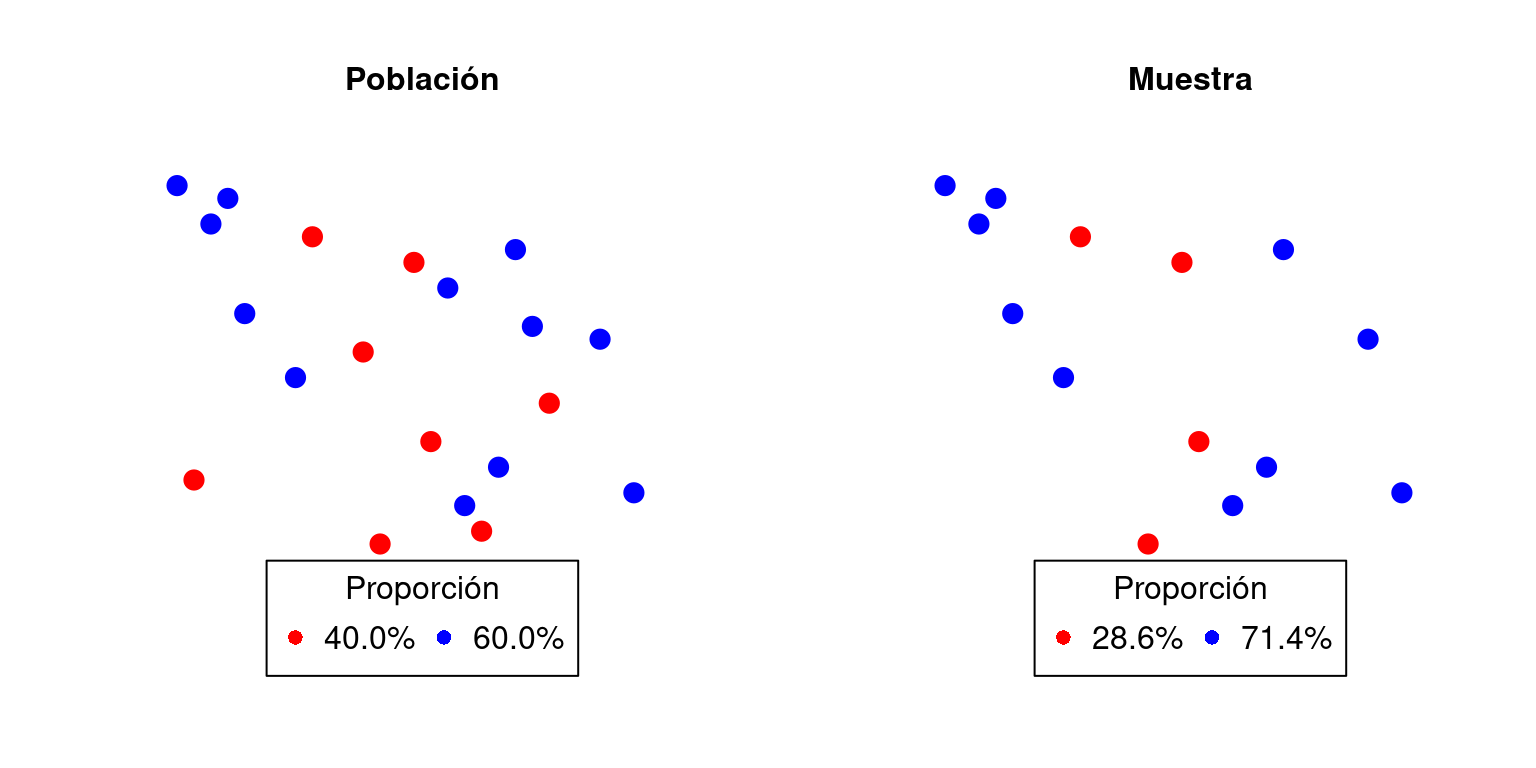
\includegraphics{estadisticas_files/figure-latex/parametro1-1} 

}

\caption{Parámetro y estadístico}\label{fig:parametro1}
\end{figure}

\subsection{Estimador y Estimación}\label{estimador-y-estimaciuxf3n}

Una extensión de los conceptos de parámetro y estadístico, son los de estimador y estimación, para los cuales, se hace la siguiente distinción:

\begin{itemize}
\item
  \textbf{Estimador}: Un estimador es un estadístico usado para aproximar (incertidumbre) el valor de un parámetro. Usualmente no cambia la técnica entre la población y la muestra, por ejemplo, si deseo aproximar la proporción de bolitas rojas en la población, se usaría la proporción de bolitas rojas en la muestra.
\item
  \textbf{Estimación}: Una estimación es el número que resulta de aplicar el estimador a una muestra particular. Esto difiera levemente de la definición anterior, ya que en términos estrictos, el estimador solo es la ``fórmula'', y la estimación es el valor resultante al aplicar la fórmula. Sin embargo, hoy en día es muy común encontrar textos en donde el estimador se considera tanto para la fórmula como para el valor obtenido.
\end{itemize}

Si consideramos un ejemplo similar al anterior (Figura \ref{fig:parametro2}), y establecemos que el \textbf{parámetro} a estudiar es la proporción de círculos rojos, es natural pensar que en la muestra (\textbf{estadístico}) el comportamiento debería ser similar. La intención de decir ``usaremos la proporción de círculos rojos en la muestra para deducir como es la proporción de círculos rojos en la población'' corresponde al \textbf{estimador} (otro tema es argumentar si esto es correcto o no), mientras que, el cálculo del estimador (cálculo de la proporción de círculos rojos en la muestra) lleva el nombre de \textbf{estimación}.

Respecto a lo anterior:

\begin{itemize}
\tightlist
\item
  ¿Cuál sería la estimación de los círculos rojos?
\item
  Si observamos la muestra de la figura \ref{fig:parametro1} y \ref{fig:parametro2}, ¿cuándo diríamos que una estimación es buena?
\end{itemize}

\begin{figure}

{\centering 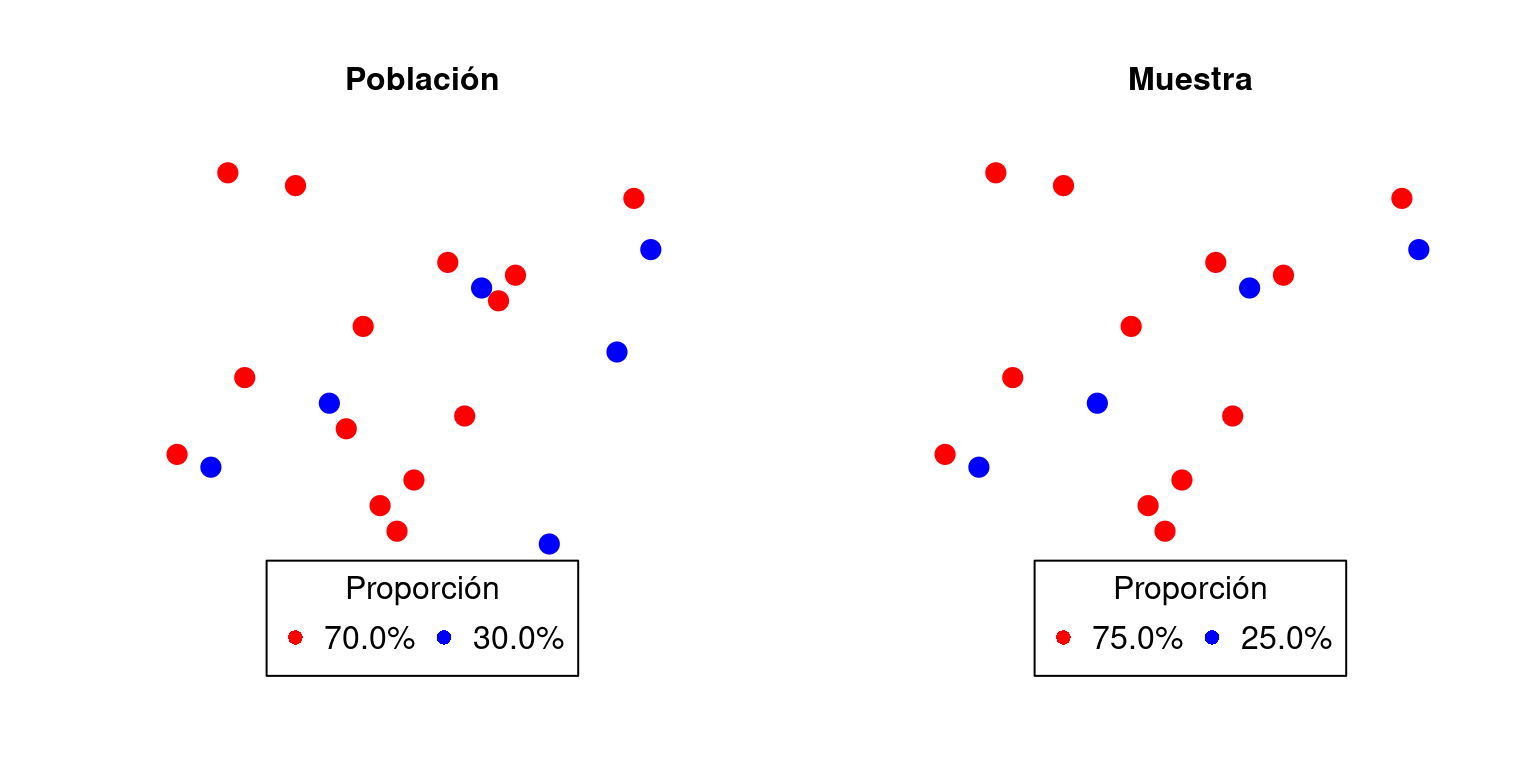
\includegraphics{estadisticas_files/figure-latex/parametro2-1} 

}

\caption{Estimador y estimación}\label{fig:parametro2}
\end{figure}

\subsection{Variabilidad muestral}\label{variabilidad-muestral}

Efectivamente, la estimación de un parámetro está determinada por la muestra con la que se trabaja. La forma en la que se elige una muestra es azarosa (que no se puede intencionar en su totalidad), por lo que es imposible saber de antemano si la estimación será buena o mala respecto al parámetro (error de estimación). En estadística, la forma en la que se elige o genera una muestra puede llegar a ser muy compleja, siendo un tema que está fuera del alcance de este curso.

El concepto detrás de esto es la \textbf{variabilidad muestral}, el cual, indica que dependiendo de la muestra que se obtenga de la población, esta se comportará distinto en relación al estadístico (igualmente para el valor del estimador: estimación). Para ilustrar esto, observemos la figura \ref{fig:figura-poblacion1}.

\textbf{¿Cuál es la proporción de círculos rojos en la población reflejada en la figura} \textbf{?}

\begin{figure}

{\centering 
\includegraphics{estadisticas_files/figure-latex/figura-poblacion1-1} 

}

\caption{Población}\label{fig:figura-poblacion1}
\end{figure}

Luego,

\textbf{¿qué podríamos inferir sobre el color predominante en la población en base a la muestra de la figura} \ref{fig:figura-muestra1}\textbf{?}

\begin{figure}

{\centering 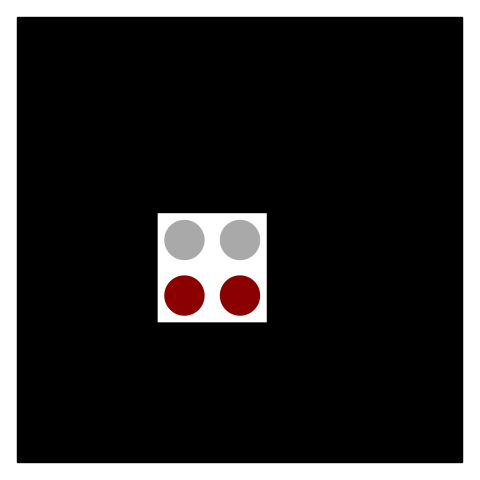
\includegraphics{estadisticas_files/figure-latex/figura-muestra1-1} 

}

\caption{Muestra 1}\label{fig:figura-muestra1}
\end{figure}

\textbf{¿Y ahora? (Figura} \ref{fig:figura-muestra2}\textbf{)}

\begin{figure}

{\centering 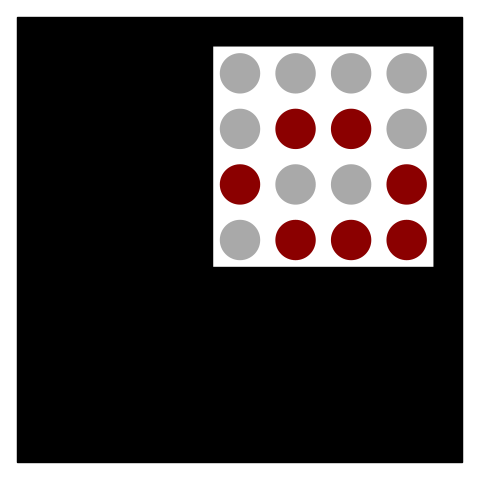
\includegraphics{estadisticas_files/figure-latex/figura-muestra2-1} 

}

\caption{Muestra 2}\label{fig:figura-muestra2}
\end{figure}

Efectivamente, diferentes muestras se comportan de manera diferente, es decir, la estimación depende de la selección de la muestra. Esto se denomina como \textbf{variabilidad muestral}.

\subsection{Representatividad y sesgo de la muestra}\label{representatividad-y-sesgo-de-la-muestra}

\begin{itemize}
\item
  \textbf{Representatividad}

  Comúnmente se escucha hablar de que una muestra debe ser representativa respecto de la población, algo muy similar a lo presentado en la sección \ref{variabilidad-muestral}. Sin embargo, este concepto no tiene sustento matemático, ya que, para poder verificar que una muestra es representativa se debe conocer a toda la población (la característica de estudio), lo cual en la práctica no ocurre. Y en caso de que se conociesen todos los datos de la población, sería absurdo calcular la estimación de un parámetro, ya que podría calcularse directamente el valor del parámetro en cuestión.
\item
  \textbf{Sesgo}

  Hay personas utilizan la siguiente frase ``\emph{la muestra está sesgada}'', lo cual es incorrecto en su totalidad en estadística. El concepto de sesgo no es únicamente propio de la estadística, sin embargo, en esta área, corresponde a una propiedad de los estimadores. Se dice que un estimador es insesgado cuando el valor esperado de este es igual al parámetro. Y al igual que el concepto anterior, no es posible verificarlo en la práctica, aunque si tiene un sustento matemático por detrás.
\end{itemize}

\section{Medidas de localización}\label{medidas-de-localizaciuxf3n}

Los resúmenes visuales de datos son herramientas excelentes para obtener impresiones y percepciones preliminares. Un análisis de datos más formal a menudo requiere el cálculo e interpretación de medidas de resumen numéricas. Es decir, de los datos se trata de extraer varios números resumidos, números que podrían servir para caracterizar el conjunto de datos. Las tres medidas de resumen más utilizadas son la media, la mediana y la moda.

\subsection{Media}\label{media}

Para un conjunto dado de números \(x_1, x_2, x_3, \ldots, x_n\), la medida más conocida y útil es la \textbf{media} o promedio aritmético. Usualmente se asume que los números \(x_i\) hace parte de una muestra, por lo que a este promedio se le connota como \textbf{media muestral} y se denota con por \(\bar{x}\).

De lo anterior, la media muestral (\(\bar{x}\)) de una conjunto de datos \(x_1, x_2, x_3, \ldots, x_n\) está dada por \citep[página 25]{Devore}

\begin{equation}
\bar{x} = \frac{x_1 + x_2 + \cdots + x_n}{n} = \frac{\displaystyle\sum_{i=1}^{n}x_i}{n}
\label{eq:promedio}
\end{equation}

En R, para obtener el promedio aritmético de los datos se hace uso de la función \textbf{mean()}. A continuación, un ejemplo.

\begin{Shaded}
\begin{Highlighting}[]
\CommentTok{\# Un conjunto de datos cualquiera}
\NormalTok{x }\OtherTok{=} \FunctionTok{c}\NormalTok{(}\DecValTok{1}\NormalTok{,}\DecValTok{2}\NormalTok{,}\DecValTok{3}\NormalTok{,}\DecValTok{6}\NormalTok{,}\DecValTok{1}\NormalTok{,}\SpecialCharTok{{-}}\DecValTok{4}\NormalTok{,}\SpecialCharTok{{-}}\DecValTok{2}\NormalTok{,}\DecValTok{6}\NormalTok{,}\DecValTok{0}\NormalTok{,}\DecValTok{10}\NormalTok{,}\SpecialCharTok{{-}}\DecValTok{20}\NormalTok{)}
\CommentTok{\# Promedio de los datos}
\FunctionTok{mean}\NormalTok{(x)}
\end{Highlighting}
\end{Shaded}

\begin{verbatim}
## [1] 0.2727273
\end{verbatim}

El promedio (\(\bar{x}\)) representa el valor central de las observaciones incluidas en una muestra. Sin embargo, esta medida puede llegar a ser inapropiada en algunas circunstancias, específicamente cuando existen valores extremos. Un ejemplo de esto, es el promedio de los ingresos (\href{https://www.ine.gob.cl/prensa/detalle-prensa/2022/07/21/el-ingreso-laboral-promedio-mensual-en-chile-fue-de-$681.039-en-2021\#:~:text=El\%20ingreso\%20laboral\%20promedio\%20mensual\%20en\%20Chile\%20fue\%20de\%20\%24681.039\%20en\%202021,-21\%2F07\%2F2022&text=El\%2050\%25\%20de\%20las\%20personas,ingreso\%20de\%20hasta\%20\%24457.690\%20mensuales.}{el caso de Chile}), ya que, es común que unos cuantos afortunados ganen cantidades astronómicas, por lo que el uso del ingreso promedio como medida de resumen puede ser engañoso (otro ejemplo, \href{https://www.google.com/finance/quote/BTC-USD?sa=X&ved=2ahUKEwi3po-_m9n8AhWUL7kGHTNFCfYQ-fUHegQIFhAe&window=MAX}{es la valorización de BitCoin al dólar estadounidense}).

A pesar de lo anterior, esta medida sigue siendo ampliamente utilizada, en gran medida porque existen muchas poblaciones para las cuales un valor extremo en la muestra sería altamente improbable (ejemplo: \href{https://www.google.com/finance/quote/EUR-CLP?window=MAX&comparison=USD-CLP}{tipo de cambio del dólar y el euro}).

\begin{exercise}
Respecto a la base \hyperref[TasaEURUSD]{Tasa Euro/Dólar}, utilice el comando \textbf{colMeans()} para obtener la media de todas las variables asociadas a la tasa de conversión (ignore la columna asociada a la variable fecha). Interprete.
\end{exercise}

\begin{exercise}
Obtenga de la media del precio por hora de la electricidad, en la base \hyperref[PreciosElectricidad]{Precios de electricidad}. Interprete.
\end{exercise}

\begin{exercise}
Considerando la base de datos \hyperref[Pacientes]{Pacientes}, determine la media del nivel de colesterol por sexo. Interprete.
\end{exercise}

\subsection{Mediana}\label{mediana}

La palabra mediana es sinónimo de ``medio'' y la mediana muestral es en realidad el valor medio una vez que se ordenan las observaciones de la más pequeña a la más grande \citep[página 26]{Devore}.

La mediana muestral se obtiene ordenando primero las observaciones de la más pequeña a la más grande. Por lo tanto,

\begin{itemize}
\tightlist
\item
  Si la cantidad de datos es impar, entonces, la mediana es igual al número en la posición \(\frac{n+1}{2}\).
\item
  Si la cantidad de datos es par, entonces, la mediana es el promedio entre los números ubicados en las posiciones \(\frac{n}{2}\) y \((\frac{n}{2}+1)\).
\end{itemize}

Para poder calcular la mediana en R, se debe hacer uso del comando \textbf{median()}, tal como se muestra a continuación.

\begin{Shaded}
\begin{Highlighting}[]
\CommentTok{\# Conjunto de datos (cantidad impar)}
\NormalTok{x }\OtherTok{=} \FunctionTok{c}\NormalTok{(}\DecValTok{1}\NormalTok{,}\DecValTok{2}\NormalTok{,}\DecValTok{3}\NormalTok{,}\DecValTok{4}\NormalTok{,}\DecValTok{5}\NormalTok{,}\DecValTok{6}\NormalTok{,}\DecValTok{7}\NormalTok{,}\SpecialCharTok{{-}}\DecValTok{3}\NormalTok{,}\SpecialCharTok{{-}}\DecValTok{1}\NormalTok{,}\SpecialCharTok{{-}}\DecValTok{2}\NormalTok{,}\FloatTok{5.4}\NormalTok{,}\FloatTok{9.3}\NormalTok{,}\DecValTok{0}\NormalTok{)}
\CommentTok{\# Mediana del conjunto de datos}
\FunctionTok{median}\NormalTok{(x)}
\end{Highlighting}
\end{Shaded}

\begin{verbatim}
## [1] 3
\end{verbatim}

\begin{Shaded}
\begin{Highlighting}[]
\CommentTok{\# Conjunto de datos (cantidad par)}
\NormalTok{x }\OtherTok{=} \FunctionTok{c}\NormalTok{(}\DecValTok{1}\NormalTok{,}\DecValTok{2}\NormalTok{,}\DecValTok{3}\NormalTok{,}\DecValTok{4}\NormalTok{,}\DecValTok{5}\NormalTok{,}\DecValTok{6}\NormalTok{,}\DecValTok{7}\NormalTok{,}\SpecialCharTok{{-}}\DecValTok{3}\NormalTok{,}\SpecialCharTok{{-}}\DecValTok{1}\NormalTok{,}\SpecialCharTok{{-}}\DecValTok{2}\NormalTok{,}\FloatTok{5.4}\NormalTok{,}\FloatTok{9.3}\NormalTok{)}
\CommentTok{\# Mediana del conjunto de datos}
\FunctionTok{median}\NormalTok{(x)}
\end{Highlighting}
\end{Shaded}

\begin{verbatim}
## [1] 3.5
\end{verbatim}

En ambos casos, se entiende que, ordenando los datos de menor a mayor (en una recta real), tanto a la derecha como izquierda de la mediana se encuentra la misma cantidad de datos.

\begin{exercise}
Obtenga la mediana de las distintas variables (cuando corresponda) de la base de datos \hyperref[Pacientes]{Pacientes}. Interprete.
\end{exercise}

\subsection{Moda}\label{moda}

La moda es la medida más intuitiva de las tres, ya que simplemente corresponde al valor que se presenta con mayor frecuencia \citep[página 85]{anderson}. Para ilustrar esto, veamos el siguiente código en R:

\begin{Shaded}
\begin{Highlighting}[]
\CommentTok{\# El siguiente vector contiene la información de la cantidad }
\CommentTok{\# de hermanos de un determinado grupo de personas}
\NormalTok{hermanos }\OtherTok{=} \FunctionTok{c}\NormalTok{(}\DecValTok{1}\NormalTok{,}\DecValTok{2}\NormalTok{,}\DecValTok{3}\NormalTok{,}\DecValTok{1}\NormalTok{,}\DecValTok{2}\NormalTok{,}\DecValTok{3}\NormalTok{,}\DecValTok{3}\NormalTok{,}\DecValTok{3}\NormalTok{,}\DecValTok{4}\NormalTok{,}\DecValTok{1}\NormalTok{,}\DecValTok{7}\NormalTok{,}\DecValTok{1}\NormalTok{,}\DecValTok{0}\NormalTok{,}\DecValTok{0}\NormalTok{,}\DecValTok{1}\NormalTok{,}\DecValTok{0}\NormalTok{,}\DecValTok{2}\NormalTok{)}
\CommentTok{\# Utilizando el comando table podemos obtener la frecuencia de }
\CommentTok{\# cada una de las distintas observaciones}
\FunctionTok{table}\NormalTok{(hermanos)}
\end{Highlighting}
\end{Shaded}

\begin{verbatim}
## hermanos
## 0 1 2 3 4 7 
## 3 5 3 4 1 1
\end{verbatim}

Como resultado se aprecia que la cantidad de hermanos que más se repita dentro del grupo de personas es de 5.

\begin{example}
\leavevmode

\begin{enumerate}
\def\labelenumi{\arabic{enumi}.}
\item
  Cree un objeto que guarde la tabla de frecuencias de la variable Open de la base de datos \hyperref[TasaEURUSD]{Tasa Euro/Dólar} (sin imprimir la tabla).

\begin{Shaded}
\begin{Highlighting}[]
\NormalTok{tabla }\OtherTok{=} \FunctionTok{table}\NormalTok{(datos}\SpecialCharTok{$}\NormalTok{Open)}
\end{Highlighting}
\end{Shaded}
\item
  Ya que es imposible buscar manualmente la frecuencia más alta, utilice el comando \textbf{which.max()} para encontrar la posición en la que se ubica esta, ingresando como argumento la tabla anteriormente guardada. Guarde este valor en un objeto.

\begin{Shaded}
\begin{Highlighting}[]
\NormalTok{(}\AttributeTok{posicion =} \FunctionTok{which.max}\NormalTok{(tabla))}
\end{Highlighting}
\end{Shaded}

\begin{verbatim}
## 1.336005 
##     3067
\end{verbatim}
\item
  Finalmente, consulte de manera directa en la tabla en valor de la frecuencia en la posición calculada en el paso anterior. Interprete.

\begin{Shaded}
\begin{Highlighting}[]
\NormalTok{tabla[posicion]}
\end{Highlighting}
\end{Shaded}

\begin{verbatim}
## 1.336005 
##        6
\end{verbatim}

  Esto quiere decir, que el valor de apertura de la tasa EUR/USD que más se repite históricamente es 1.336005 con una frecuencia de 6.

  \emph{Nota: En caso de que existan dos o más valores con las frecuencias más altas, el programa solo reporta la primera, según el orden lexicográfico de las columnas.}
\end{enumerate}

\end{example}

\begin{exercise}
Considerando la base de datos \hyperref[Pacientes]{Pacientes}, determine la moda de las variables cualitativas. Interprete.
\end{exercise}

\textbf{Nota}: En el documento se usará simplemente el nombre de la medida de localización (media, moda, mediana) para referirse a la medida de localización muestral. En casos determinados se hará la distinción entre el caso muestral y poblacional, según corresponda (ejemplo: media poblacional, media muestral).

\section{Medidas de escala}\label{medidas-de-escala}

Al momento de reportar la media solo se obtiene información parcial sobre el un conjunto de datos. Diferentes muestras o poblaciones pueden tener medidas idénticas de localización y aún diferir entre sí en otras importantes maneras. La tabla \ref{tab:variabilidad} muestra las notas obtenidas por los alumnos de 2 dos cursos con la misma media, aunque el grado de \textbf{dispersión} (variabilidad) en torno a esta es diferente para ambas muestras, es decir, en el Curso 1 las se observan notas más bajas y altas que el Curso 2.

\begin{table}[H]
\centering
\caption{\label{tab:variabilidad}Notas por curso}
\centering
\begin{tabular}[t]{ccc}
\toprule
Curso 1 & Curso 2 & Curso 3\\
\midrule
3.0 & 4.0 & 3.0\\
4.5 & 5.0 & 7.0\\
5.0 & 6.0 & --\\
5.5 & -- & --\\
7.0 & -- & --\\
\bottomrule
\end{tabular}
\end{table}

\subsection{Rango}\label{rango}

La medida más simple de variabilidad en una muestra es el \textbf{rango}, el cual es la diferencia entre los valores muestrales más grande y más pequeño \citep[página 32]{Devore}. El rango de las notas del curso 1 en la tabla \ref{tab:variabilidad} es más grande que el del curso 2, lo que refleja más variabilidad en la primer muestra que en la segunda. Un defecto del rango, no obstante, es que depende de solo las dos observaciones más extremas y hace caso omiso de las posiciones de los valores restantes. Los cursos 1 y 3 tienen rangos idénticos, aunque cuando se toman en cuenta las observaciones entre los dos extremos, existe mucho menos variabilidad o dispersión en la tercera muestra que en la primera.

\begin{example}
Obtener el rango de la tasa de apertura histórica del EUR/USD de la base de datos \hyperref[TasaEURUSD]{Tasa Euro/Dólar}.

\begin{Shaded}
\begin{Highlighting}[]
\CommentTok{\# Utilizando el comando range() se obtienen los valores mínimo y máximo}
\CommentTok{\# de la variable en cuestión}
\NormalTok{(}\AttributeTok{rango =} \FunctionTok{range}\NormalTok{(datos}\SpecialCharTok{$}\NormalTok{Open))}
\end{Highlighting}
\end{Shaded}

\begin{verbatim}
## [1] 0.959619 1.598184
\end{verbatim}

\begin{Shaded}
\begin{Highlighting}[]
\CommentTok{\# Luego calculamos la diferencia entre el valor máximo y mínimo}
\NormalTok{rango[}\DecValTok{2}\NormalTok{] }\SpecialCharTok{{-}}\NormalTok{ rango[}\DecValTok{1}\NormalTok{]}
\end{Highlighting}
\end{Shaded}

\begin{verbatim}
## [1] 0.638565
\end{verbatim}

El valor máximo siempre estará en la segunda posición y le mínimo en la segunda.
\end{example}

\begin{exercise}
Utilizando la base de datos \hyperref[Pacientes]{Paciente}, determine el rango de las variables cuantitativas. Interprete.
\end{exercise}

\begin{exercise}
Determine el rango de la fechas de medición en los precios de electricidad en la base \hyperref[PreciosElectricidad]{Precios}. Interprete.
\end{exercise}

\subsection{Varianza y desviación estándar}\label{varianza-y-desviaciuxf3n-estuxe1ndar}

Las medidas principales de variabilidad implican las \textbf{desviaciones de la media},

\begin{equation}
x_1 - \bar{x}, x_2 - \bar{x}, x_3 - \bar{x}, \ldots, x_n - \bar{x}.
\label{eq:desviaciones}
\end{equation}

Es decir, las desviaciones de la media se obtienen restando \(\bar{x}\) de cada una de las \(n\) observaciones muestrales. Una desviación será positiva si la observación es más grande que la media (a la derecha de la media sobre la recta real) y negativa si la observación es más pequeña que la media (a la izquierda de la media sobre la recta real). Si todas las desviaciones son pequeñas en magnitud, entonces todos los valores de la muestra son cercanos a la media y hay poca variabilidad. Alternativamente, si algunas de las desviaciones son grandes de magnitud, entonces algunos de los de los valores de la muestra están lejos de la media (sobre la recta real) lo que sugiere una mayor variabilidad.

Una forma de resumir las desviaciones sería sumando todas ellas. Sin embargo, es una mala idea, ya que la suma siempre es igual a cero \eqref{eq:sumadesviaciones}, ¿alguna idea del por qué?

\begin{equation}
\text{Suma de las desviaciones en una muestra} = \sum_{i=1}^{n}(x_i-\bar{x}) = 0
\label{eq:sumadesviaciones}
\end{equation}

En este sentido, para poder resumir las desviaciones de una muestra evitando el problema mencionado, se elaboran dos expresiones \citep[página 32]{Devore}:

\begin{itemize}
\tightlist
\item
  Varianza (muestral):
\end{itemize}

\begin{equation}
S^2= \frac{1}{n-1}\sum_{i=1}^{n}(x_i-\bar{x})^2
\label{eq:varianzamuestral}
\end{equation}

\begin{itemize}
\tightlist
\item
  Desviación estándar (muestral):
\end{itemize}

\begin{equation}
S = \sqrt{S^2}
\label{eq:demuestral}
\end{equation}

Las unidades correspondientes a la \textbf{varianza} suele causar confusión. Como los valores que se suman para calcular la varianza, \((x_i-\bar{x})^2\), están elevados al cuadrado, las unidades correspondientes a la varianza muestral también están elevadas al cuadrado. Las unidades al cuadrado de la varianza dificulta la compresión e interpretación intuitiva de los valores numéricos de la varianzas. Lo recomendable es entender la varianza como una medida útil para comparar la variabilidad de dos o más variables. Al comparar variables, la que tiene la varianza mayor, muestra más variabilidad. Otra interpretación del valor de la varianza suele ser innecesaria \citep[página 94]{anderson}.

La \textbf{desviación estándar} es la raíz cuadrada de la varianza, pero, ¿qué se gana con esto? Al calcular la desviación estándar, las unidades de esta son iguales a de la variable original, por lo que es más fácil de interpretar. Sin embargo, estas dos medidas tiene ciertas limitantes a la hora de comprar la variabilidad de dos variables:

\begin{enumerate}
\def\labelenumi{\arabic{enumi}.}
\tightlist
\item
  Es ideal que ambas variable tengan la misma media.
\item
  Las variables deben tener la misma unidad de medida.
\end{enumerate}

No seguir estas recomendaciones puede generar un falsa sensación en la comunicación de resultados.

\begin{example}
\protect\hypertarget{exm:EUR-USD-varianza}{}\label{exm:EUR-USD-varianza}

Compare la variabilidad entre la tasa de apertura y la tasa de cierre histórica del EUR/USD presentes en la base de datos \hyperref[TasaEURUSD]{Tasa Euro/Dólar}, para ello:

\begin{enumerate}
\def\labelenumi{\arabic{enumi}.}
\item
  Verifique la media de ambas variables la misma

\begin{Shaded}
\begin{Highlighting}[]
\FunctionTok{mean}\NormalTok{(datos}\SpecialCharTok{$}\NormalTok{Open) }\CommentTok{\# Promedio de la tasa de apertura}
\end{Highlighting}
\end{Shaded}

\begin{verbatim}
## [1] 1.244338
\end{verbatim}

\begin{Shaded}
\begin{Highlighting}[]
\FunctionTok{mean}\NormalTok{(datos}\SpecialCharTok{$}\NormalTok{Close) }\CommentTok{\# Promedio de la tasa de cierre}
\end{Highlighting}
\end{Shaded}

\begin{verbatim}
## [1] 1.244363
\end{verbatim}

  Las tasas son similares hasta el tercer decimal, se asumirá que las medias son iguales
\item
  Ya que tienen la misma unidad de medida, calcule la varianza y desviación estándar de cada una. Interprete.

  Al calcular la varianza muestral, se observa que la tasa de cierre es levemente menor variabilidad que la tasa de apertura. Similarmente, se observa que la tasa de cierre tiene menor variabilidad que la tasa de apertura.

\begin{Shaded}
\begin{Highlighting}[]
\FunctionTok{c}\NormalTok{(}\FunctionTok{var}\NormalTok{(datos}\SpecialCharTok{$}\NormalTok{Open), }\FunctionTok{var}\NormalTok{(datos}\SpecialCharTok{$}\NormalTok{Close))}
\end{Highlighting}
\end{Shaded}

\begin{verbatim}
## [1] 0.01562596 0.01562404
\end{verbatim}

\begin{Shaded}
\begin{Highlighting}[]
\FunctionTok{c}\NormalTok{(}\FunctionTok{sd}\NormalTok{(datos}\SpecialCharTok{$}\NormalTok{Open), }\FunctionTok{sd}\NormalTok{(datos}\SpecialCharTok{$}\NormalTok{Close))}
\end{Highlighting}
\end{Shaded}

\begin{verbatim}
## [1] 0.1250038 0.1249962
\end{verbatim}

  ¿Por qué es más clara la interpretación (primer decimal distinto) al utilizar la desviación estándar?
\end{enumerate}

\end{example}

\begin{exercise}
Utilice la varianza directamente para comparar la variabilidad de la variables \emph{chol}, \emph{age}, \emph{trtbps} y \emph{oldpeak} entre hombres y mujeres, en la base \hyperref[Pacientes]{Pacientes}. Interprete.
\end{exercise}

\begin{exercise}
Utilice la varianza directamente para comprar la variabilidad de los precios de la electricidad entre las primeras y últimas 1000 mediciones, en la base \hyperref[PreciosElectricidad]{Precios}. Interprete.
\end{exercise}

\subsection{Coeficiente de variación}\label{coeficiente-de-variaciuxf3n}

Para subsanar el problema de las limitaciones de la varianza y desviación estándar, se encuentra la medida llamada \textbf{coeficiente de variación} \eqref{eq:cv}.

\begin{equation}
CV = \left(\frac{S}{|\bar{x}|}\right)\cdot 100\%
\label{eq:cv}
\end{equation}

Cuando el valor del coeficiente de variación es cercano a 100\% se habla de mayor dispersión (heterogéneo), mientras que un valor cercano a 0\% indica menor dispersión (homogéneo), además, se debe considerar que el porcentaje calculado corresponde a la variabilidad respecto a la media de los datos. Sin embargo, no es recomendable usar esta medida cuando el valor de la media es cercano a cero, ya que el CV pierde su significado al tomar valores muy grandes, lo que daría una falsa sensación de dispersión de los datos \citep[página 95]{anderson}.

\begin{example}
En el ejemplo \ref{exm:EUR-USD-varianza}, se utilizó la varianza para comprar directamente la variabilidad entre la tasa de apertura y la tasa más alta histórica del EUR/USD. Sin embargo, si calculamos las medias de ambas variables se puede verificar que son distintas. Utilice el CV para comprar la variabilidad de ambas variables.

Claramente la media de la tasa más alta es mayor a la media de la tasa de apertura.

\begin{Shaded}
\begin{Highlighting}[]
\FunctionTok{c}\NormalTok{(}\FunctionTok{mean}\NormalTok{(datos}\SpecialCharTok{$}\NormalTok{Open), }\FunctionTok{mean}\NormalTok{(datos}\SpecialCharTok{$}\NormalTok{High))}
\end{Highlighting}
\end{Shaded}

\begin{verbatim}
## [1] 1.244338 1.249022
\end{verbatim}

Al verificarse una de las dos limitantes mencionadas, procedemos a calcular el CV de ambas variables.

\begin{Shaded}
\begin{Highlighting}[]
\NormalTok{CV\_Open }\OtherTok{=} \FunctionTok{sd}\NormalTok{(datos}\SpecialCharTok{$}\NormalTok{Open)}\SpecialCharTok{/}\FunctionTok{abs}\NormalTok{(}\FunctionTok{mean}\NormalTok{(datos}\SpecialCharTok{$}\NormalTok{Open))}\SpecialCharTok{*}\DecValTok{100}
\NormalTok{CV\_High }\OtherTok{=} \FunctionTok{sd}\NormalTok{(datos}\SpecialCharTok{$}\NormalTok{High)}\SpecialCharTok{/}\FunctionTok{abs}\NormalTok{(}\FunctionTok{mean}\NormalTok{(datos}\SpecialCharTok{$}\NormalTok{High))}\SpecialCharTok{*}\DecValTok{100}
\FunctionTok{c}\NormalTok{(CV\_Open, CV\_High)}
\end{Highlighting}
\end{Shaded}

\begin{verbatim}
## [1] 10.04581 10.06323
\end{verbatim}

Se puede observar que el coeficiente de variabilidad de la tasa más alta (10.06\%) es mayor a la de la tasa de apertura (10.04\%). Por lo tanto, la variabilidad (dispersión) de los datos es más homogénea para la tasa de apertura. Sin embargo, la diferencia es muy pequeña, por lo que la dispersión en relación a la media es similar entre ambas variables.
\end{example}

\begin{exercise}
Compare la variabilidad de la presión arterial en reposo y el nivel de colesterol de los pacientes registrados en la base de datos \hyperref[Pacientes]{Pacientes}. Repita el estudio diferenciado por sexo. Interprete.
\end{exercise}

\begin{exercise}
Utilizando la base de datos \hyperref[Pacientes]{Pacientes}, compare la variabilidad de la edad de los paciente, según el tipo de dolor de pecho que presentan. Interprete.
\end{exercise}

\textbf{Nota}: en el documento se usará simplemente el nombre de la medida de escala (rango, varianza, desviación estándar y CV) para referirse a la medida de escala muestral. En casos determinados se hará la distinción entre el caso muestral y poblacional, según corresponda (ejemplo: varianza poblacional, varianza muestral).

\section{Notación poblacional y muestral}\label{notaciuxf3n-poblacional-y-muestral}

\begin{table}[H]
\centering
\caption{\label{tab:notacion}Notación de parámetros y estadísticos}
\centering
\begin{tabular}[t]{lcc}
\toprule
  & Poblacional & Muestral\\
\midrule
Media & $\mu$ & $\bar{x}$\\
Varianza & $\sigma^2$ & $S^2$\\
Desviación estándar & $\sigma$ & $S$\\
\bottomrule
\end{tabular}
\end{table}

\section{Gráficos descriptivos}\label{gruxe1ficos-descriptivos}

En este apartado, se considera la representación de un conjunto de datos por medio de técnicas visuales. A continuación, se hará mención de algunas de las técnicas más útiles y pertinentes a la estadística de descriptiva. Los ejemplos presentados en esta sección hacen uso de la base de datos de la unidad (sección \ref{unidad1}).

\subsection{Histograma}\label{histograma}

Algunos datos numéricos se obtienen contando para determinar el valor de una variable (cuántas veces se repite un hecho), mientras que otro datos se obtienen tomando mediciones (peso, altura, tiempo de reacción). Usualmente, este tipo de gráfico se utiliza con datos continuos (aunque tiene una versión para datos discretos), para lo cual, se debe hacer lo siguiente \citep[página 12]{Devore}:

\begin{enumerate}
\def\labelenumi{\arabic{enumi}.}
\tightlist
\item
  Subdividir los datos en \textbf{intervalos de clase} o \textbf{clases}, de tal manera que cada observación quede contenida en exactamente una clase. Para esto, se hace uso de la regla de Sturges \citeyearpar{sturges1926choice}, la cual, consiste en calcular la expresión \(1+\log_2(n)\), aproximando hacia el entero más próximo, dónde \(n\) corresponde a la cantidad de datos (existen otra variedad de técnicas).
\item
  Determinar la frecuencia y la frecuencia relativa de cada clase, es decir, cuántas observaciones hay en cada uno de los intervalos.
\item
  Se marcan los límite de clase sobre el eje horizontal del plano cartesiano.
\item
  Se traza un rectángulo cuya altura es la frecuencia absoluta (o relativa) correspondiente a cada intervalo de clase.
\end{enumerate}

Para generar un histograma en R a partir de un conjunto de datos, se utiliza el siguiente código (se toma como ejemplo la base de datos \hyperref[TasaEURUSD]{Tasa Euro/Dólar}):

\begin{Shaded}
\begin{Highlighting}[]
\FunctionTok{library}\NormalTok{(ggplot2) }\CommentTok{\# Librería de ggplot2}
\FunctionTok{ggplot}\NormalTok{( }\CommentTok{\# Ambiente gráfico}
  \AttributeTok{data =}\NormalTok{ datos, }\CommentTok{\# Base de datos a utilizar}
       \FunctionTok{aes}\NormalTok{( }\CommentTok{\# Comandos estéticos}
         \AttributeTok{x =}\NormalTok{ Close)) }\SpecialCharTok{+} \CommentTok{\# Eje X y variable asociada }
  \FunctionTok{geom\_histogram}\NormalTok{( }\CommentTok{\# Objeto a graficar: histograma}
    \AttributeTok{bins =} \FunctionTok{round}\NormalTok{(}\DecValTok{1} \SpecialCharTok{+} \FunctionTok{log2}\NormalTok{(}\FunctionTok{dim}\NormalTok{(datos)[}\DecValTok{1}\NormalTok{])), }\CommentTok{\# Cantidad de intervalos del histograma: regla de Sturges}
    \AttributeTok{color =} \StringTok{"black"}\NormalTok{, }\CommentTok{\# Color del borde de las barras del histograma}
    \AttributeTok{fill =} \StringTok{"white"}\NormalTok{, }\CommentTok{\# Color de relleno de las barras}
    \AttributeTok{closed =} \StringTok{"left"}\NormalTok{) }\SpecialCharTok{+} \CommentTok{\# Tipo de intervalo del histograma}
  \FunctionTok{labs}\NormalTok{( }\CommentTok{\# Títulos}
    \AttributeTok{title =} \StringTok{"Histograma EUR/USD"}\NormalTok{, }\CommentTok{\# Título del gráfico}
    \AttributeTok{x =} \StringTok{"Tasa de cierre"}\NormalTok{, }\CommentTok{\# Título del eje X}
    \AttributeTok{y =} \StringTok{"Frecuencia"}\NormalTok{) }\CommentTok{\# Título del eje Y}
\end{Highlighting}
\end{Shaded}

\begin{center}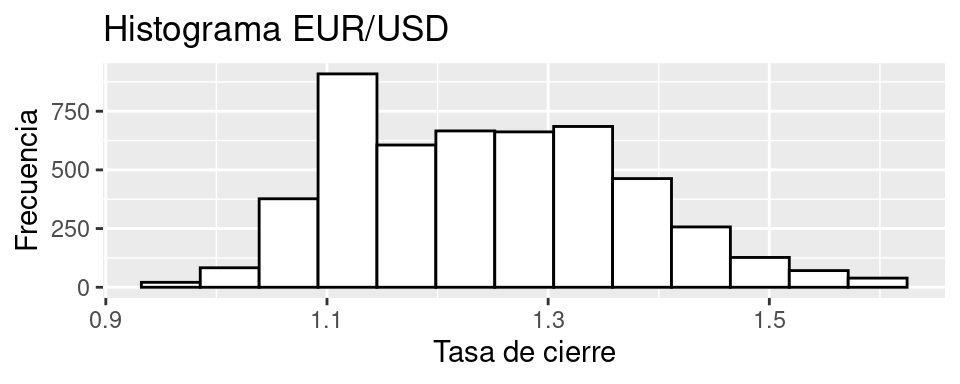
\includegraphics{estadisticas_files/figure-latex/unnamed-chunk-21-1} \end{center}

Para interpretar un histograma, basta con indicar los siguientes aspectos:

\begin{itemize}
\tightlist
\item
  Forma visual de la distribución de las barras (en general).
\item
  Mencionar si existe una concentración fuera del comportamiento general, y en dónde se encuentra.
\end{itemize}

En el caso del histograma de la tasa de cierre del EUR/USD, se observa una forma de campana centrada cerca del 1.3, además, se evidencia la presencia de una frecuencia superior al resto que se encuentra la izquierda del gráfico cerca del 1.1.

Cabe mencionar, que existen otros aspectos que son posibles mencionar, para ello consulte la bibliografía del curso.

Es útil recordar que el histograma está asociado a una tabla de frecuencia por intervalos. Para obtener la tabla asociada a un histograma se puede utilizar el siguiente código.

\begin{Shaded}
\begin{Highlighting}[]
\CommentTok{\# Datos del histograma guardados}
\NormalTok{h }\OtherTok{=} \FunctionTok{hist}\NormalTok{(datos}\SpecialCharTok{$}\NormalTok{Close, }\CommentTok{\# Datos a graficar en el histograma}
         \AttributeTok{breaks =} \DecValTok{13}\NormalTok{, }\CommentTok{\# Cantidad de intervalos: regla de Sturges}
         \AttributeTok{right =}\NormalTok{ F, }\CommentTok{\# Cerrado por la izquierda}
         \AttributeTok{plot =}\NormalTok{ F) }\CommentTok{\# No desplegar el gráfico en consola}
\FunctionTok{library}\NormalTok{(agricolae) }\CommentTok{\# Librería para generar la tabla de frecuencias}
\FunctionTok{print}\NormalTok{(}\FunctionTok{table.freq}\NormalTok{(h)) }\CommentTok{\# Imprime en consola la tabla de frecuencias}
\end{Highlighting}
\end{Shaded}

\begin{verbatim}
##    Lower Upper  Main Frequency Percentage   CF   CPF
## 1   0.95  1.00 0.975        46        0.9   46   0.9
## 2   1.00  1.05 1.025        89        1.8  135   2.7
## 3   1.05  1.10 1.075       444        8.9  579  11.7
## 4   1.10  1.15 1.125       839       16.9 1418  28.6
## 5   1.15  1.20 1.175       591       11.9 2009  40.5
## 6   1.20  1.25 1.225       634       12.8 2643  53.2
## 7   1.25  1.30 1.275       614       12.4 3257  65.6
## 8   1.30  1.35 1.325       654       13.2 3911  78.8
## 9   1.35  1.40 1.375       510       10.3 4421  89.0
## 10  1.40  1.45 1.425       257        5.2 4678  94.2
## 11  1.45  1.50 1.475       166        3.3 4844  97.5
## 12  1.50  1.55 1.525        38        0.8 4882  98.3
## 13  1.55  1.60 1.575        84        1.7 4966 100.0
\end{verbatim}

\begin{exercise}
Utilizando la base de datos de \hyperref[PreciosElectricidad]{Precios}, elabore un histograma de los precios de la electricidad. Interprete.
\end{exercise}

\subsection{Gráfico de Caja}\label{gruxe1fico-de-caja}

El gráfico de caja se utiliza para describir las siguiente características de un conjunto de datos \citep[página 35]{Devore}:

\begin{itemize}
\tightlist
\item
  El centro.
\item
  La dispersión.
\item
  El grado y naturaleza de cualquier alejamiento de la simetría.
\item
  La identificación de las observaciones ``extremas'' (atípicas) inusualmente alejadas del cuerpo principal de los datos.
\end{itemize}

Los pasos para elaborar un gráfico de caja son los siguiente \citep[página 106]{anderson}:

\begin{enumerate}
\def\labelenumi{\arabic{enumi}.}
\tightlist
\item
  Se dibuja una caja cuyos extremos se localicen en primer y tercer cuartiles. Esta caja contiene 50\% de los datos centrales.
\item
  En el punto donde se localiza la mediana se traza una linea horizontal.
\item
  Usando el rango intercuartílico (\(RIC = Q_3-Q_1\)), se localizan los límites. En un gráfico de caja los límites se encuentra a \(1.5RIC\) abajo y arriba de \(Q_1\) y \(Q_3\) respectivamente. Los datos que quedan fuera de estos límites se consideran observaciones atípicas \citep{Tukey}. La razón por la cual se considera 1.5 veces el rango intercuartílico es convencional, no obstante, hay argumento relacionados a la cantidad de datos dentro de los limites inferior y superior, los cuales indican que debe ser de 99.7\% \citep{James2013}.
\item
  Las lineas que se extienden verticalmente desde la caja se les llama \emph{bigotes}. Los bigotes van desde los extremos de la caja hasta los valores menor y mayor de los límites calculados en el paso 3.
\item
  Mediante puntos se indica la localización de las observaciones atípicas.
\end{enumerate}

Para generar un gráfico de caja en R a partir de un conjunto de datos, se utiliza el siguiente código (se toma como ejemplo la base de datos \hyperref[TasaEURUSD]{Tasa Euro/Dólar}):

\begin{Shaded}
\begin{Highlighting}[]
\NormalTok{g }\OtherTok{=} \FunctionTok{ggplot}\NormalTok{( }\CommentTok{\# Ambiente gráfico}
  \AttributeTok{data =}\NormalTok{ datos, }\CommentTok{\# Base de datos a utilizar}
  \FunctionTok{aes}\NormalTok{( }\CommentTok{\# Comandos estéticos}
    \AttributeTok{y =}\NormalTok{ Close)) }\SpecialCharTok{+} \CommentTok{\# Eje Y y variable asociada}
  \FunctionTok{geom\_boxplot}\NormalTok{( }\CommentTok{\# Objeto a graficar: gráfico de caja}
    \AttributeTok{color =} \StringTok{"black"}\NormalTok{, }\CommentTok{\# Color del borde del gráfico}
    \AttributeTok{fill =} \StringTok{"white"}\NormalTok{) }\SpecialCharTok{+} \CommentTok{\# Color de relleno del gráfico}
  \FunctionTok{labs}\NormalTok{( }\CommentTok{\# Títulos }
    \AttributeTok{title =} \StringTok{"Caja EUR/USD (opción 1)"}\NormalTok{, }\CommentTok{\# Título del gráfico}
    \AttributeTok{x =} \StringTok{""}\NormalTok{, }\CommentTok{\# Título del eje X}
    \AttributeTok{y =} \StringTok{"Tasa de cierre"}\NormalTok{) }\SpecialCharTok{+} \CommentTok{\# Título del eje Y}
  \FunctionTok{theme}\NormalTok{( }\CommentTok{\# Aspectos visuales del gráfico}
    \AttributeTok{axis.ticks.x =} \FunctionTok{element\_blank}\NormalTok{(), }\CommentTok{\# Elimina las regletas del eje X}
    \AttributeTok{axis.text.x =} \FunctionTok{element\_blank}\NormalTok{()) }\CommentTok{\# Elimina los números del eje X}
\NormalTok{info }\OtherTok{=} \FunctionTok{unlist}\NormalTok{(}\FunctionTok{ggplot\_build}\NormalTok{(g)[[}\DecValTok{1}\NormalTok{]]) }\CommentTok{\# Guardamos los valores del gráfico}
\NormalTok{values }\OtherTok{=} \FunctionTok{round}\NormalTok{(}\FunctionTok{as.numeric}\NormalTok{(info[}\DecValTok{1}\SpecialCharTok{:}\DecValTok{5}\NormalTok{]), }\DecValTok{3}\NormalTok{) }\CommentTok{\# Extraemos los valores de construcción}
\NormalTok{g1 }\OtherTok{=}\NormalTok{ g }\SpecialCharTok{+} \CommentTok{\# Creamos un nuevo gráfico a partir del anterior}
  \FunctionTok{scale\_y\_continuous}\NormalTok{( }\CommentTok{\# Modificar el eje Y}
    \AttributeTok{breaks =}\NormalTok{ values, }\CommentTok{\# Modificamos los puntos a considerar en el eje Y}
    \AttributeTok{labels =}\NormalTok{ values) }\SpecialCharTok{+} \CommentTok{\# Modificamos los valores mostrados en el eje Y}
  \FunctionTok{labs}\NormalTok{( }\CommentTok{\# Títulos}
    \AttributeTok{title =} \StringTok{"Caja EUR/USD (opción 2)"}\NormalTok{) }\CommentTok{\# Título del gráfico}
\FunctionTok{library}\NormalTok{(gridExtra) }\CommentTok{\# Librería para juntar gráficos de ggplot2}
\FunctionTok{grid.arrange}\NormalTok{(g, }\CommentTok{\# Gráfico}
\NormalTok{             g1, }\CommentTok{\# Gráfico}
             \AttributeTok{ncol =} \DecValTok{2}\NormalTok{) }\CommentTok{\# Despliegue en a dos columnas }
\end{Highlighting}
\end{Shaded}

\begin{center}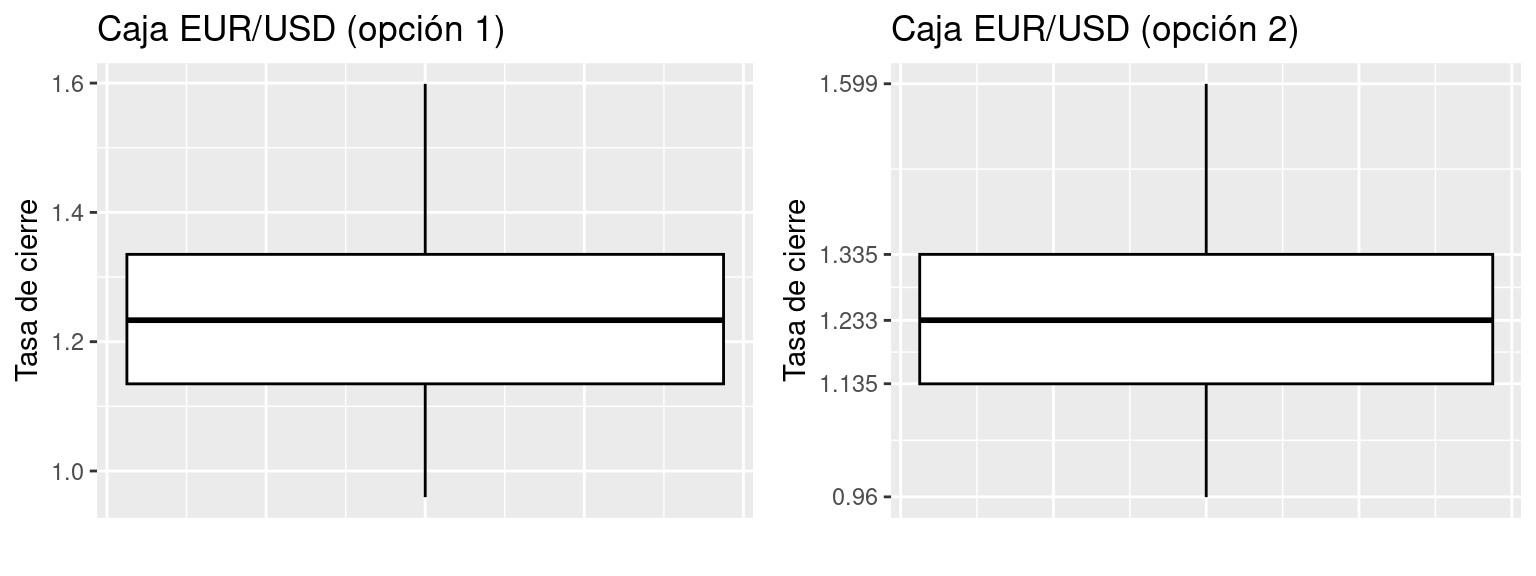
\includegraphics{estadisticas_files/figure-latex/unnamed-chunk-23-1} \end{center}

Para interpretar un gráfico de caja es recomendable utilizar la opción 2 mostrada anteriormente, ya que, se debe mencionar uno de los puntos relevantes del gráfico. En el ejemplo recién dado, se observa que, el primer, segundo y tercer cuartil están en 1.135, 1.233 y 1.335 respectivamente, mientras que el valor mínimo y máximo están en 0.96 y 1.559 respectivamente. Adicionalmente, se puede mencionar que los datos superiores en comparación a los inferiores, se encuentran más alejados de la mediana.

\begin{exercise}
Utilizando la base de datos de \hyperref[PreciosElectricidad]{Precios}, elabore un gráfico de caja de los precios de la electricidad. Interprete.
\end{exercise}

\subsection{Gráfico de Violín}\label{gruxe1fico-de-violuxedn}

El gráfico de violín proporciona una representación más completa y precisa de la distribución de los datos que las técnicas anteriores, ya que muestra tanto la forma de la distribución como su concentración \citep{hintze1998violin}. La utilidad de este gráfico recae en la comparación de la distribución de los datos entre distintos grupos y/o categorías.

El proceso de construcción del gráfico es el siguiente:

\begin{enumerate}
\def\labelenumi{\arabic{enumi}.}
\tightlist
\item
  Dibujo de la traza de densidad: la traza de densidad se dibuja sobre el eje vertical en el gráfico de violín (``forma suavizada del histograma'').
\item
  Creación de la sección central simétrica: se crea una sección central simétrica que representa la mitad de la traza de densidad.
\end{enumerate}

Adicionalmente, es común agregar un gráfico de caja junto al de violín con el fin de incorporar la visualización de las medidas de posición.

Para generar un gráfico de violín en R a partir de un conjunto de datos, se utiliza el siguiente código (se toma como ejemplo la base de datos \hyperref[TasaEURUSD]{Tasa Euro/Dólar}):

\begin{Shaded}
\begin{Highlighting}[]
\CommentTok{\# Se guarda el gráfico en una variable para posteriormente}
\CommentTok{\# integrar otros gráficos dentro de este.}
\NormalTok{g }\OtherTok{=} \FunctionTok{ggplot}\NormalTok{( }\CommentTok{\# Ambiente gráfico}
  \AttributeTok{data =}\NormalTok{ datos, }\CommentTok{\# Base de datos a utilizar}
  \FunctionTok{aes}\NormalTok{( }\CommentTok{\# Comandos estéticos}
    \AttributeTok{x =} \DecValTok{1}\NormalTok{, }\CommentTok{\# Se fija el valor horizontal del gráfico (a elección)}
    \AttributeTok{y =}\NormalTok{ Close)) }\SpecialCharTok{+} \CommentTok{\# Eje Y y variable asociada}
  \FunctionTok{geom\_violin}\NormalTok{( }\CommentTok{\# Objeto a graficar: violín}
    \AttributeTok{trim =}\NormalTok{ F, }\CommentTok{\# Modifica las terminaciones visuales superior e inferior}
    \AttributeTok{fill =} \StringTok{"white"}\NormalTok{) }\SpecialCharTok{+} \CommentTok{\# Color de relleno del gráfico}
  \FunctionTok{labs}\NormalTok{( }\CommentTok{\# Títulos}
    \AttributeTok{title =} \StringTok{"Violín EUR/USD"}\NormalTok{, }\CommentTok{\# Título del gráfico}
    \AttributeTok{x =} \StringTok{""}\NormalTok{, }\CommentTok{\# Título del eje X}
    \AttributeTok{y =} \StringTok{"Tasa de cierre"}\NormalTok{) }\SpecialCharTok{+} \CommentTok{\# Título del eje Y}
  \FunctionTok{theme}\NormalTok{( }\CommentTok{\# Aspectos visuales del gráfico}
    \AttributeTok{axis.ticks.x =} \FunctionTok{element\_blank}\NormalTok{(), }\CommentTok{\# Elimina las regletas del eje X}
    \AttributeTok{axis.text.x =} \FunctionTok{element\_blank}\NormalTok{()) }\CommentTok{\# Elimina los números del eje X}
\NormalTok{g }\CommentTok{\# Desplegamos el gráfico en el visualizador}
\end{Highlighting}
\end{Shaded}

\begin{center}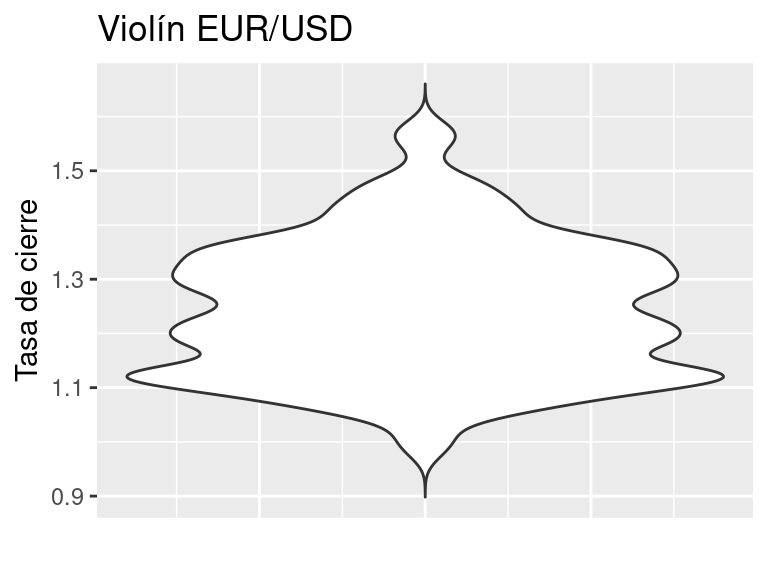
\includegraphics{estadisticas_files/figure-latex/unnamed-chunk-24-1} \end{center}

\begin{Shaded}
\begin{Highlighting}[]
\CommentTok{\# Agregamos otros elementos al gráfico guardado}
\NormalTok{g }\SpecialCharTok{+} \FunctionTok{geom\_boxplot}\NormalTok{( }\CommentTok{\# Objeto a graficar: gráfico de caja}
  \AttributeTok{width =} \FloatTok{0.1}\NormalTok{, }\CommentTok{\# Anchura proporcional del nuevo gráfico de caja}
  \AttributeTok{color =} \StringTok{"black"}\NormalTok{, }\CommentTok{\# Color de borde del gráfico}
  \AttributeTok{fill =} \StringTok{"white"}\NormalTok{) }\SpecialCharTok{+} \CommentTok{\# Color de relleno del gráfico}
  \FunctionTok{stat\_summary}\NormalTok{( }\CommentTok{\# Función para agregar información de resumen}
    \AttributeTok{fun =}\NormalTok{ mean, }\CommentTok{\# Tipo de información: promedio}
    \AttributeTok{geom =} \StringTok{"point"}\NormalTok{, }\CommentTok{\# Forma visual}
    \AttributeTok{size =} \DecValTok{1}\NormalTok{, }\CommentTok{\# Tamaño}
    \AttributeTok{color =} \StringTok{"red"}\NormalTok{, }\CommentTok{\# Color}
    \AttributeTok{orientation =} \StringTok{"x"}\NormalTok{) }\CommentTok{\# Orientación}
\end{Highlighting}
\end{Shaded}

\begin{center}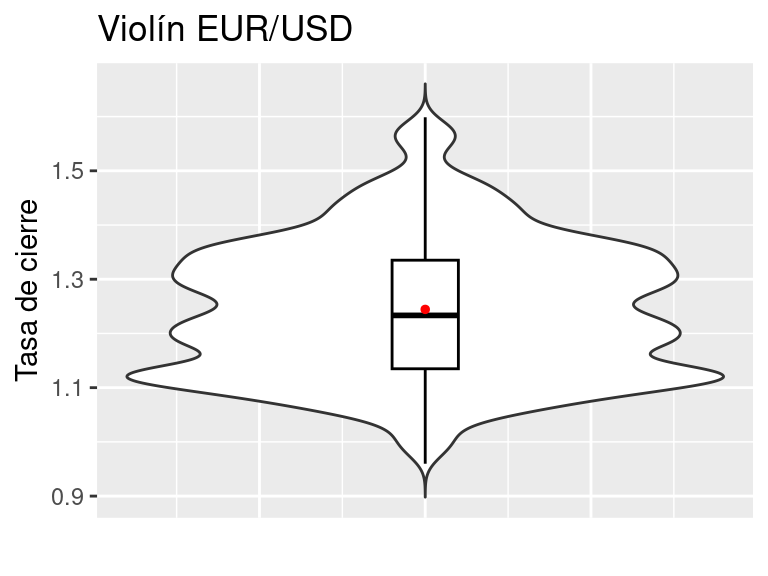
\includegraphics{estadisticas_files/figure-latex/unnamed-chunk-25-1} \end{center}

Para interpretar un gráfico de violín con caja y promedio se deben mencionar tres aspectos relevantes:

\begin{itemize}
\tightlist
\item
  Ubicación de la(s) mayor(es) concentración(es) de datos, utilizando como referencia los cuartiles.
\item
  Ubicación del promedio respecto a la mediana.
\item
  Posibles razones por las cuales se explica la ubicación anteriormente mencionada del promedio respecto a la mediana.
\end{itemize}

En el ejemplo anterior, la principal concentración se encuentra por debajo del primer cuartil, aunque destacan otras dos concentraciones que están por debajo del segundo cuartil y alrededor del tercer cuartil respectivamente. El promedio se encuentra sutilmente por encima de la mediana, esto se puede explicar debido a que los datos superiores del gráfico se encuentra más lejos de la mediana en comparación a los datos inferiores.

\begin{exercise}
Utilizando la base de datos de \hyperref[PreciosElectricidad]{Precios}, elabore un gráfico de violín con caja y promedio de los precios de la electricidad. Interprete.
\end{exercise}

\begin{example}
El siguiente código, crea una nueva columna en la base de datos que identifica el año en el que se realizó la medición de las tasas. A continuación, elabore un gráfico de violín (más gráfico de caja y promedio) de la variable \textbf{Close} en el periodo de años 2006-2010, diferenciando por año.

\begin{Shaded}
\begin{Highlighting}[]
\CommentTok{\# Extraemos el año de la variable Date, y la guardamos en un nueva columna}
\NormalTok{datos}\SpecialCharTok{$}\NormalTok{Ano }\OtherTok{=} \FunctionTok{substr}\NormalTok{(datos}\SpecialCharTok{$}\NormalTok{Date, }\DecValTok{1}\NormalTok{, }\DecValTok{4}\NormalTok{)}
\FunctionTok{ggplot}\NormalTok{( }\CommentTok{\# Ambiente gráfico}
  \AttributeTok{data =}\NormalTok{ datos[datos}\SpecialCharTok{$}\NormalTok{Ano }\SpecialCharTok{\%in\%} \DecValTok{2006}\SpecialCharTok{:}\DecValTok{2010}\NormalTok{,], }\CommentTok{\# Base de datos a utilizar}
  \FunctionTok{aes}\NormalTok{( }\CommentTok{\# Comandos estéticos}
    \AttributeTok{x =} \DecValTok{1}\NormalTok{, }\CommentTok{\# Se fija el valor horizontal del gráfico (a elección)}
    \AttributeTok{y =}\NormalTok{ Close)) }\SpecialCharTok{+} \CommentTok{\# Eje Y y variable asociada}
  \FunctionTok{geom\_violin}\NormalTok{( }\CommentTok{\# Objeto a graficar: violín}
    \AttributeTok{trim =}\NormalTok{ F, }\CommentTok{\# Modifica las terminaciones visuales superior e inferior}
    \AttributeTok{fill =} \StringTok{"white"}\NormalTok{) }\SpecialCharTok{+} \CommentTok{\# Color de relleno del gráfico}
  \FunctionTok{geom\_boxplot}\NormalTok{( }\CommentTok{\# Objeto a graficar: gráfico de caja}
    \AttributeTok{width =} \FloatTok{0.1}\NormalTok{, }\CommentTok{\# Anchura proporcional del nuevo gráfico de caja}
    \AttributeTok{color =} \StringTok{"black"}\NormalTok{, }\CommentTok{\# Color de borde del gráfico}
    \AttributeTok{fill =} \StringTok{"white"}\NormalTok{) }\SpecialCharTok{+} \CommentTok{\# Color de relleno del gráfico}
  \FunctionTok{stat\_summary}\NormalTok{( }\CommentTok{\# Función para agregar información de resumen}
    \AttributeTok{fun =}\NormalTok{ mean, }\CommentTok{\# Tipo de información: promedio}
    \AttributeTok{geom =} \StringTok{"point"}\NormalTok{, }\CommentTok{\# Forma visual}
    \AttributeTok{size =} \DecValTok{1}\NormalTok{, }\CommentTok{\# Tamaño}
    \AttributeTok{color =} \StringTok{"red"}\NormalTok{) }\SpecialCharTok{+} \CommentTok{\# Color}
  \FunctionTok{labs}\NormalTok{( }\CommentTok{\# Títulos}
    \AttributeTok{title =} \StringTok{"Violín EUR/USD"}\NormalTok{, }\CommentTok{\# Título del gráfico}
    \AttributeTok{x =} \StringTok{""}\NormalTok{, }\CommentTok{\# Título del eje X}
    \AttributeTok{y =} \StringTok{"Tasa de cierre"}\NormalTok{) }\SpecialCharTok{+} \CommentTok{\# Título del eje Y}
  \FunctionTok{theme}\NormalTok{( }\CommentTok{\# Aspectos visuales del gráfico}
    \AttributeTok{axis.ticks.x =} \FunctionTok{element\_blank}\NormalTok{(), }\CommentTok{\# Elimina las regletas del eje X}
    \AttributeTok{axis.text.x =} \FunctionTok{element\_blank}\NormalTok{()) }\SpecialCharTok{+} \CommentTok{\# Elimina los números del eje X}
  \FunctionTok{facet\_wrap}\NormalTok{( }\CommentTok{\# Segregación del gráfico}
    \FunctionTok{vars}\NormalTok{(Ano), }\CommentTok{\# Variable que se utiliza para segregar el gráfico}
    \AttributeTok{nrow =} \DecValTok{1}\NormalTok{) }\CommentTok{\# Disposición visual: una fila}
\end{Highlighting}
\end{Shaded}

\begin{center}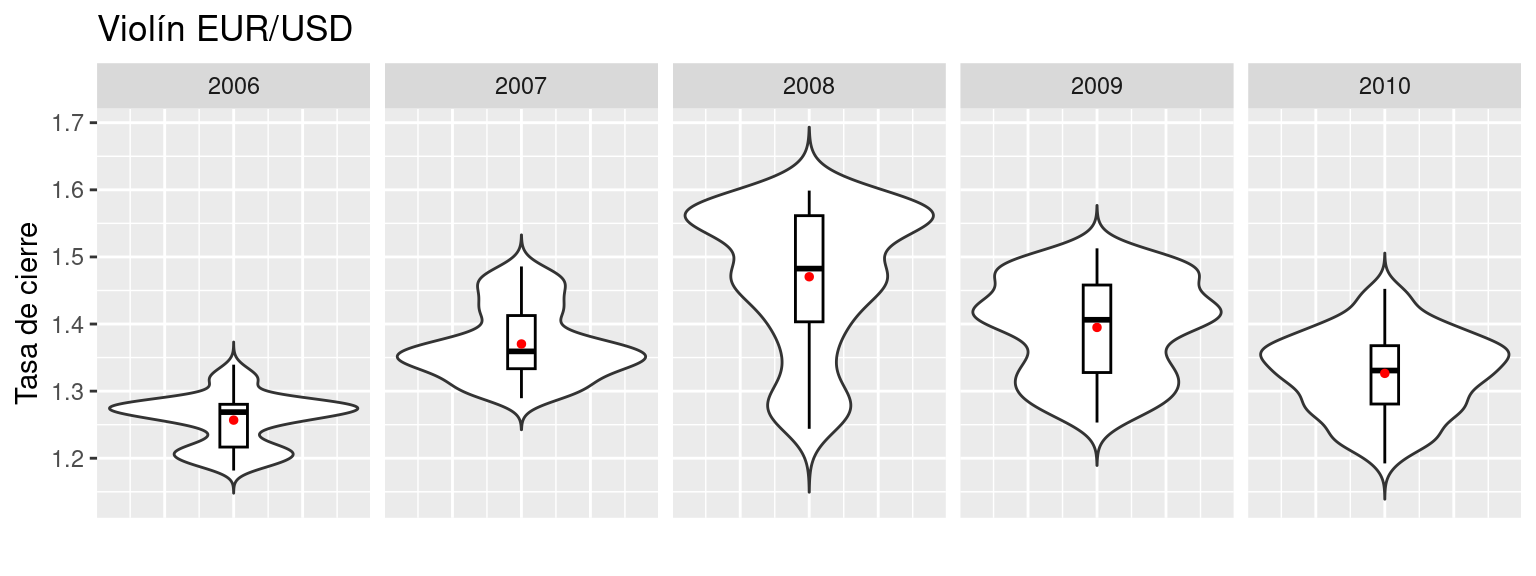
\includegraphics{estadisticas_files/figure-latex/unnamed-chunk-26-1} \end{center}

Para interpretar este tipo de gráficos, se debe realizar un interpretación uno a uno, siguiendo la recomendación antes dada. También, es posible comprar los gráficos a través de la media y coeficiente de variabilidad. Para este ejemplo, queda como trabajo del estudiante realizar esta comparación.
\end{example}

\begin{exercise}
\protect\hypertarget{exr:violin-colesterol-azucar}{}\label{exr:violin-colesterol-azucar}Utilizando la base de datos de \hyperref[Pacientes]{Paciente} Realice un gráfico de violín con caja y promedio del nivel de colesterol de los paciente, diferenciando por el nivel de azúcar en sangre en ayunas. Interprete.
\end{exercise}

\begin{exercise}
Agregue una diferenciación por sexo a lo realizado en el ejercicio \ref{exr:violin-colesterol-azucar}. Entienda que para cada nivel de azúcar en sangre se debe ver un desglose por sexo. Interprete.
\end{exercise}

\begin{exercise}
Utilizando la base de datos de \hyperref[PreciosElectricidad]{Precios}, realice un gráfico de violín con caja y promedio para el precio de la electricidad, diferenciado por año. Interprete.
\end{exercise}

\subsection{Gráfico de Barras}\label{gruxe1fico-de-barras}

Una gráfico de barras, es una gráfica para representar los datos cualitativos de una distribución de frecuencia. El procedimiento de construcción es el siguiente \citep[página 29]{anderson}.

\begin{enumerate}
\def\labelenumi{\arabic{enumi}.}
\tightlist
\item
  En uno de los ejes de la gráfica (por lo general en el horizontal), se especifican las etiquetas empleadas para las clases (categorías).
\item
  Para el otro eje de la gráfica (el vertical) se usa una escala para frecuencia, frecuencia relativa o frecuencia porcentual.
\item
  Finalmente, se emplea un ancho de barra fijo y se dibuja sobre cada etiqueta de las clases una barra que se extiende hasta la frecuencia de la clase (a diferencia del histograma, las barras deben estar separadas notoriamente).
\end{enumerate}

Para generar un gráfico de barras en R a partir de un conjunto de datos, se utiliza el siguiente código (se toma como ejemplo la base de datos \hyperref[TasaEURUSD]{Tasa Euro/Dólar}):

\begin{Shaded}
\begin{Highlighting}[]
\CommentTok{\# Nueva variable para dicotomizar la tasa de cierre del EUR/USD}
\NormalTok{datos}\SpecialCharTok{$}\NormalTok{Close2 }\OtherTok{=} \FunctionTok{ifelse}\NormalTok{(datos}\SpecialCharTok{$}\NormalTok{Close }\SpecialCharTok{\textgreater{}} \FloatTok{1.1}\NormalTok{, }\CommentTok{\# Criterio}
                      \StringTok{"Mayor a 1.1"}\NormalTok{, }\CommentTok{\# Valor asignado si se cumple el criterio}
                      \StringTok{"Menor a  1.1"}\NormalTok{) }\CommentTok{\# Valor asignado si no se cumple el criterio}
\FunctionTok{ggplot}\NormalTok{( }\CommentTok{\# Ambiente gráfico}
  \AttributeTok{data =}\NormalTok{ datos, }\CommentTok{\# Base de datos a utilizar}
  \FunctionTok{aes}\NormalTok{( }\CommentTok{\# Comandos estéticos}
    \AttributeTok{x =}\NormalTok{ Close2)) }\SpecialCharTok{+} \CommentTok{\# Eje Y y variable asociada}
  \FunctionTok{geom\_bar}\NormalTok{( }\CommentTok{\# Objeto a graficar: gráfico de barras}
    \AttributeTok{fill =} \StringTok{"white"}\NormalTok{, }\AttributeTok{color =} \StringTok{"black"}\NormalTok{) }\SpecialCharTok{+} \CommentTok{\# Color de relleno y borde}
  \FunctionTok{labs}\NormalTok{( }\CommentTok{\# Títulos}
    \AttributeTok{title =} \StringTok{"Barras EUR/USD"}\NormalTok{, }\CommentTok{\# Título del gráfico}
    \AttributeTok{x =} \StringTok{"Tasa de cierre"}\NormalTok{, }\CommentTok{\# Título del eje X}
    \AttributeTok{y =} \StringTok{"Frecuencia"}\NormalTok{) }\CommentTok{\# Título del eje Y}
\end{Highlighting}
\end{Shaded}

\begin{center}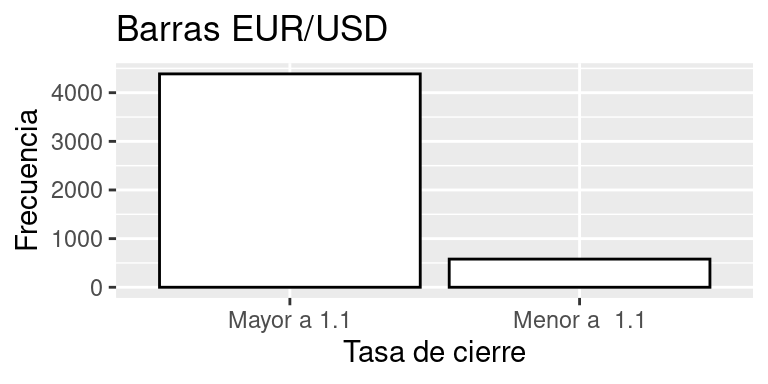
\includegraphics{estadisticas_files/figure-latex/unnamed-chunk-27-1} \end{center}

La interpretación de este tipo de gráfico (gráfico de barras no apiladas) es bastante intuitiva, ya que consiste en mencionar cuál categoría tiene un mayor frecuencia. En caso de graficar una variable con más de 2 categorías, se debe mencionar a que altura del eje vertical se encuentra la altura de cada una de las barras. Para obtener mayor detalles respecto a las frecuencias por categoría, suele apoyarse con un tabla de frecuencias absolutas o relativas porcentuales.

En el ejemplo, la frecuencia de la cantidad de tasas de cierre que se encuentran por sobre 1.1 es mayor a las que se encuentran por debajo, con una frecuencia sobre 4000 y menor a 1000 respectivamente.

\begin{exercise}
Utilizando la base de datos \hyperref[Pacientes]{Pacientes}, elabore un gráfico de barras de la variable \emph{fbs}. Interprete, apoyado de una tabla de frecuencias absolutas.
\end{exercise}

\begin{exercise}
Utilizando la base de datos \hyperref[Pacientes]{Pacientes}, elabore un gráfico de barras (no apiladas) de la variable \emph{cp}, diferenciado por sexo. Interprete, apoyado de una tabla de frecuencias relativas porcentuales. Haga el contraste visual con el gráfico de barras apiladas.
\end{exercise}

\subsection{Gráfico de Dispersión}\label{gruxe1fico-de-dispersiuxf3n}

El gráfico de dispersión es útil para estudiar la relación entre dos variables continuas. Muestra cómo varía un variable en función de la otra y puede ayudar a identificar patrones y tendencias \citep{rowlingson2016data}.

Los pasos para elaborar un gráfico de caja son los siguiente \citep{healy2019data}:

\begin{enumerate}
\def\labelenumi{\arabic{enumi}.}
\tightlist
\item
  Elegir dos variables continuas de la base de datos a trabajar. Cada fila corresponde a una observación, por lo cual, hay una correspondencia entre los valores de una misma fila.
\item
  Elegir la variable estará en el eje X y Y.
\item
  Representar cada par ordenado con un punto.
\end{enumerate}

Para generar un gráfico de dispersión en R a partir de un conjunto de datos, se utiliza el siguiente código (se toma como ejemplo la base de datos \hyperref[TasaEURUSD]{Tasa Euro/Dólar}):

\begin{Shaded}
\begin{Highlighting}[]
\FunctionTok{ggplot}\NormalTok{( }\CommentTok{\# Ambiente gráfico}
  \AttributeTok{data =}\NormalTok{ datos, }\CommentTok{\# Base de datos a utilizar}
  \FunctionTok{aes}\NormalTok{( }\CommentTok{\# Comando estéticos}
    \AttributeTok{x =}\NormalTok{ Open, }\CommentTok{\# Eje X y variable asociada}
    \AttributeTok{y =}\NormalTok{ Close)) }\SpecialCharTok{+} \CommentTok{\# Eje Y y variable asociada}
  \FunctionTok{geom\_point}\NormalTok{( }\CommentTok{\# Objeto a graficar: Gráfico de dispersión}
    \AttributeTok{color =} \StringTok{"black"}\NormalTok{, }\CommentTok{\# Color}
    \AttributeTok{alpha =} \FloatTok{0.3}\NormalTok{) }\SpecialCharTok{+} \CommentTok{\# Opacidad}
  \FunctionTok{labs}\NormalTok{( }\CommentTok{\# Títulos}
    \AttributeTok{title =} \StringTok{"Tasa de apertura y cierre del EUR/USD"}\NormalTok{, }\CommentTok{\# Título del gráfico}
    \AttributeTok{x =} \StringTok{"Tasa de apertura"}\NormalTok{, }\CommentTok{\# Título del eje X}
    \AttributeTok{y =} \StringTok{"Tasa de cierre"}\NormalTok{) }\CommentTok{\# Título del eje Y}
\end{Highlighting}
\end{Shaded}

\begin{center}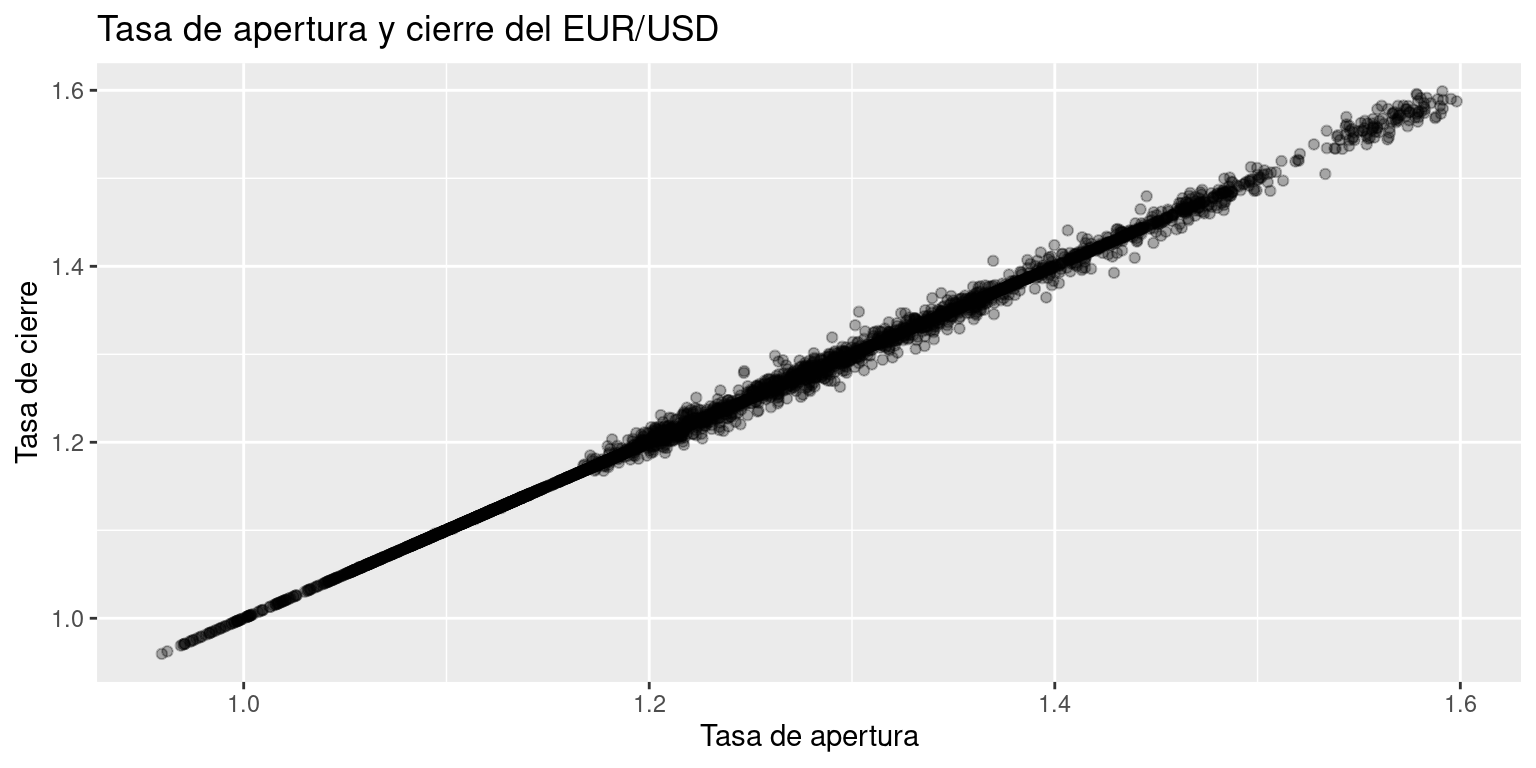
\includegraphics{estadisticas_files/figure-latex/unnamed-chunk-28-1} \end{center}

Tal como se menciona al inicio, la interpretación de este tipo de gráficos radica en describir la tendencia de los puntos. En el ejemplo anterior, el gráfico muestra una tendencia al alza, es decir, que cuando la tasa de apertura del EUR/USD aumenta, entonces, la tasa de cierre tiende a aumentar.

\begin{exercise}
Utilizando la base de datos \hyperref[Pacientes]{Pacientes}, realice un gráfico de dispersión entre la variable \emph{age} (eje X) y la variable \emph{thalachh} (eje Y). Interprete.
\end{exercise}

\begin{example}

En los siguiente gráficos se toma como ejemplo la base de datos \hyperref[TasaEURUSD]{Tasa Euro/Dólar}.

\begin{enumerate}
\def\labelenumi{\arabic{enumi}.}
\item
  Es posible utilizar el gráfico de dispersión con variables que en su naturaleza son discretas. En este sentido, elabore un gráfico de dispersión entre el año de medición y el valor promedio de tasa de apertura del EUR/USD (guarde el gráfico en una variable).

\begin{Shaded}
\begin{Highlighting}[]
\NormalTok{g }\OtherTok{=} \FunctionTok{ggplot}\NormalTok{( }\CommentTok{\# Ambiente gráfico}
  \AttributeTok{data =}\NormalTok{ datos, }\CommentTok{\# Base de datos a utilizar}
  \FunctionTok{aes}\NormalTok{( }\CommentTok{\# Comando estéticos}
\AttributeTok{x =}\NormalTok{ Ano, }\CommentTok{\# Eje X y variable asociada}
\AttributeTok{y =}\NormalTok{ Open, }\CommentTok{\# Eje Y y variable asociada}
\AttributeTok{group =} \DecValTok{1}\NormalTok{)) }\SpecialCharTok{+} \CommentTok{\# Comando únicamente necesario para la pregunta 2}
  \FunctionTok{geom\_point}\NormalTok{( }\CommentTok{\# Objeto a graficar}
\AttributeTok{stat =} \StringTok{"summary"}\NormalTok{, }\CommentTok{\# Tipo de información a graficar: resumen}
\AttributeTok{fun =} \StringTok{"mean"}\NormalTok{) }\SpecialCharTok{+} \CommentTok{\# Tipo de resumen: promedio de la variable Y}
  \FunctionTok{labs}\NormalTok{( }\CommentTok{\# Títulos}
\AttributeTok{title =} \StringTok{"Tasa de apertura promedio del EUR/USD por año"}\NormalTok{, }\CommentTok{\# Título del gráfico}
\AttributeTok{x =} \StringTok{"Año"}\NormalTok{, }\CommentTok{\# Título del eje X}
\AttributeTok{y =} \StringTok{"Tasa de apertura"}\NormalTok{) }\CommentTok{\# Título del eje Y}
\NormalTok{g }\CommentTok{\# Desplegamos el gráfico guardado}
\end{Highlighting}
\end{Shaded}

  \begin{center}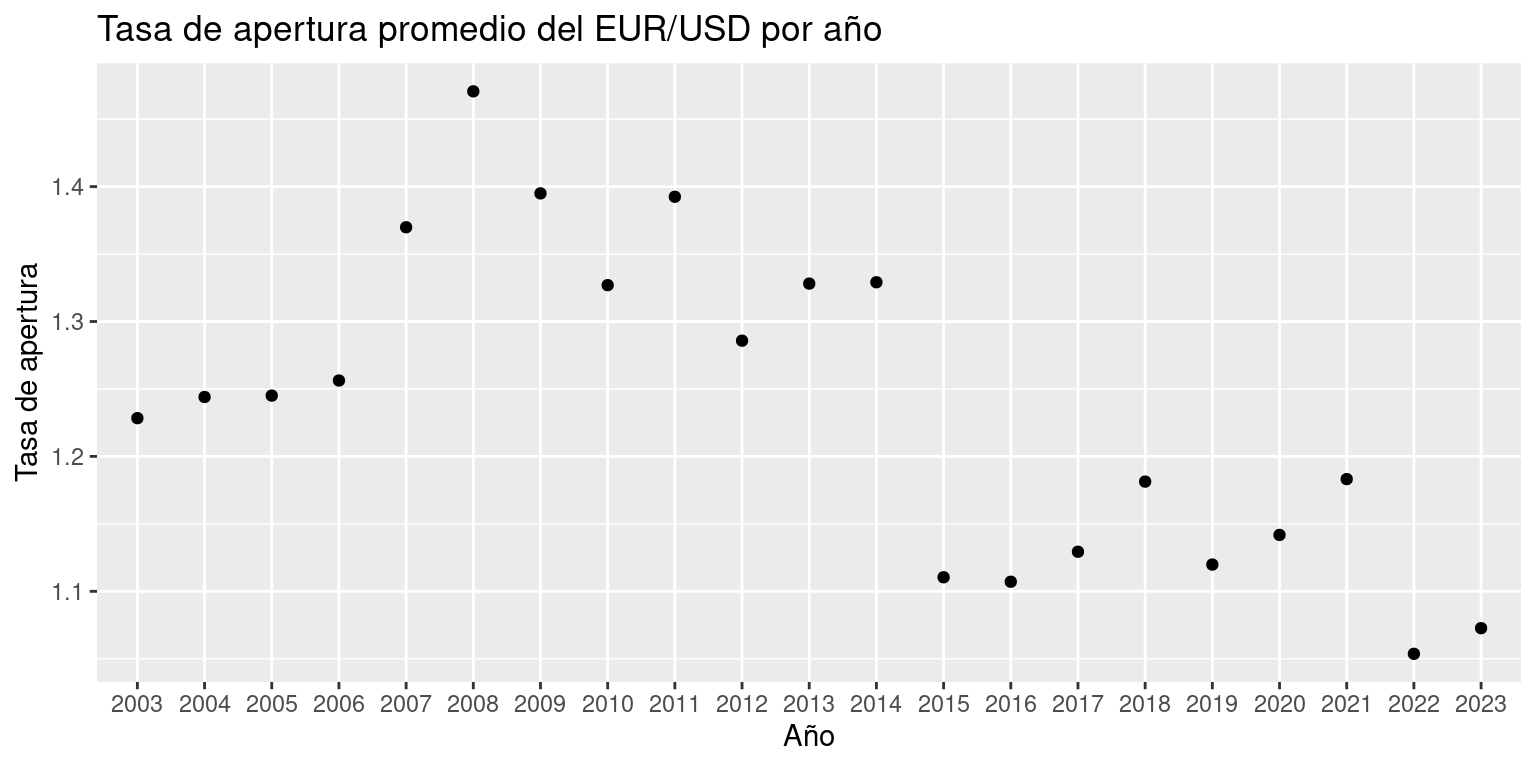
\includegraphics{estadisticas_files/figure-latex/unnamed-chunk-29-1} \end{center}
\item
  Añadir al gráfico un formato de líneas entre los puntos. Interprete.

\begin{Shaded}
\begin{Highlighting}[]
\NormalTok{g }\OtherTok{=}\NormalTok{ g }\SpecialCharTok{+} \CommentTok{\# Añadimos otro gráfico}
  \FunctionTok{geom\_line}\NormalTok{( }\CommentTok{\# Objeto a graficar: lineas}
\AttributeTok{stat =} \StringTok{"summary"}\NormalTok{, }\CommentTok{\# Tipo de información a graficar: resumen}
\AttributeTok{fun =} \StringTok{"mean"}\NormalTok{) }\CommentTok{\# Tipo de resumen: promedio de la variable Y}
\NormalTok{g }\CommentTok{\# Desplegamos el gráfico guardado}
\end{Highlighting}
\end{Shaded}

  \begin{center}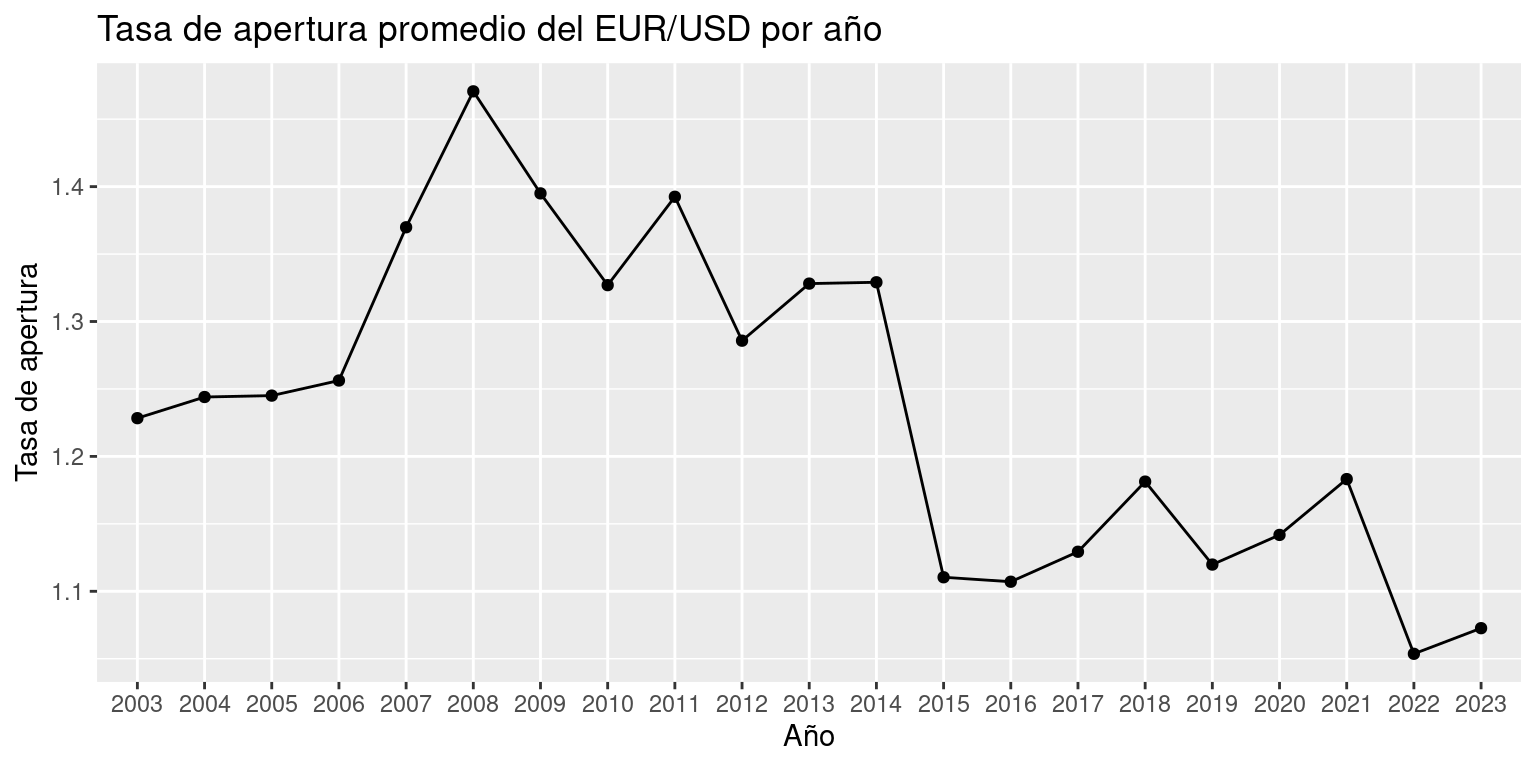
\includegraphics{estadisticas_files/figure-latex/unnamed-chunk-30-1} \end{center}

  Hasta el 2008 la tasa promedio de apertura estuvo en alza, posteriormente, la tasa decayó a un valor inferior a 1.1.
\item
  Grafique el valor de la tasa de apertura del EUR/USD desde el 2020 hasta el 2022 separadamente. Interprete.

\begin{Shaded}
\begin{Highlighting}[]
\NormalTok{datos}\SpecialCharTok{$}\NormalTok{Date }\OtherTok{=} \FunctionTok{as.Date}\NormalTok{(datos}\SpecialCharTok{$}\NormalTok{Date) }\CommentTok{\# Fechas en formato fecha de R}
\NormalTok{g }\OtherTok{=} \FunctionTok{ggplot}\NormalTok{( }\CommentTok{\# Ambiente gráfico}
  \AttributeTok{data =}\NormalTok{ datos[datos}\SpecialCharTok{$}\NormalTok{Ano }\SpecialCharTok{\%in\%} \DecValTok{2020}\SpecialCharTok{:}\DecValTok{2022}\NormalTok{,], }\CommentTok{\# Datos de los años 2020 al 2022}
  \FunctionTok{aes}\NormalTok{( }\CommentTok{\# Comando estéticos}
\AttributeTok{x =}\NormalTok{ Date, }\CommentTok{\# Comandos estéticos: Eje X y variable asociada}
\AttributeTok{y =}\NormalTok{ Open)) }\SpecialCharTok{+} \CommentTok{\# Eje Y y variable asociada}
  \FunctionTok{geom\_point}\NormalTok{( }\CommentTok{\# Objeto a graficar}
\AttributeTok{alpha =} \FloatTok{0.5}\NormalTok{, }\CommentTok{\# Opacidad}
\AttributeTok{size =} \FloatTok{0.6}\NormalTok{) }\SpecialCharTok{+} \CommentTok{\# Tamaño}
  \FunctionTok{theme}\NormalTok{( }\CommentTok{\# Aspectos visuales del gráfico}
\AttributeTok{axis.text.x =} \FunctionTok{element\_blank}\NormalTok{()) }\SpecialCharTok{+} \CommentTok{\# Eliminamos el texto del eje X}
  \FunctionTok{facet\_wrap}\NormalTok{( }\CommentTok{\# Segregación del gráfico}
\FunctionTok{vars}\NormalTok{(Ano), }\CommentTok{\# Variable que se utiliza para segregar el gráfico}
\AttributeTok{nrow =} \DecValTok{1}\NormalTok{, }\CommentTok{\# Disposición visual: una fila}
\AttributeTok{scales =} \StringTok{"free\_x"}\NormalTok{) }\SpecialCharTok{+} \CommentTok{\# La escala del eje X es independiente para gráfico}
  \FunctionTok{labs}\NormalTok{( }\CommentTok{\# Títulos}
\AttributeTok{title =} \StringTok{"Tasa de apertura del EUR/USD desde el 2020 hasta el 2022"}\NormalTok{, }\CommentTok{\# Título del gráfico}
\AttributeTok{x =} \StringTok{"Fecha"}\NormalTok{, }\CommentTok{\# Título del eje X}
\AttributeTok{y =} \StringTok{"Tasa de apertura"}\NormalTok{) }\CommentTok{\# Título del eje Y}
\NormalTok{g }\CommentTok{\# Desplegamos el gráfico guardado}
\end{Highlighting}
\end{Shaded}

  \begin{center}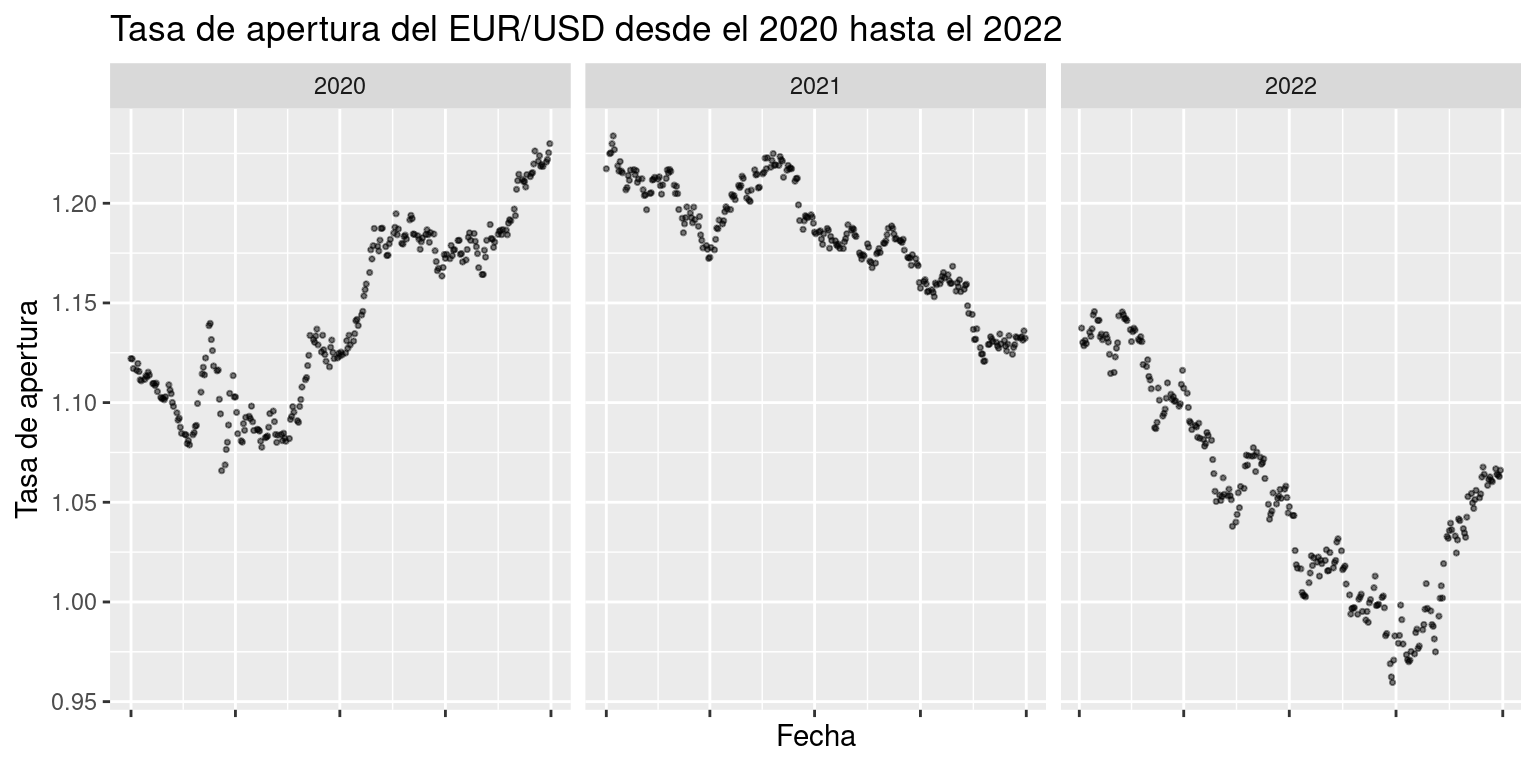
\includegraphics{estadisticas_files/figure-latex/unnamed-chunk-31-1} \end{center}

  Durante los 3 años consecutivos, se observa que únicamente en el 2020 la tendencia de la tasa de apertura es al alza, mientra que para los otros dos años hubo un decaimiento en el valor de esta.
\item
  Grafique el valor de la tasa de apertura del EUR/USD diferenciando por año. Interprete.

\begin{Shaded}
\begin{Highlighting}[]
\NormalTok{g }\OtherTok{=} \FunctionTok{ggplot}\NormalTok{( }\CommentTok{\# Ambiente gráfico}
  \AttributeTok{data =}\NormalTok{ datos, }\CommentTok{\# Base de datos a utilizar}
  \FunctionTok{aes}\NormalTok{( }\CommentTok{\# Comando estéticos}
\AttributeTok{x =}\NormalTok{ Date, }\CommentTok{\# Comandos estéticos: Eje X y variable asociada}
\AttributeTok{y =}\NormalTok{ Open, }\CommentTok{\# Eje Y y variable asociada}
\AttributeTok{color =}\NormalTok{ Ano)) }\SpecialCharTok{+} \CommentTok{\# Color según el año}
  \FunctionTok{geom\_point}\NormalTok{( }\CommentTok{\# Objeto a graficar}
\AttributeTok{alpha =} \FloatTok{0.5}\NormalTok{, }\CommentTok{\# Opacidad}
\AttributeTok{size =} \FloatTok{0.7}\NormalTok{) }\SpecialCharTok{+} \CommentTok{\# Tamaño}
  \FunctionTok{labs}\NormalTok{( }\CommentTok{\# Títulos}
\AttributeTok{color =} \StringTok{"Año"}\NormalTok{, }\CommentTok{\# Título de la leyenda}
\AttributeTok{title =} \StringTok{"Tasa de apertura del EUR/USD"}\NormalTok{, }\CommentTok{\# Título del gráfico}
\AttributeTok{x =} \StringTok{"Fecha"}\NormalTok{, }\CommentTok{\# Título del eje X}
\AttributeTok{y =} \StringTok{"Tasa de apertura"}\NormalTok{) }\SpecialCharTok{+} \CommentTok{\# Título del eje Y}
  \FunctionTok{guides}\NormalTok{( }\CommentTok{\# Edición de escalas}
\AttributeTok{color =} \FunctionTok{guide\_legend}\NormalTok{( }\CommentTok{\# Escala de color de la leyenda}
  \AttributeTok{override.aes =} \FunctionTok{list}\NormalTok{( }\CommentTok{\# Comando estéticos asociados}
    \AttributeTok{alpha =} \DecValTok{1}\NormalTok{, }\CommentTok{\# Opacidad de los puntos}
    \AttributeTok{size =} \DecValTok{3}\NormalTok{))) }\CommentTok{\# Tamaño de los puntos}
\NormalTok{g }\CommentTok{\# Desplegamos el gráfico guardado}
\end{Highlighting}
\end{Shaded}

  \begin{center}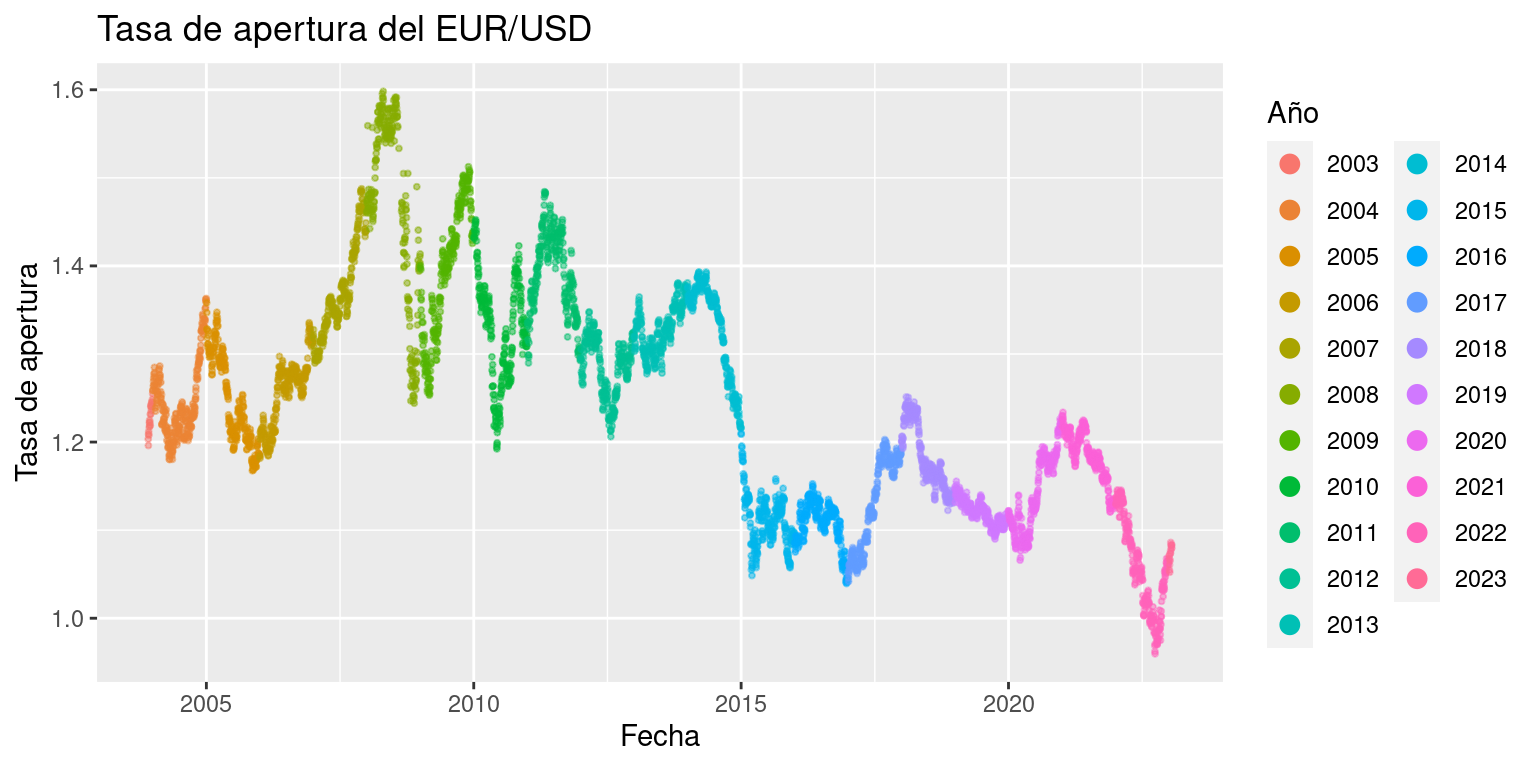
\includegraphics{estadisticas_files/figure-latex/unnamed-chunk-32-1} \end{center}

  Al observar la evolución histórica de la tasa de apertura diferenciada por año, se aprecia que el periodo 2008 - 2010 es aquel con predominancia de valores más altos. Por otro lado, desde el 2016, se registraron pro primera vez valores menores a 1.1. En años posteriores, no ha observado que la tasa supere los 1.3 puntos.
\end{enumerate}

\end{example}

\begin{exercise}

Utilizando la base de datos de la \hyperref[TasaEURUSD]{Tasa Euro/Dólar}:

\begin{enumerate}
\def\labelenumi{\arabic{enumi}.}
\tightlist
\item
  Elabore un gráfico de dispersión entre el año de medición y el valor promedio de tasa de cierre del EUR/USD (guarde el gráfico en una variable).
\item
  Añadir al gráfico un formato de líneas entre los puntos. Interprete.
\item
  Grafique el valor de la tasa de cierre del EUR/USD desde el 2010 hasta el 2013 separadamente. Interprete.
\item
  Grafique el valor de la tasa de cierre del EUR/USD diferenciando por año. Interprete.
\end{enumerate}

\end{exercise}

\begin{exercise}
Utilizando la base de datos de \hyperref[PreciosElectricidad]{Precios de electricidad}, elabore un gráfico de dispersión del precio de la electricidad a través del tiempo (considere año, mes y día). Interprete.
\end{exercise}

\begin{exercise}

Utilizando la base de datos de \hyperref[Pacientes]{Pacientes}:

\begin{enumerate}
\def\labelenumi{\arabic{enumi}.}
\tightlist
\item
  Elabore un histograma del nivel de colesterol de los pacientes. Interprete.
\item
  Elabore un gráfico de caja del nivel de colesterol de los pacientes, diferenciando por sexo. Interprete y compare.
\item
  Elabore un gráfico de violín (más caja y promedio) del nivel de colesterol de los pacientes, diferenciado por tipo de dolor en el pecho. Interprete y compare.
\item
  Elabore un gráfico de dispersión entre la edad (eje X) y el nivel de colesterol (eje Y) de los pacientes, coloreando por sexo. Interprete.
\end{enumerate}

\end{exercise}

\chapter{Probabilidad y variables aleatorias}\label{probabilidad-y-variables-aleatorias}

\section{Elementos de probabilidad}\label{elementos-de-probabilidad}

Los elementos de probabilidad son los conceptos fundamentales que se utilizan en la teoría de la probabilidad para describir y analizar eventos aleatorios. Algunos de ellos son: espacio muestral, eventos, función de probabilidad, variable aleatoria, distribución de probabilidad, entre otros.

Estos elementos son esenciales para el estudio de la probabilidad y su aplicación en la estadística y en muchas áreas de la ciencia, incluyendo la economía, la biología, la física, entre otras.

\subsection{Experimento y Espacio muestral}\label{experimento-y-espacio-muestral}

En el contexto de la probabilidad, un \textbf{experimento} es definido como un proceso que genera resultados definidos. Y en cada una de las repeticiones del experimento, habrá uno y solo uno de los posibles resultados experimentales \citep[página 143]{anderson}.

\begin{example}
\leavevmode

\begin{table}[H]
\centering
\caption{\label{tab:experimentos}Experimentos y resultados}
\centering
\begin{tabular}[t]{ll}
\toprule
Experimento & Resultado experimental\\
\midrule
Lanzar una moneda & Cara, cruz\\
Tomar una pieza para inspeccionarla & Con defecto, sin defecto\\
Realizar una llamada de ventas & Hay compra, no hay compra\\
Lanzar un dado & 1, 2, 3, 4, 5, 6\\
Jugar un partido de fútbol & Ganar, perder, empatar\\
\bottomrule
\end{tabular}
\end{table}

\end{example}

Al especificar todos los resultados experimentales posibles, se está definiendo el \textbf{espacio muestral} de un experimento. En otras palabras, el espacio muestral de un experimentos es el conjunto de todos los resultados experimentales. Se usa la letra omega mayúscula (\(\Omega\)) para referirnos a este conjunto. Un elemento genérico de \(\Omega\) se denota como \(\omega\).

\begin{example}
Conduciendo hacia su trabajo, una persona debe pasar por tres semáforos. En cada cruce la persona puede detenerse (D) o continuar (C), de acuerdo con el color de la luz. ¿Cuál es el espacio muestral del experimento?

\[\Omega = \lbrace CCC, DDD, CCD, CDD, CDC, DCD, DDC, DCC \rbrace\]
\end{example}

\begin{exercise}
Un fabricante de ropa deportiva produce pantalones deportivos en dos colores (azul y gris) y en cuatro tamaños diferentes (pequeño, mediano, grande y extra grande). ¿Cuál es el espacio muestral del experimento de elegir al azar un pantalón deportivo de la línea de producción de la empresa?
\end{exercise}

\begin{exercise}
Un restaurante ofrece tres opciones de menú para el almuerzo: menú A, menú B y menú C. Además, cada menú se puede pedir con carne o con pescado. ¿Cuál es el espacio muestral del experimento de elegir al azar un menú para el almuerzo en este restaurante?
\end{exercise}

\begin{exercise}
Una compañía de seguros de autos ofrece pólizas de seguro con dos niveles de cobertura (básico y completo) y dos tipos de franquicia (alta y baja). ¿Cuál es el espacio muestral del experimento de elegir al azar una póliza de seguro de auto de la compañía?
\end{exercise}

\subsection{Eventos aleatorios}\label{eventos-aleatorios}

En principio, un \textbf{evento aleatorio} (o simplemente evento) es algún subconjunto del espacio muestral \(\Omega\). Los eventos se anotan con una letra mayúscula a elección \citep[página 153]{anderson}.

A modo de ejemplo, consideren el experimento de lanzar un dado de 6 caras.

\(\Omega = \lbrace 1,2,3,4,5,6 \rbrace\)

Luego, el evento correspondiente a obtener un número par está dado por:

A: obtener un número par \(\rightarrow A = \lbrace 2,4,6 \rbrace\)

\begin{exercise}
Experimento aleatorio: Lanzamiento de un dado. Evento aleatorio: Obtener un número impar. ¿Cuál es el conjunto correspondiente al evento aleatorio?
\end{exercise}

\begin{exercise}
Experimento aleatorio: Elegir una carta al azar de una baraja inglesa de 52 cartas. Evento aleatorio: Obtener una carta roja. ¿Cuál es el conjunto correspondiente al evento aleatorio?
\end{exercise}

\begin{exercise}
Experimento aleatorio: Lanzar dos monedas. Evento aleatorio: Obtener dos caras. ¿Cuál es el conjunto correspondiente al evento aleatorio?
\end{exercise}

\begin{exercise}
Experimento aleatorio: Elegir un estudiante al azar de una clase de 30 estudiantes. Evento aleatorio: Elegir a un estudiante que tenga una altura superior a 1,75 metros. ¿Cuál es el conjunto correspondiente al evento aleatorio?
\end{exercise}

\begin{exercise}
Experimento aleatorio: Lanzar un dardo a una diana circular (el centro y 6 sectores circulares). Evento aleatorio: Obtener un lanzamiento dentro del círculo exterior de la diana. ¿Cuál es el conjunto correspondiente al evento aleatorio?
\end{exercise}

\subsection{Probabilidad de un evento}\label{probabilidad-evento}

El concepto de probabilidad está asociado a la ocurrencia de un evento Sin embargo, el número que determina que tan factible es que dicho evento ocurra puede ser difícil de calcular. En este aspecto, como introducción, se hará uso de la definición clásica de probabilidad:

\emph{Probabilidad de que ocurra un evento} \(= \displaystyle\frac{\text{Casos favorables}}{\text{Casos totales}}\)

Por ejemplo, la probabilidad de obtener un número par al lanzar un dado una vez es:

A: obtener un número par. \(\rightarrow A = \lbrace 2,4,6 \rbrace\)

\[P(A) = \frac{\text{Casos favorables}}{\text{Casos totales}} = \frac{\lbrace 2,4,6 \rbrace}{\lbrace 1,2,3,4,5,6 \rbrace} = \frac{3}{6}= \frac{1}{2}\]
\textbf{Nota:} La probabilidad de cualquier evento siempre estará entre 0 y 1. Los casos extremos suceden cuando los casos favorables son inexistentes o son la totalidad de casos posibles respectivamente.

\begin{exercise}
En una tienda de ropa hay 10 camisas rojas, 15 camisas azules y 20 camisas verdes. ¿Cuál es la probabilidad de que al escoger una camisa al azar, sea de color verde?
\end{exercise}

\begin{exercise}
En un mercado hay 200 vendedores, de los cuales el 70\% son hombres y el 30\% son mujeres. Si se elige al azar un vendedor, ¿cuál es la probabilidad de que sea mujer?
\end{exercise}

\subsubsection{Propiedades}\label{propiedades}

A continuación se mencionan algunas propiedades relacionadas con probabilidades \citep[página 157]{anderson}.

\begin{enumerate}
\def\labelenumi{\arabic{enumi}.}
\item
  \textbf{Complemento de un evento:} Dado un evento \(A\), el complemento de \(A\) se define como el evento que consta de todos los casos muestrales que \textbf{no} están en \(A\), y se denota por \(A^c\). Por ejemplo, si consideramos el experimento de lanzar el dado, y el evento de obtener un número par (\(A\)), entonces, el complemento corresponde a obtener un número que no sea par (\(A^c\)). De lo anterior se tiene que

  \begin{equation}
  P(A) + P(A^c) = 1
  \label{eq:complemento}
  \end{equation}

  \begin{example}
  Considere el caso de un administrador de ventas que, después de revisar los informes de ventas, encuentra que el 80\% de los contactos con clientes nuevos no producen ninguna venta. Si \(A\) denota el evento \textbf{hubo venta}, entonces \(A^c\) corresponde al evento de \textbf{no hubo venta}. Si el administrador tiene que \(P(A^c) = 0.8\), mediante la ecuación \eqref{eq:complemento} se ve que

  \[P(A) = 1 - P(A^c) = 1 - 0.8 = 0.2\]
  La conclusión es que la probabilidad de una venta en el contacto con un cliente nuevo es de 0.2.
  \end{example}
\item
  \textbf{Unión de dos eventos:} La unión de dos eventos \(A\) y \(B\) es el evento que contiene todos los casos muestrales que pertenecen a \(A\) o \(B\) o ambos. La unión se denota \(A \cup B\).
\item
  \textbf{Intersección de dos eventos:} Dados dos eventos \(A\) y \(B\), la intersección de \(A\) y \(B\) es el evento que contiene los casos muestrales que pertenecen tanto a \(A\) como a \(B\). La intersección se denota \(A \cap B\).
\item
  \textbf{Ley de la adición:} La ley de la adición proporciona una manera de calcular la probabilidad de que ocurra el evento \(A\) o el evento \(B\) o ambos. En otras palabras, esta ley se emplea para calcular la probabilidad de la unión de dos eventos. La ley de la adición se expresa de la siguiente manera.

  \begin{equation}
  P(A\cup B) = P(A) + P(B) - P(A\cap B)
  \label{eq:leyadicion}
  \end{equation}

  \begin{example}
  Considere el caso de una pequeña empresa de ensamble en la que hay 50 empleados. Se espera que todos los trabajadores terminen su trabajo a tiempo y que pase la inspección final. A veces, alguno de los empleados no satisface el estándar de desempeño, ya sea porque no termina a tiempo su trabajo o porque no ensambla bien una pieza. Al final del periodo de evaluación del desempeño, el jefe de producción encuentra que 5 de los 50 trabajadores no terminaron su trabajo a tiempo, 6 de los 50 trabajadores ensamblaron mal una pieza y 2 de los 50 trabajadores no terminaron su trabajo a tiempo y armaron mal una pieza.

  Sea

  \begin{equation}
  \notag
  \begin{split}
  L &: \text{No se termino el trabajo a tiempo}\\
  D &: \text{Se armó mal la pieza}\\
  \end{split}
  \end{equation}

  La información de las frecuencias relativas lleva a las probabilidades siguientes.

  \begin{equation}
  \notag
  \begin{split}
  P(L) &= \frac{5}{50} = 0.1\\
  P(D) &= \frac{6}{50} = 0.12\\
  P(L\cap D) &= \frac{2}{50} = 0.04\\
  \end{split}
  \end{equation}

  Después de analizar los datos del desempeño, el jefe de producción decide dar una calificación baja al desempeño de los trabajadores que no terminaron a tiempo su trabajo o que armaron mal alguna pieza; por tanto, el evento de interés es \(L \cup D\). ¿Cuál es la probabilidad de que el jefe de producción de a un trabajador una calificación baja de desempeño?

  Esta pregunta se refiere a la unión de dos eventos. En concreto, se desea hallar \(P(L\cup D)\), usando la ecuación \eqref{eq:leyadicion} se tiene

  \[P(L\cup D) = P(L) + P(D) - P(L\cap D)\]
  Como conoce las tres posibilidades del lado derecho de la expresión, se tiene

  \[P(L\cup D) = 0.1 + 0.12 - 0.04 = 0.18\]
  Estos cálculos indican que la probabilidad de que un empleado elegido al azar obtenga una calificación baja por su desempeño es 0.18.
  \end{example}

  \begin{example}
  Considere un estudio reciente efectuado por el director de personal de una empresa de software. En el estudio encontró que el 30\% de los empleados que se van de la empresa antes de dos años, lo hacen por estar insatisfechos con el salario, 20\% se van de la empresa por estar descontentos con el trabajo y 12\% por estar insatisfechos con las dos cosas, el salio y el trabajo. ¿Cuál es la probabilidad de que un empleado que se vaya de la empresa en menos de dos años lo haga por estar insatisfecho con el salario, con el trabajo o con las dos cosas?

  Sea

  \begin{equation}
  \notag
  \begin{split}
  S &: \text{El empleado se va de la empresa por insatisfacción con el salario}\\
  W &: \text{El empleado se va de la empresa por insatisfacción con el trabajo}\\
  \end{split}
  \end{equation}

  Se tiene \(P(S) = 0.3\), \(P(W) = 0.2\) y \(P(S\cap W) = 0.12\). Al aplicar la ecuación \eqref{eq:leyadicion}, de la ley de la adición, se tiene

  \[P(S\cup W) = P(S) + P(W) - P(S\cap W) = 0.3+0.2-0.12 = 0.38\]
  Así, la probabilidad de que un empleado se vaya de la empresa por el salario o por el trabajo es 0.38.
  \end{example}
\item
  \textbf{Eventos mutuamente excluyentes:} Se dice que dos eventos son mutuamente excluyentes si, cuando un evento ocurre, el otro no puede ocurrir. Por lo tanto, para que A y B sean mutuamente excluyentes, se requiere que su intersección sea nula, es decir,

  \begin{equation}
  \text{Si } A \cap B = \emptyset \text{, entonces, } P(A \cap B) = 0.
  \label{eq:excluyentes}
  \end{equation}
\item
  \textbf{Ley de la adición para eventos mutuamente excluyentes:} En caso de que se cumplan las condiciones mencionadas en la ecuación \eqref{eq:excluyentes}, se tiene el siguiente resultado para la ecuación \eqref{eq:leyadicion}.

  \begin{equation}
  \begin{split}
  P(A\cup B) &= P(A) + P(B) - P(A\cap B)\\
  &= P(A) + P(B) - 0\\
  P(A\cup B) &= P(A) + P(B)\\
  \end{split}
  \label{eq:leyadicion2}
  \end{equation}

  \begin{exercise}

  Suponga que tiene un espacio muestral con cinco resultados experimentales que son igualmente posibles: \(E_1,E_2,E_3,E_4\) y \(E_5\). Sean

  \begin{equation}
  \notag
  \begin{split}
  A &= \lbrace E_1, E_2 \rbrace\\
  B &= \lbrace E_3, E_4 \rbrace\\
  C &= \lbrace E_2, E_3, E_5 \rbrace\\
  \end{split}
  \end{equation}

  \begin{enumerate}
  \def\labelenumii{\alph{enumii}.}
  \tightlist
  \item
    Calcular \(P(A)\), \(P(B)\) y \(P(C)\).
  \item
    Calcular \(P(A \cup B)\). ¿\(A\) y \(B\) son mutuamente excluyentes?
  \item
    Determinar \(A^c\), \(C^c\), y calcular \(P(A^c)\), \(P(C^c)\).
  \item
    Determinar \(A\cup B^c\), y calcular \(P(A\cup B^c)\).
  \item
    Calcular \(P(B\cup C)\).
  \end{enumerate}

  \end{exercise}

  \begin{exercise}

  Datos sobre las 30 principales acciones y fondos balanceados proporcionan los rendimientos porcentuales anuales y a 5 años para el periodo que termina el 31 de marzo de 2000 (\emph{The Wall Street Journal}, 10 de abril de 2000). Suponga que considera altos un rendimiento anual arriba de 50\% y un rendimiento a cinco años arriba de 300\%. Nueve de los fondos tienen un rendimiento anual arriba de 50\%, siete de los fondos a cinco años lo tienen arriba de 300\%, y cinco de los fondos tienen tanto un rendimiento anual arriba de 50\% como un rendimiento a cinco años arriba de 300\%.

  \begin{enumerate}
  \def\labelenumii{\alph{enumii}.}
  \tightlist
  \item
    ¿Cuál es la probabilidad de un rendimiento anual alto y cuál es la probabilidad de un rendimiento a cinco años alto?
  \item
    ¿Cuál es la probabilidad de ambos, un rendimiento anual alto y un rendimiento a cinco años alto?
  \item
    ¿Cuál es la probabilidad de que no haya un rendimiento anual alto ni un rendimiento a cinco años alto?
  \end{enumerate}

  \end{exercise}

  \begin{exercise}

  La oficina de Censos de Estados Unidos cuenta con datos sobre la cantidad de adultos jóvenes entre 18 y 24 años, que viven en casa de sus padres. Sea

  \begin{equation}
  \notag
  \begin{split}
  M &= \text{Aldulto joven que vive en casa de sus padres}\\
  F &= \text{Aldulta joven que vive en casa de sus padres}\\
  \end{split}
  \end{equation}

  Si toma al azar un adulto joven y una adulta joven, los datos de dicha oficina permiten concluir que \(P(M) = 0.56\) y \(P(F) = 0.42\). La probabilidad de que ambos vivan encasa de sus padres es \(0.24\).

  \begin{enumerate}
  \def\labelenumii{\alph{enumii}.}
  \tightlist
  \item
    ¿Cuál es la probabilidad de que al menos uno de dos adultos jóvenes seleccionados viva en casa de sus padres?
  \item
    ¿Cuál es la probabilidad de que los dos adultos jóvenes seleccionados vivan en casa de sus padres?
  \end{enumerate}

  \end{exercise}
\end{enumerate}

\section{Variable aleatoria}\label{variable-aleatoria}

Una variable aleatoria proporciona un medio para describir los resultados experimentales utilizando valores numéricos, es decir, una variable aleatoria asocia un valor numérico a cada uno de los resultados experimentales. Una variable aleatoria puede ser \emph{discreta} o \emph{continua}, depende del tipo de valores numéricos que asuma. \citep[página 187]{anderson}

\begin{itemize}
\tightlist
\item
  Una variable aleatoria se denomina \textbf{discreta} si asume un número finito de valores o una sucesión infinita de valores tales como \(0,1,2,\ldots\). Consideremos el siguiente experimento como ejemplo: un contador presenta el examen para certificarse como contador público. El examen tiene cuatro partes. Defina una variable aleatoria \(X\) como \(X =\) \emph{número de partes del examen aprobadas}. Esta es una variable aleatoria discreta porque puede tomar el número finito de valores \(0,1,2,3\) o \(4\). Otros ejemplos se pueden apreciar en la tabla \ref{tab:variablesdiscretas}.
\end{itemize}

\begin{table}[H]
\centering
\caption{\label{tab:variablesdiscretas}Ejemplos de variables aleatorias discretas}
\centering
\resizebox{\ifdim\width>\linewidth\linewidth\else\width\fi}{!}{
\begin{tabular}[t]{>{\raggedright\arraybackslash}p{4cm}>{\raggedright\arraybackslash}p{6cm}>{\centering\arraybackslash}p{4cm}}
\toprule
Experimento & Variable aleatoria (X) & Valores posibles para la variable aleatoria\\
\midrule
Llamar a cinco clientes & Número de clientes que hacen un pedido & 0,1,2,3,4,5\\
Inspeccionar un envío de 50 radios & Número de radios que tienen algún defecto & 0,1,2,...,49,50\\
Hacerse cargo de un restaurante durante el día & Número de clientes & 0,1,2,3,...\\
Vender un automóvil & Sexo del cliente & 0 si el hombre, 1 si es mujer\\
\bottomrule
\end{tabular}}
\end{table}

\begin{itemize}
\tightlist
\item
  Una variable aleatoria se denomina \textbf{continua} si puede tomar cualquier valor numéricos dentro de un intervalo. Los resultados experimentales basados en escalas de medición tales como tiempo, peso, distancia y temperatura puede ser descritos por variables aleatorias continuas. Consideremos el siguiente experimento como ejemplo: observar las llamadas telefónicas que llegan a la oficina de atención de una importante empresa de seguros. La variable aleatoria que interesa es \(X =\) \emph{tiempo en minutos entre dos llamadas consecutivas}. Esta variable aleatoria puede tomar cualquier valor en el intervalo \([0, \infty)\). En efecto, \(x\) puede tomar un número infinito de valores, entre los cuales se encuentra valores como 1.25 minutos 3.4562 minutos, 4.33333 minutos, etc. En la tabla \ref{tab:variablescontinuas} aparecen otros ejemplos de variables aleatorias continuas.
\end{itemize}

\begin{table}[H]
\centering
\caption{\label{tab:variablescontinuas}Ejemplos de variables aleatorias continuas}
\centering
\resizebox{\ifdim\width>\linewidth\linewidth\else\width\fi}{!}{
\begin{tabular}[t]{>{\raggedright\arraybackslash}p{4cm}>{\raggedright\arraybackslash}p{6cm}>{\centering\arraybackslash}p{4cm}}
\toprule
Experimento & Variable aleatoria (X) & Valores posibles para la variable aleatoria\\
\midrule
Operar un banco & Tiempo en minutos entre la llegada de los clientes & $x\geq 0$\\
Llenar una lata de bebida (máximo 12.1 onzas) & Cantidad de onzas & $0\leq x \leq 12.1$\\
Contruir una biblioteca & Porcentaje del proyecto terminado en seis meses & $0\leq x \leq 100$\\
Probar un proceso químico nuevo & Temperatura a la que tiene lugar la reacción deseada (mín. 150 grados F, máx. 212 grados F) & $150\leq x \leq 212$\\
\bottomrule
\end{tabular}}
\end{table}

\begin{exercise}
A continuación se da una serie de experimentos y su variable aleatoria correspondiente. En cada caso determine qué valores toma la variable aleatoria y diga si se trata de una variable aleatoria discreta o continua.
\end{exercise}

\begin{table}[H]
\centering
\resizebox{\ifdim\width>\linewidth\linewidth\else\width\fi}{!}{
\begin{tabular}[t]{>{\raggedright\arraybackslash}p{0.5cm}>{\raggedright\arraybackslash}p{5cm}>{\raggedright\arraybackslash}p{5cm}}
\toprule
 & Experimento & Variable aleatoria (X)\\
\midrule
a. & Hacer un examen con 20 preguntas & Número de preguntas contestadas correctamente\\
b. & Obervar los automóviles que llegan a una caseta de peaje en 1 hora & Número de automóviles que llegan a la caseta de peaje\\
c. & Revisar 50 declaraciones de impuestos & Número de declaraciones que tienen algún error\\
d. & Observar trabajar a un empleado & Número de horas no productivas en una jornada de 8 horas\\
e. & Pesar un envío & Número de libras\\
\bottomrule
\end{tabular}}
\end{table}

\section{Variables aleatorias discretas (v.a.d)}\label{variables-aleatorias-discretas-v.a.d}

La distribución de probabilidad de una variable aleatoria discreta describe como se distribuyen las probabilidades entre los valores de la variable aleatoria. En el caso de una variable aleatoria discreta \(x\), la distribución de probabilidad está definida por una función de probabilidad o también llamada \textbf{función de masa de probabilidad} (fmp) \citep[página 90]{Devore}.

\subsection{Función de masa de probabilidad}\label{funciuxf3n-de-masa-de-probabilidad}

Consideremos el siguiente ejemplo, una empresa acaba de adquirir cuatro impresoras láser y sea \(X\) el número entre estas que requieren servicio durante el periodo de garantía. Los posibles valores de \(X\) son entonces 0, 1, 2, 3 y 4. La distribución de probabilidad diría cómo está subdividida la probabilidad de uno entre los cinco posibles valores: ¿cuánta probabilidad está asociada con el valor 0 de \(X\), cuánta está adjudicada con 1 de \(X\) y así sucesivamente?. Se utiliza la siguiente notación para las probabilidades:

\[p(0) = \text{la probabilidad del valor 0 de } X = P(X = 0)\]

\[p(1) = \text{la probabilidad del valor 1 de } X = P(X = 1)\]

y así sucesivamente. En general, \(p(x)\) denotará la probabilidad asignada al valor de \(x\).

\begin{example}

Una cierta gasolinera tiene seis bombas. Sea \(X\) el número de bombas que están bajo servicio a una hora particular del día. Suponga que la distribución de probabilidad de \(X\) es como se detalla en la siguiente tabla; la primera fila de la tabla contiene los posibles valores de \(X\) y la segunda la probabilidad de dicho valor.

\begin{table}[H]
\centering
\begin{tabular}[t]{cccccccc}
\toprule
$x$ & 0 & 1 & 2 & 3 & 4 & 5 & 6\\
$p(x)$ & 0.05 & 0.1 & 0.15 & 0.25 & 0.2 & 0.15 & 0.1\\
\bottomrule
\end{tabular}
\end{table}

Ahora, utilizando propiedades de probabilidad elemental (revisar las propiedades mencionadas en la sección \ref{probabilidad-evento}) es posible calcular otras probabilidades de interés. Por ejemplo, la probabilidad de que a lo más dos bombas estén en servicio es

\begin{equation}
  \notag
  \begin{split}
    P(X\leq 2) &= P(X = 0 \text{ o } 1 \text{ o } 2) \\
    & = p(0) + p(1) + p(2) \\
    & = 0.05 + 0.1 + 0.15 = 0.3
  \end{split}
\end{equation}

Por otro lado, la probabilidad de que entre 2 y 4 bombas (inclusive) estén en servicio es

\begin{equation}
  \notag
  \begin{split}
    P(2\leq X\leq 4) &= P(X = 2 \text{ o } 3 \text{ o } 4)\\
    & = p(2) + p(3) + p(4) \\
    & = 0.15 + 0.25 + 0.2 = 0.6
  \end{split}
\end{equation}

\end{example}

La figura \ref{fig:plotmasa} está reproducida mediante R, con la finalidad de visualizar la función de masa asociada al ejemplo anterior.

\begin{Shaded}
\begin{Highlighting}[]
\NormalTok{df }\OtherTok{=} \FunctionTok{data.frame}\NormalTok{(}\StringTok{"x"} \OtherTok{=} \DecValTok{0}\SpecialCharTok{:}\DecValTok{6}\NormalTok{, }\CommentTok{\# Valores de X}
                \StringTok{"p"} \OtherTok{=} \FunctionTok{c}\NormalTok{(}\FloatTok{0.05}\NormalTok{,}\FloatTok{0.10}\NormalTok{,}\FloatTok{0.15}\NormalTok{,}\FloatTok{0.25}\NormalTok{,}\FloatTok{0.20}\NormalTok{,}\FloatTok{0.15}\NormalTok{,}\FloatTok{0.10}\NormalTok{)) }\CommentTok{\# Probabilidades asociadas}
\FunctionTok{ggplot}\NormalTok{( }\CommentTok{\# Ambiente gráfico}
  \AttributeTok{data =}\NormalTok{ df, }\CommentTok{\# Base de datos a utilizar}
  \FunctionTok{aes}\NormalTok{(}\AttributeTok{x =}\NormalTok{ x, }\CommentTok{\# Variable del eje X}
      \AttributeTok{y =}\NormalTok{ p)) }\SpecialCharTok{+} \CommentTok{\# Variable del eje Y}
  \FunctionTok{geom\_point}\NormalTok{() }\SpecialCharTok{+} \CommentTok{\# Tipo de gráfico}
  \FunctionTok{geom\_segment}\NormalTok{( }\CommentTok{\# Añadimos segmentos}
    \FunctionTok{aes}\NormalTok{(}\AttributeTok{x =}\NormalTok{ x, }\CommentTok{\# Coordenada X de los puntos de inicio}
        \AttributeTok{y =} \FunctionTok{rep}\NormalTok{(}\DecValTok{0}\NormalTok{,}\FunctionTok{length}\NormalTok{(x)), }\CommentTok{\# Coordenada Y de los puntos de inicio}
        \AttributeTok{xend =}\NormalTok{ x, }\CommentTok{\# Coordenada X de los puntos de llegada}
        \AttributeTok{yend =}\NormalTok{ p)) }\SpecialCharTok{+} \CommentTok{\# Coordenada Y de los puntos de llegada}
  \FunctionTok{labs}\NormalTok{( }\CommentTok{\# Edición de títulos}
    \AttributeTok{title =} \StringTok{"Probabilidades de cada valor"}\NormalTok{, }\CommentTok{\# Título del gráfico}
    \AttributeTok{x =} \StringTok{"Valores del experimento (x)"}\NormalTok{, }\CommentTok{\# Título de eje X}
    \AttributeTok{y =} \StringTok{"Probabilidades"}\NormalTok{) }\CommentTok{\# Título del eje Y}
\end{Highlighting}
\end{Shaded}

\begin{figure}

{\centering 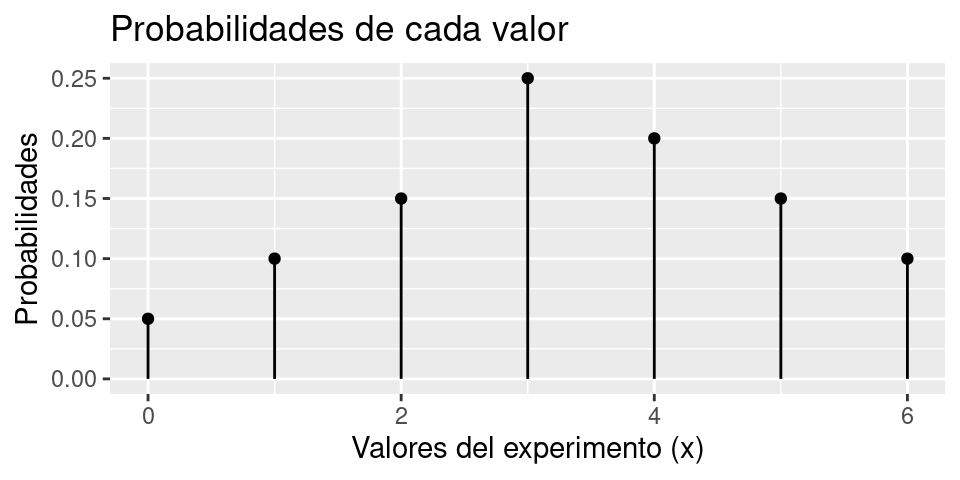
\includegraphics{estadisticas_files/figure-latex/plotmasa-1} 

}

\caption{Función de masa}\label{fig:plotmasa}
\end{figure}

Cabe mencionar que cualquier función de masa de probabilidad requiere cumplir las siguientes condiciones

\begin{enumerate}
\def\labelenumi{\arabic{enumi}.}
\tightlist
\item
  \(p(x) > 0, \forall x \in X\)
\item
  \(\displaystyle\sum_{\text{todas las x posibles}} p(x) = 1\)
\end{enumerate}

para que se válida.

\begin{exercise}

Seis lotes de componentes están listos para ser enviados por un proveedor. El número de componentes defectuosos en cada lote es como sigue:

\begin{table}[H]
\centering
\begin{tabular}[t]{>{}lclclcl}
\toprule
\textbf{Lote} & 1 & 2 & 3 & 4 & 5 & 6\\
\textbf{Número de defectuosos} & 0 & 2 & 0 & 1 & 2 & 0\\
\bottomrule
\end{tabular}
\end{table}

\end{exercise}

Uno de estos lotes tiene que ser seleccionado al azar para ser enviado a un cliente particular. Sea \(X\) el número de componentes defectuosos en el lote seleccionado. Los tres posibles valores de \(X\) son 0, 1 y 2.

\begin{enumerate}
\def\labelenumi{\alph{enumi}.}
\tightlist
\item
  Determine los la probabilidad para cada uno de los valores de \(X\). Interprete.
\item
  Verifique las condiciones de la función de masa de probabilidad asociada al experimento.
\item
  Grafique la función de masa asociada.
\end{enumerate}

\begin{exercise}
\protect\hypertarget{exr:telefonica}{}\label{exr:telefonica}

Una empresa de ventas en línea dispone de seis líneas telefónicas. Sea \(X\) el número de líneas en uso en un tiempo especificado. Suponga que la función de masa de probabilidad de \(X\) es la que se da en la tabla adjunta.

\begin{table}[H]
\centering
\begin{tabular}[t]{cccccccc}
\toprule
$x$ & 0 & 1 & 2 & 3 & 4 & 5 & 6\\
$p(x)$ & 0.1 & 0.15 & 0.2 & 0.25 & 0.2 & 0.06 & 0.04\\
\bottomrule
\end{tabular}
\end{table}

Grafique la función de masa asociada, y luego calcule la probabilidad de cada uno de los siguientes eventos.

\begin{enumerate}
\def\labelenumi{\alph{enumi}.}
\tightlist
\item
  Cuando mucho tres líneas están en uso.
\item
  Menos de tres líneas están en uso.
\item
  Por lo menos tres líneas están en uso.
\item
  Entre dos y cinco líneas, inclusive, están en uso.
\item
  Entre dos y cuatro líneas, inclusive, no está en uso.
\item
  Por lo menos cuatro líneas no están en uso.
\end{enumerate}

\end{exercise}

\subsection{Función de distribución acumulada}\label{funciuxf3n-de-distribuciuxf3n-acumulada}

Para algún valor fijo de \(x\), a menudo se desea calcular la probabilidad de que el valor observado de \(X\) sea cuando mucho \(x\) (\(X \leq x\)). Por ejemplo, consideremos la siguiente función de masa.

\begin{equation}
\notag
\begin{split}
P(X = x) = p(x) = \left\lbrace
\begin{matrix}
0.5 & x = 0\\
0.167 & x = 1\\
0.333 & x = 2\\
0 & \text{en otro caso}\\
\end{matrix}
\right.
\end{split}
\end{equation}

La probabilidad de que \(X\) sea cuando mucho de 1 es entonces

\[P(X \leq 1) = p(0) + p(1) = 0.5 + 0.167 = 0.667\]
Asimismo,

\[P(X \leq 0) = P(X = 0) = 0.5.\]

La \textbf{función de distribución acumulada} (fda) \(F(x)\) de una variable aleatoria discreta \(X\) con función de masa de probabilidad \(P(X=x)\) se define como

\begin{equation}
F(x) = P(X\leq x) =\displaystyle\sum_{y\leq x}P(X=y)
\label{eq:fdadiscreta}
\end{equation}

Para cualquier número \(x\), \(F(X)\) es la probabilidad de que el valor observado de \(X\) será cuando mucho (como máximo) \(x\). \citep[página 95]{Devore}

\begin{example}
Consideremos un grupo de cinco donadores de sangre potenciales, \(a, b, c, d\) y \(e\), de los cuales solo \(a\) y \(b\) tienen sangre tipo O+. Se determinará en orden aleatorio el tipo de sangre con cinco muestras, una de cada individuo hasta que se identifique un individuo O+. Sea la variable aleatoria \(Y =\) \emph{el número de exámenes de sangre para identificar un individuo O+}. Entonces la función de masa de probabilidad de \(Y\) es

\begin{table}[H]
\centering
\begin{tabular}[t]{ccccc}
\toprule
$y$ & 1 & 2 & 3 & 4\\
$p(y)$ & 0.4 & 0.3 & 0.2 & 0.1\\
\bottomrule
\end{tabular}
\end{table}

Para determinar la función de distribución acumulada \(F(Y)\), lo primero es determinar el valor de \(F(Y)\) para cada uno de los valores posibles del conjunto (\(1,2,3,4\)):

\begin{equation}
\notag
\begin{split}
F(1) &= P(Y\leq 1) = P(Y = 1) = p(1) = 0.4\\
F(2) &= P(Y\leq 2) = P(Y = 1 \text{ o } 2) = p(1) + p(2) = 0.7\\
F(3) &= P(Y\leq 3) = P(Y = 1 \text{ o } 2 \text{ o } 3) = p(1) + p(2) + p(3) = 0.9\\
F(4) &= P(Y\leq 4) = P(Y = 1 \text{ o } 2 \text{ o } 3 \text{ o } 4) = p(1) + p(2) + p(3) + p(4) = 1\\
\end{split}
\end{equation}

Ahora con cualquier otro número \(y\), \(F(Y)\) será igual al valor de \(F\) con el valor más próximo posible de \(Y\) a la izquierda de \(y\). Por ejemplo, \(F(2.7) = P(Y\leq 2.7) = p(Y\leq 2) = 0.7\) y \(F(3.9999) = F(3) = 0.9\). La función de distribución acumulativa es por lo tanto

\begin{equation}
\notag
\begin{split}
F(y) = \left\lbrace
\begin{matrix}
0 & \text{si } & y < 1\\
0.4 & \text{si } & 1\leq y < 2\\
0.7 & \text{si } & 2\leq y < 3\\
0.9 & \text{si } & 3\leq y < 4\\
1 & \text{si } & y\geq 4\\
\end{matrix}
\right.
\end{split}
\end{equation}

La siguiente figura muestra la gráfica de \(F(y)\).

\begin{Shaded}
\begin{Highlighting}[]
\NormalTok{df }\OtherTok{=} \FunctionTok{data.frame}\NormalTok{(}\StringTok{"y"} \OtherTok{=} \DecValTok{1}\SpecialCharTok{:}\DecValTok{4}\NormalTok{, }\CommentTok{\# Valores de Y}
                \StringTok{"p"} \OtherTok{=} \FunctionTok{c}\NormalTok{(}\FloatTok{0.4}\NormalTok{,}\FloatTok{0.7}\NormalTok{,}\FloatTok{0.9}\NormalTok{,}\DecValTok{1}\NormalTok{)) }\CommentTok{\# Probabilidades acumuladas asociadas}
\FunctionTok{ggplot}\NormalTok{( }\CommentTok{\# Ambiente gráfico}
  \AttributeTok{data =}\NormalTok{ df, }\CommentTok{\# Base de datos}
  \FunctionTok{aes}\NormalTok{(}\AttributeTok{x =}\NormalTok{ y, }\CommentTok{\# NOmbre de la variable a graficar en el eje X}
      \AttributeTok{y =}\NormalTok{ p)) }\SpecialCharTok{+} \CommentTok{\# Nombre de la variable a graficar en el eje Y}
  \FunctionTok{geom\_segment}\NormalTok{( }\CommentTok{\# Generar segmentos}
    \FunctionTok{aes}\NormalTok{(}\AttributeTok{x =} \FunctionTok{c}\NormalTok{(}\FunctionTok{min}\NormalTok{(y),y[}\SpecialCharTok{{-}}\FunctionTok{length}\NormalTok{(y)]), }\CommentTok{\# Coordenada X de puntos de inicio de los segmentos}
        \AttributeTok{y =} \FunctionTok{c}\NormalTok{(}\FunctionTok{min}\NormalTok{(y),p[}\SpecialCharTok{{-}}\FunctionTok{length}\NormalTok{(y)]), }\CommentTok{\# Coordenada Y de puntos de inicio de los segmentos}
        \AttributeTok{xend =} \FunctionTok{c}\NormalTok{(}\FunctionTok{min}\NormalTok{(y),y[}\SpecialCharTok{{-}}\DecValTok{1}\NormalTok{]), }\CommentTok{\# Coordenada X de puntos finales de los segmentos}
        \AttributeTok{yend =} \FunctionTok{c}\NormalTok{(}\FunctionTok{min}\NormalTok{(y),p[}\SpecialCharTok{{-}}\FunctionTok{length}\NormalTok{(y)]))) }\SpecialCharTok{+} \CommentTok{\# Coordenada X de puntos finales de los segmentos}
  \FunctionTok{geom\_segment}\NormalTok{( }\CommentTok{\# Código que genera la flecha dentro del gráfico}
    \FunctionTok{aes}\NormalTok{(}\AttributeTok{x =}\NormalTok{ y[}\FunctionTok{length}\NormalTok{(y)],}
        \AttributeTok{y =}\NormalTok{ p[}\FunctionTok{length}\NormalTok{(y)],}
        \AttributeTok{xend =}\NormalTok{ y[}\FunctionTok{length}\NormalTok{(y)] }\SpecialCharTok{+} \FunctionTok{mean}\NormalTok{(y[}\DecValTok{2}\SpecialCharTok{:}\FunctionTok{length}\NormalTok{(y)]}\SpecialCharTok{{-}}\NormalTok{ y[}\DecValTok{1}\SpecialCharTok{:}\FunctionTok{length}\NormalTok{(y)}\SpecialCharTok{{-}}\DecValTok{1}\NormalTok{]),}
        \AttributeTok{yend =}\NormalTok{ p[}\FunctionTok{length}\NormalTok{(y)]),}
    \AttributeTok{arrow =} \FunctionTok{arrow}\NormalTok{(}\AttributeTok{length =} \FunctionTok{unit}\NormalTok{(}\FloatTok{0.2}\NormalTok{, }\StringTok{"cm"}\NormalTok{)), }\CommentTok{\# Argumento que permite dar la forma de flecha al último segmento}
    \AttributeTok{alpha =} \FloatTok{0.4}\NormalTok{) }\SpecialCharTok{+}
  \FunctionTok{geom\_point}\NormalTok{(}\AttributeTok{col =} \StringTok{"darkred"}\NormalTok{) }\SpecialCharTok{+} \CommentTok{\# Punto de incio de los segmentos}
  \FunctionTok{scale\_y\_continuous}\NormalTok{(}\AttributeTok{limits =} \FunctionTok{c}\NormalTok{(}\DecValTok{0}\NormalTok{,}\DecValTok{1}\NormalTok{)) }\SpecialCharTok{+} \CommentTok{\# Edición de los límites del eje Y}
  \FunctionTok{labs}\NormalTok{( }\CommentTok{\# Edición de títulos}
    \AttributeTok{title =} \StringTok{"Probabilidad acumulada"}\NormalTok{, }\CommentTok{\# Título del gráfico}
    \AttributeTok{x =} \StringTok{"Valores de y"}\NormalTok{, }\CommentTok{\# Título del eje X}
    \AttributeTok{y =} \StringTok{"F(y)"}\NormalTok{) }\CommentTok{\# Título del eje Y}
\end{Highlighting}
\end{Shaded}

\begin{figure}

{\centering 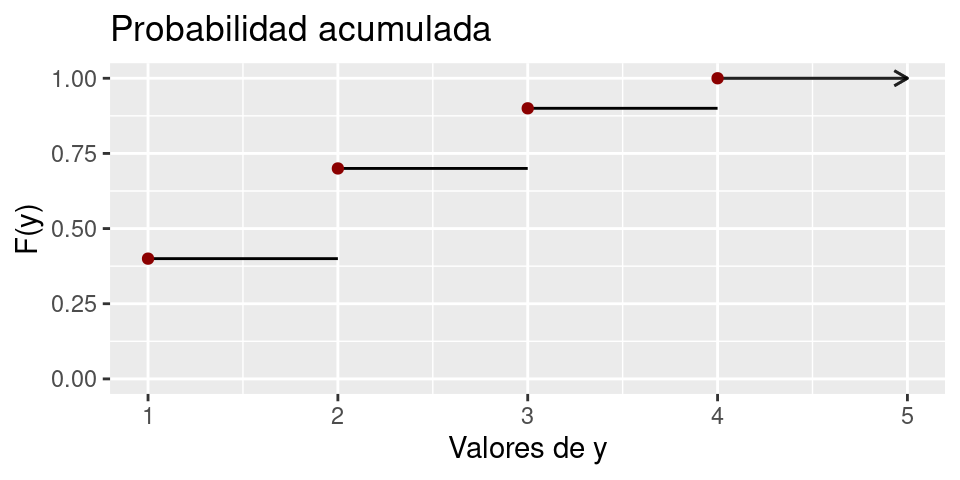
\includegraphics{estadisticas_files/figure-latex/unnamed-chunk-37-1} 

}

\caption{Función de distribución acumulada}\label{fig:unnamed-chunk-37}
\end{figure}

Para una variable aleatorio discreta \(X\), la gráfica de \(F(X)\) mostrará un saltó con cada valor posible de \(X\) y será plana entre los valores posibles. Tal gráfica se conoce como función escalonada.
\end{example}

Una propiedad que surge de la función de distribución acumulada es que, para dos números cualesquiera \(a\) y \(b\) con \(a\leq b\).

\begin{equation}
P(a\leq X \leq b) = P(X \leq b) - P(X < a)
\label{eq:fda2}
\end{equation}

En caso de que se desee calcular \(P(a < X \leq b)\), la propiedad sería

\begin{equation}
P(a < X \leq b) = P(X \leq b) - P(X \leq a) = F(a) - F(b)
\label{eq:fda3}
\end{equation}

De lo anterior se deduce, que dependiendo de los signos de desigualdad, cambiará la forma en la se escribe la propiedad.

\begin{exercise}
Remítase al ejercicio \ref{exr:telefonica} y calcule y trace la gráfica de la función de distribución acumulada \(F(X)\). Luego, utilícela para calcular las probabilidades de los eventos dados en los ítem a. y d.~de dicho problema. Además, grafique la función de distribución acumulada.
\end{exercise}

\begin{exercise}

Una organización de protección al consumidor que habitualmente evalúa automóviles nuevos reporta el número de defectos importantes encontrados en un carro seleccionado al azar de cierto tipo. La función de distribución acumulativa de \(Y\) es la siguiente.

\begin{equation}
\notag
\begin{split}
F(y) = \left\lbrace
\begin{matrix}
0 & \text{si } & y < 0\\
0.06 & \text{si } & 0\leq y < 1\\
0.19 & \text{si } &  1\leq y < 2\\
0.39 & \text{si } & 2\leq y < 3\\
0.67 & \text{si } & 3\leq y < 4\\
0.92 & \text{si } & 4\leq y < 5\\
0.97 & \text{si } & 5\leq y < 6\\
1 & \text{si } & y\geq 6\\
\end{matrix}
\right.
\end{split}
\end{equation}

\begin{enumerate}
\def\labelenumi{\arabic{enumi}.}
\item
  Calcule las siguientes probabilidades directamente con la función de distribución acumulada:

  \begin{enumerate}
  \def\labelenumii{\alph{enumii}.}
  \tightlist
  \item
    \(p(2)\), es decir, \(P(Y=2)\)
  \item
    \(P(Y>3)\)
  \item
    \(P(2\leq Y\leq 5)\)
  \item
    \(P(2 < Y < 5)\)
  \end{enumerate}
\item
  ¿Cuál es la función de masa de probabilidad de \(X\)? Grafique la función de masa de probabilidad, y la función de distribución acumulada.
\end{enumerate}

\end{exercise}

\begin{exercise}

En una fábrica de productos electrónicos, se sabe que la probabilidad de que un artículo sea defectuoso sigue una distribución de probabilidad de masa con los siguientes valores:

\begin{table}[H]
\centering
\begin{tabular}[t]{cc}
\toprule
Número de defectos & Probabilidad\\
\midrule
0 & 0.50\\
1 & 0.30\\
2 & 0.02\\
3 & 0.08\\
4 & 0.10\\
\bottomrule
\end{tabular}
\end{table}

A continuación:

\begin{enumerate}
\def\labelenumi{\arabic{enumi}.}
\tightlist
\item
  Determine la función de masa de probabilidad.
\item
  Determine la función de distribución acumulada.
\item
  Si se selecciona un artículo al azar. Utilizando la función de distribución acumulada calcule:

  \begin{enumerate}
  \def\labelenumii{\alph{enumii}.}
  \tightlist
  \item
    La probabilidad de que tenga cuando mucho de 2 defectos.
  \item
    La probabilidad de que tenga más de 0.4 defectos.
  \item
    La probabilidad de que tenga entre 1 y 4 defectos.
  \item
    La probabilidad de que tenga cuando menos 2.7 defectos.
  \end{enumerate}
\end{enumerate}

\end{exercise}

\subsection{Distribuciones}\label{distribuciones}

A continuación, se dan a conocer algunas de las distribución de probabilidad discreta más utilizadas. Cabe mencionar, que existen muchas otras distribuciones, por lo que se invita al estudiante a informarse de ellas en caso de que lo requiera.

\subsubsection{Uniforme}\label{uniforme}

El ejemplo más sencillo de de una distribución de probabilidad discreta dada mediante una fórmula es la \textbf{distribución uniforme discreta} \citep[página 191]{anderson}. Su función de masa de probabilidad está definida por

\begin{equation}
P(X=x) = \dfrac{1}{n}
\label{eq:uniformediscreta}
\end{equation}

donde

\[n = \text{número de valores que puede tomar la variable aleatoria.}\]

\begin{example}
Consideremos el experimento de lanzar un dado de seis caras. Se define la variable aleatoria \(X\) como el número de puntos en la cara del dado que cae hacia arriba. En este experimento la variable aleatoria toma 6 valores posibles (\(n = 6\)). Por lo tanto, la función de masa de probabilidad de esta variable aleatoria uniforme discreta es

\[P(X = x)=1/6 \text{, } x = 1,2,3,4,5,6\]
\end{example}

La figura \ref{fig:simUD}, muestra una simulación de la función de masa de probabilidad de la distribución uniforme discreta, dependiendo del número de valores que puede tomar la variable aleatoria (\(n\)).

\begin{figure}

{\centering 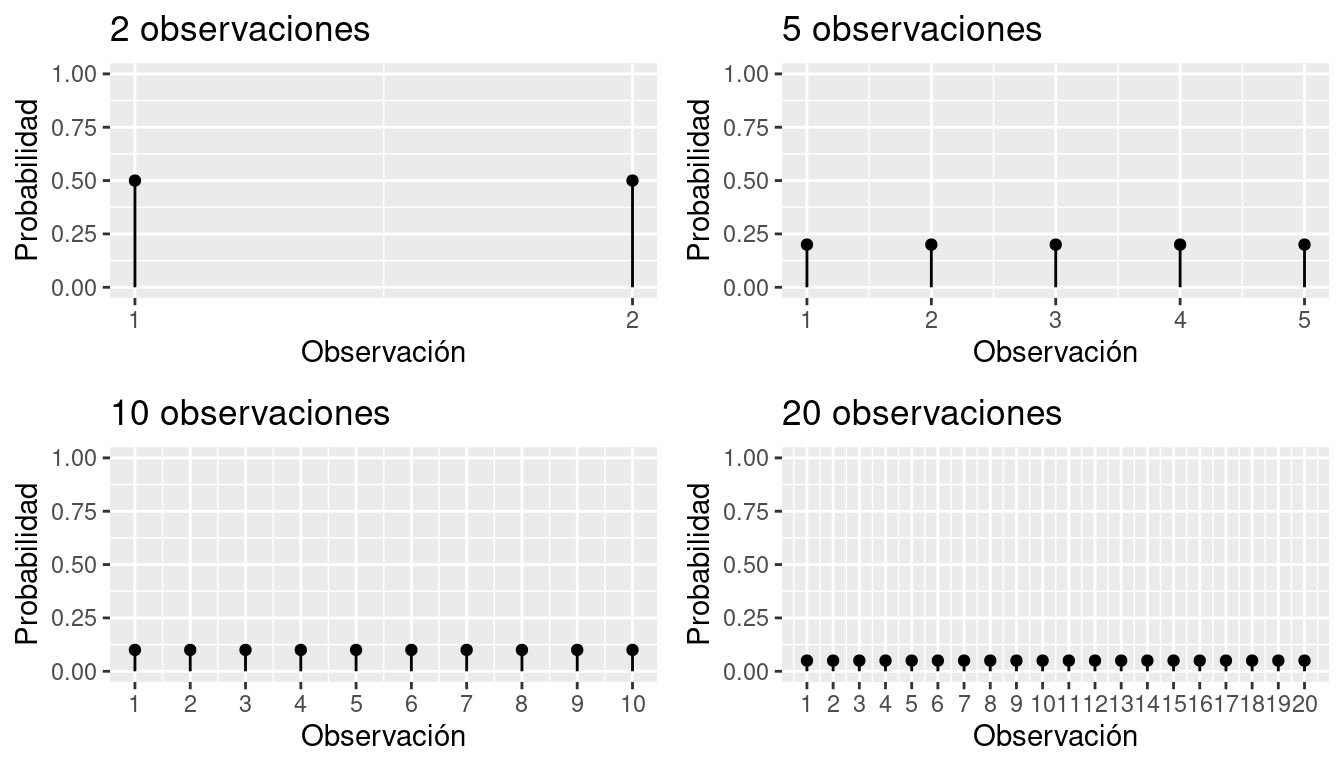
\includegraphics{estadisticas_files/figure-latex/simUD-1} 

}

\caption{Simulación de la distribución Uniforme discreta}\label{fig:simUD}
\end{figure}

\subsubsection{Bernoulli}\label{bernoulli}

La distribución Bernoulli es una distribución de probabilidad discreta que describe el resultado de un experimento de ensayo único que puede tener dos posibles resultados, a menudo etiquetados como éxito y fracaso, con una probabilidad de éxito de \(p\) y una probabilidad de fracaso de \(q = 1 - p\). La función de masa de probabilidad de la distribución Bernoulli está dada por:

\begin{equation}
P(X = x) = p^x(1-p)^{1-x}
\label{eq:bernoulli}
\end{equation}

donde \(x\) puede tomar únicamente los valores de 0 y 1 \citep[página 105]{larsen}.

La figura \ref{fig:simBer}, muestra una simulación de la función de masa de probabilidad de la distribución Bernoulli, dependiendo de la probabilidad de éxito (\(p\)).

\begin{figure}

{\centering 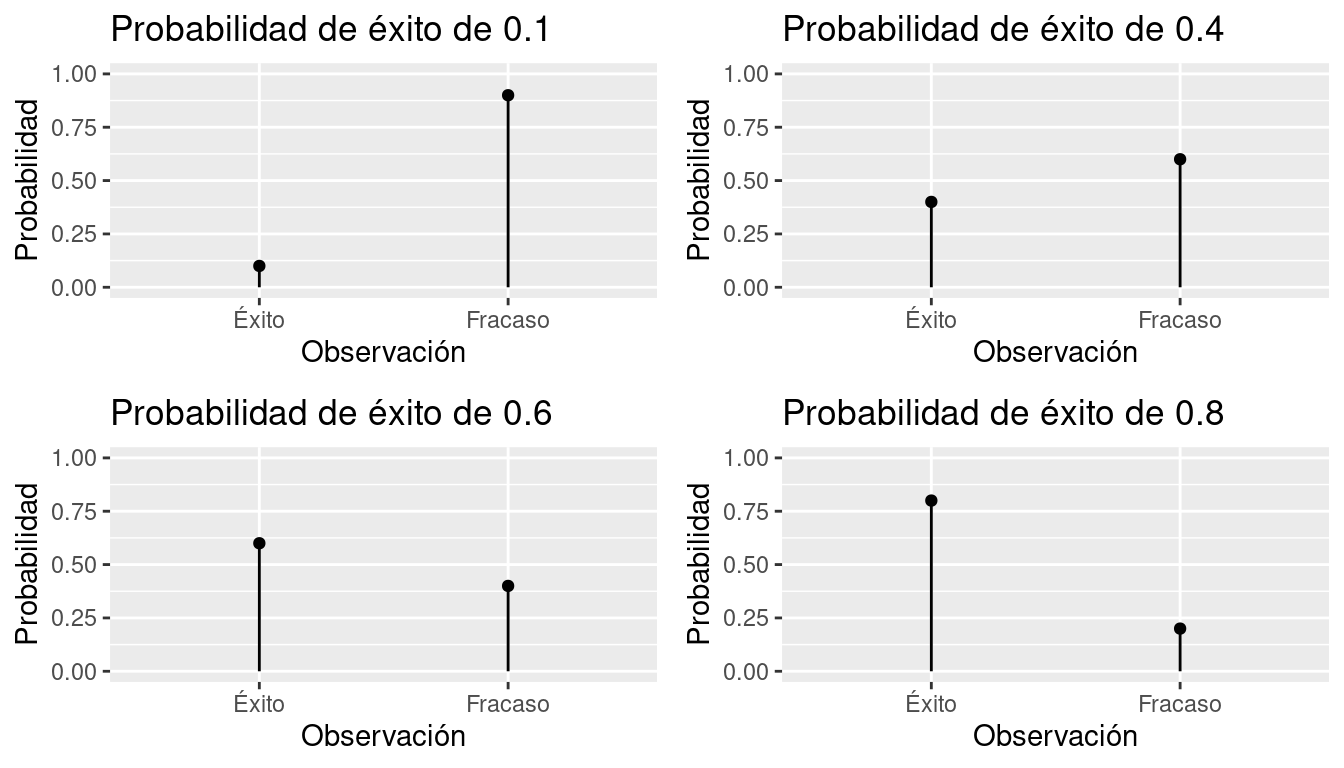
\includegraphics{estadisticas_files/figure-latex/simBer-1} 

}

\caption{Simulación de la distribución Binomial}\label{fig:simBer}
\end{figure}

\begin{example}

En un experimento de lanzamiento de moneda, se puede modelar la probabilidad de obtener cara como una distribución Bernoulli. En este caso, si se define ``éxito'' como obtener cara y ``fracaso'' como obtener sello, entonces la probabilidad de éxito es \(p = 0.5\) y la probabilidad de fracaso es \(q = 1 - p = 0.5\). Entonces, la distribución Bernoulli para este experimento estaría dada por:

\begin{itemize}
\tightlist
\item
  \(P(\text{Obtener cara}) = p = 0.5\)
\item
  \(P(\text{Obtener sello}) = q = 0.5\)
\end{itemize}

\end{example}

\begin{example}

En una campaña publicitaria en línea, se puede modelar la probabilidad de que un usuario haga clic en un anuncio como una distribución Bernoulli. En este caso, si se define ``éxito'' como un usuario que hace clic en el anuncio y ``fracaso'' como un usuario que no hace clic, entonces la probabilidad de éxito es p y la probabilidad de fracaso es \(q = 1 - p\). Supongamos que la probabilidad de que un usuario haga clic en el anuncio es del 10\%, es decir, \(p = 0.1\). Entonces, la distribución Bernoulli para este experimento estaría dada por:

\begin{itemize}
\tightlist
\item
  \(P(\text{Hacer clic en el anuncio}) = p = 0.1\)
\item
  \(P(\text{No hacer clic en el anuncio}) = q = 0.9\)
\end{itemize}

\end{example}

\subsubsection{Binomial}\label{binomial}

La distribución de probabilidad binomial es una distribución de probabilidad que tiene muchas aplicaciones. Está relacionada con un experimento de pasos múltiples al que se llama experimento binomial \citep[paǵina 200]{anderson}.

Un experimento binomial tiene las siguientes cuatro propiedades.

\begin{enumerate}
\def\labelenumi{\arabic{enumi}.}
\tightlist
\item
  El experimento consiste en una serie de n ensayos idénticos.
\item
  En cada ensayo hay dos resultados posibles. A uno de estos resultados se le llama éxito y al otro se le llama fracaso.
\item
  La probabilidad de éxito, que se denota \(p\), no cambia de un ensayo a otro. Por ende, la probabilidad de fracaso, que se denota \(1 - p\), tampoco cambia de un ensayo a otro.
\item
  Los ensayos son independientes.
\end{enumerate}

Si se presentan las propiedades \(2, 3\) y \(4\), se dice que los ensayos son generados por un proceso de Bernoulli. Si, además, se presenta la propiedad 1, se trata de un experimento binomial.

En un experimento binomial lo que interesa es el número de éxitos en n ensayos. Si \(X\) denota el número de éxitos en \(n\) ensayos, es claro que \(x\) tomará los valores \(0, 1, 2, 3, \ldots, n\). Dado que el número de estos valores es finito, \(X\) es una variable aleatoria discreta. A la distribución de probabilidad correspondiente a esta variable aleatoria se le llama \textbf{distribución de probabilidad binomial}.

\begin{example}
Considere el experimento que consiste en lanzar una moneda cinco veces y observar si la cara de la moneda que cae hacia arriba es cara o cruz. Suponga que se desea contar el número de caras que aparecen en los cinco lanzamientos. ¿Presenta este experimento las propiedades de un experimento binomial? ¿Cuál es la variable aleatoria que interesa? Observe que:

\begin{enumerate}
\def\labelenumi{\arabic{enumi}.}
\tightlist
\item
  El experimento consiste en cinco ensayos idénticos; cada ensayo consiste en lanzar una moneda.
\item
  En cada ensayo hay dos resultados posibles: cara o cruz. Se puede considerar cara como éxito y cruz como fracaso.
\item
  La probabilidad de éxito y la probabilidad de fracaso son iguales en todos los ensayos, siendo \(p = 0.5\) y \(1 - p = 0.5\).
\item
  Los ensayos o lanzamientos son independientes porque al resultado de un ensayo no afecta a lo que pase en los otros ensayos o lanzamientos.
\end{enumerate}

Por tanto, se satisfacen las propiedades de un experimento binomial. La variable aleatoria que interesa es \(X =\) número de caras que aparecen en cinco ensayos. En este caso, X puede tomar los valores \(0, 1, 2, 3, 4\) o \(5\).
\end{example}

La función de masa de probabilidad de la distribución Binomial está dada por:

\begin{equation}
P(X = x) = \binom{n}{x}p^x(1-p)^{n-x}
\label{eq:binomial}
\end{equation}

donde

\begin{equation}
\notag
\begin{split}
P(X = x) &= \text{probabilidad de } x \text{ éxitos en } n \text{ ensayos}\\
n &= \text{ número de ensayos}\\
\binom{n}{x} &= \dfrac{n!}{x!(n-x)!}\\
p &= \text{probabilidad de un éxito en cualquiera de los ensayos}\\
1 - p &= \text{probabilidad de un fracaso en cualquiera de los ensayos}\\
\end{split}
\end{equation}

La figura \ref{fig:simBinomial}, muestra una simulación de la función de masa de probabilidad de la distribución Binomial, dependiendo del número de ensayos (\(n\)) y de la probabilidad de éxito (\(p\)).

\begin{figure}

{\centering 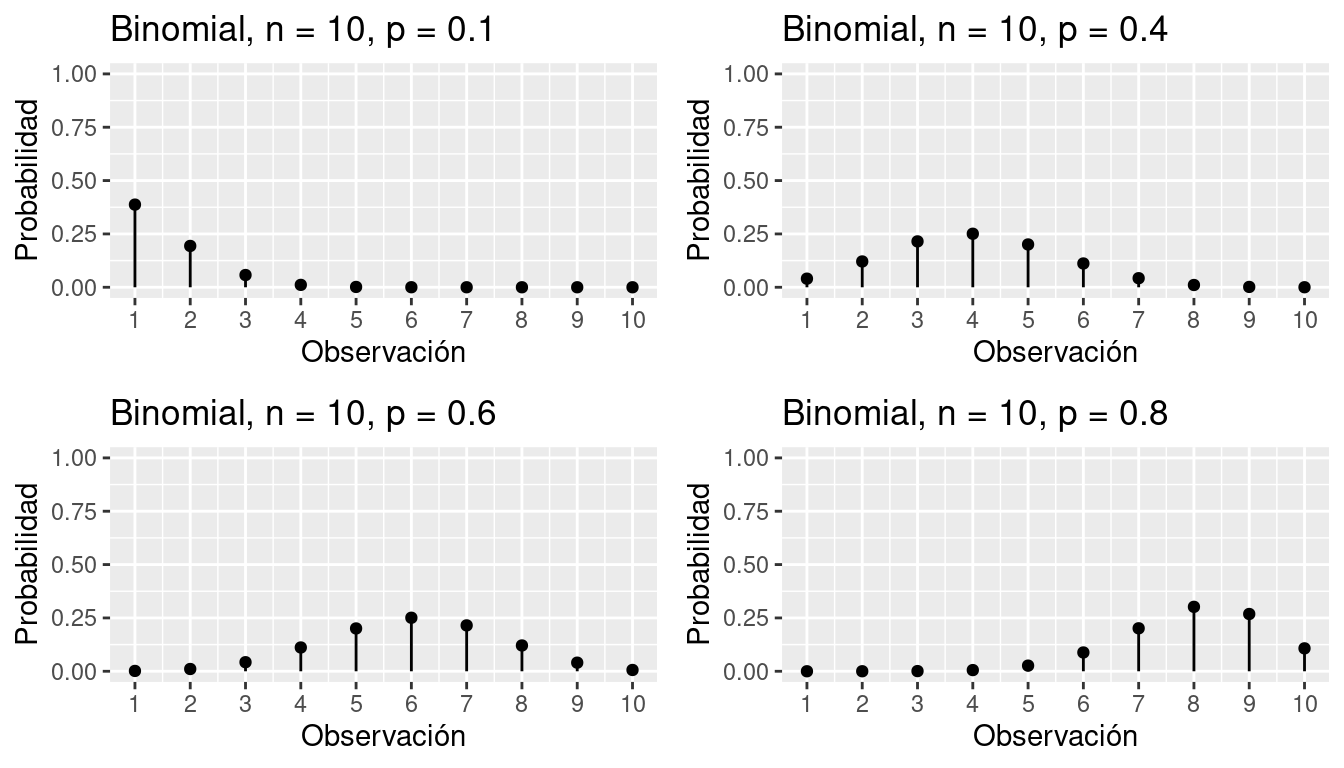
\includegraphics{estadisticas_files/figure-latex/simBinomial-1} 

}

\caption{Simulación de la distribución Binomial}\label{fig:simBinomial}
\end{figure}

\begin{example}
\protect\hypertarget{exm:ejcomandosbin}{}\label{exm:ejcomandosbin}

Considere una distribución Binomial con \(n = 7\) y \(p = 0.2\).

\begin{enumerate}
\def\labelenumi{\alph{enumi}.}
\item
  Escriba la función de masa de probabilidad asociada.

  \begin{equation}
  \notag
  P(X=x) = \binom{7}{x}0.2^x(1-0.2)^{7-x}
  \end{equation}
\item
  Calcule \(p(4)\).

  Recordemos que \(p(4) = P(X = 4)\). Para poder calcular probabilidades en un punto exacto (igual a 4) en R, se debe usar el prefijo \emph{d} seguido de la abreviatura de la distribución discreta, en este caso la abreviatura de la distribución Binomial es \emph{binom}.

\begin{Shaded}
\begin{Highlighting}[]
\FunctionTok{dbinom}\NormalTok{(}
  \AttributeTok{x =} \DecValTok{4}\NormalTok{, }\CommentTok{\# Valor de X para el cual se desea calcular la probabilidad}
  \AttributeTok{size =} \DecValTok{7}\NormalTok{, }\CommentTok{\# Cantidad de ensayos}
  \AttributeTok{prob =} \FloatTok{0.2}\NormalTok{, }\CommentTok{\# Probabilidad de éxito}
\NormalTok{)}
\end{Highlighting}
\end{Shaded}

\begin{verbatim}
## [1] 0.028672
\end{verbatim}

  Por lo tanto, la probabilidad de obtener 4 resultados exitosos de 7 ensayos es de 0.028672.
\item
  Calcule \(P(X\leq 2)\).

  En R para poder calcular probabilidades acumuladas es posible usar el prefijo \emph{p} seguido de la abreviatura de la distribución discreta, en este caso la abreviatura de la distribución Binomial es \emph{binom}.

  Por defecto, R considera que las probabilidades acumuladas son del tipo \(P(X \leq x)\), tal como se presenta en este enunciado.

\begin{Shaded}
\begin{Highlighting}[]
\FunctionTok{pbinom}\NormalTok{(}
  \AttributeTok{q =} \DecValTok{2}\NormalTok{, }\CommentTok{\# Se consideran valores MENORES o iguales a 2}
  \AttributeTok{size =} \DecValTok{7}\NormalTok{, }\CommentTok{\# Cantidad de ensayos}
  \AttributeTok{prob =} \FloatTok{0.2}\NormalTok{, }\CommentTok{\# Probabilidad de éxito}
\NormalTok{)}
\end{Highlighting}
\end{Shaded}

\begin{verbatim}
## [1] 0.851968
\end{verbatim}

  Por lo tanto, la probabilidad de obtener 2 o menos resultados exitosos de 7 ensayos es de 0.85.
\item
  Calcule \(P(X < 5)\).

  En este caso antes de calcular en la probabilidad en R, se debe transformar la expresión a la forma \(P(X \leq x)\). Ya que estamos trabajando con eventos discretos, tenemos que

  \[P(X < 5) = P(X \leq 4)\]

  Luego, esta probabilidad la podemos calcular en R de la siguiente manera.

\begin{Shaded}
\begin{Highlighting}[]
\FunctionTok{pbinom}\NormalTok{(}
  \AttributeTok{q =} \DecValTok{4}\NormalTok{, }\CommentTok{\# Se consideran valores MENORES o iguales a 4}
  \AttributeTok{size =} \DecValTok{7}\NormalTok{, }\CommentTok{\# Cantidad de ensayos}
  \AttributeTok{prob =} \FloatTok{0.2}\NormalTok{, }\CommentTok{\# Probabilidad de éxito}
\NormalTok{)}
\end{Highlighting}
\end{Shaded}

\begin{verbatim}
## [1] 0.995328
\end{verbatim}

  Por lo tanto, la probabilidad de obtener menos de 5 resultados exitosos de 7 ensayos es de 0.99.
\item
  Calcule \(P(X > 1)\).

  R incluye un comando para aquellos casos en los que el signo de desigualdad estricto es del tipo mayor.

\begin{Shaded}
\begin{Highlighting}[]
\FunctionTok{pbinom}\NormalTok{(}
  \AttributeTok{q =} \DecValTok{1}\NormalTok{, }\CommentTok{\# Se consideran valores MAYORES o iguales a 1}
  \AttributeTok{size =} \DecValTok{7}\NormalTok{, }\CommentTok{\# Cantidad de ensayos}
  \AttributeTok{prob =} \FloatTok{0.2}\NormalTok{, }\CommentTok{\# Probabilidad de éxito}
  \AttributeTok{lower.tail =} \ConstantTok{FALSE} \CommentTok{\# En caso de que se tenga el signo mayor estricto}
\NormalTok{)}
\end{Highlighting}
\end{Shaded}

\begin{verbatim}
## [1] 0.4232832
\end{verbatim}

  Por lo tanto, la probabilidad de obtener más de 1 resultado exitoso de 7 ensayos es de 0.42.
\item
  Calcule \(P(X \geq 1)\).

  Para aquellos casos en que se tenga el signo de mayor igual (\(\geq\)), lo más más recomendable es transformar la expresión a estricto (\(>\)) para así utilizar un código similar al del ejemplo \emph{d.}. Ya que estamos trabajando con eventos discretos, tenemos que

  \[P(X \geq 1) = P(X > 0)\]

  Luego, esta probabilidad la podemos calcular en R de la siguiente manera.

\begin{Shaded}
\begin{Highlighting}[]
\FunctionTok{pbinom}\NormalTok{(}
  \AttributeTok{q =} \DecValTok{0}\NormalTok{, }\CommentTok{\# Se consideran valores MAYORES a 0}
  \AttributeTok{size =} \DecValTok{7}\NormalTok{, }\CommentTok{\# Cantidad de ensayos}
  \AttributeTok{prob =} \FloatTok{0.2}\NormalTok{, }\CommentTok{\# Probabilidad de éxito}
  \AttributeTok{lower.tail =} \ConstantTok{FALSE} \CommentTok{\# En caso de que se tenga el signo mayor estricto}
\NormalTok{  )}
\end{Highlighting}
\end{Shaded}

\begin{verbatim}
## [1] 0.7902848
\end{verbatim}

  Por lo tanto, la probabilidad de obtener al menos 1 resultado exitoso de 7 ensayos es de 0.79.
\item
  ¿Para que valor de \(x\), \(P(X \leq x) = 0.6\)?

  Despejar esta ecuación puede llegar a ser engorroso. Sin embargo, R posee un argumento para determinar estos valores. Para el calculo se debe usar el prefijo \emph{q} seguido de la abreviatura de la distribución discreta, en este caso la abreviatura de la distribución Binomial es \emph{binom}.

\begin{Shaded}
\begin{Highlighting}[]
\FunctionTok{qbinom}\NormalTok{(}
  \AttributeTok{p =} \FloatTok{0.6}\NormalTok{, }\CommentTok{\# Valor resultante de la probabilidad}
  \AttributeTok{size =} \DecValTok{7}\NormalTok{, }\CommentTok{\# Cantidad de ensayos}
  \AttributeTok{prob =} \FloatTok{0.2}\NormalTok{, }\CommentTok{\# Probabilidad de éxito}
\NormalTok{  )}
\end{Highlighting}
\end{Shaded}

\begin{verbatim}
## [1] 2
\end{verbatim}

  Por lo tanto, para \(x = 2\), la probabilidad de obtener a lo más \(x\) resultados exitosos es de 0.6.
\end{enumerate}

\end{example}

\begin{example}
Un acusado va a ser declarado inocente o culpable por un jurado popular. Para ser condenado es necesario que al menos 7 personas de las 10 del jurado voten culpable. Dado que en los programas de televisión ya han dado muchos detalles del caso, los miembros del jurado están atendiendo \textit{twitter} o leyendo el diario en vez de escuchar al fiscal y al abogado, porque van a decidir tirando una moneda al aire. ¿Cuál es la probabilidad de que el acusado sea declarado inocente?

La probabilidad de éxito (inocencia) es de \(p = 0.5\). Sea \(X\) el número éxitos (votos de inocencia) en 10 ensayos (votos del jurado). Entonces, la probabilidad de ser declarado inocente esta dada por la siguiente expresión.

\[
P(X \geq 4) = \sum_{k=4}^{10} \binom{10}{k} 0.5^{k}(1-0.5)^{10-k} = 0.82,\text{ o}
\]

Antes de realizar el cálculo en R lo recomendable es transformar la expresión para utilizar el comando adecuado. En este caso, la expresión es:

\[P(X\geq 4) = P(X > 3)\]
Luego, en R.

\begin{Shaded}
\begin{Highlighting}[]
\FunctionTok{pbinom}\NormalTok{(}
  \AttributeTok{q =} \DecValTok{3}\NormalTok{, }\CommentTok{\# Se consideran valores MAYORES o iguales a 3 (es decir, mayor o igual a 4)}
  \AttributeTok{size =} \DecValTok{10}\NormalTok{, }\CommentTok{\# Cantidad de ensayos}
  \AttributeTok{prob =} \FloatTok{0.5}\NormalTok{, }\CommentTok{\# Probabilidad de éxito}
  \AttributeTok{lower.tail =} \ConstantTok{FALSE} \CommentTok{\# TRUE: menor igual, FALSE: mayor estricto}
\NormalTok{)}
\end{Highlighting}
\end{Shaded}

\begin{verbatim}
## [1] 0.828125
\end{verbatim}

Por otro lado, la probabilidad \(P(X\geq 4)\) puede ser escrita como \(1 - P(X \leq 3)\).

\[
1 - P(X \leq 3) = \sum_{k=0}^{3} \binom{10}{k} 0.5^{k}(1-0.5)^{10-k} = 0.82
\]

Es posible calcular esta expresión en R de la siguiente manera.

\begin{Shaded}
\begin{Highlighting}[]
\DecValTok{1} \SpecialCharTok{{-}} \FunctionTok{pbinom}\NormalTok{(}
  \AttributeTok{q =} \DecValTok{3}\NormalTok{, }\CommentTok{\# Se consideran valores MENORES o iguales a 3}
  \AttributeTok{size =} \DecValTok{10}\NormalTok{, }\CommentTok{\# Cantidad de ensayos}
  \AttributeTok{prob =} \FloatTok{0.5} \CommentTok{\# Probabilidad de éxito}
\NormalTok{)}
\end{Highlighting}
\end{Shaded}

\begin{verbatim}
## [1] 0.828125
\end{verbatim}

Por lo tanto, la probabilidad de que el acusado sea declarado inocente es de 0.82.
\end{example}

\begin{exercise}

En una planta de revisión técnica, resulta rechazado el \(42 \%\) de los vehículos livianos. En la primera media hora de un día cualquiera se alcanzan a revisar 9 vehículos.

\begin{enumerate}
\def\labelenumi{\arabic{enumi}.}
\tightlist
\item
  ¿cuál es la probabilidad de que más de 3 sean rechazados?
\item
  ¿cuál es la probabilidad de que a lo más 5 sean rechazados?
\item
  ¿cuál es la probabilidad de que menos de 2 sean rechazados?
\item
  ¿cuál es la probabilidad de no se rechacen todos los vehículos?
\end{enumerate}

\end{exercise}

\begin{exercise}
Se sabe que la probabilidad de que una empresa no pase la revisión de fraude fiscal es de 0.21. De las siguientes 345 empresas que se revisan en búsqueda de fraude fiscal, calcule la probabilidad de que cuando mucho 85 empresas no aprueben la revisión.
\end{exercise}

\begin{exercise}

Un banco sabe que el 8\% de sus clientes no pagan a tiempo sus tarjetas de crédito. Si el banco emite 2500 tarjetas de crédito,

\begin{enumerate}
\def\labelenumi{\arabic{enumi}.}
\tightlist
\item
  ¿Cuál es la probabilidad de que al menos 200 de ellas pertenezcan a clientes que no pagan a tiempo?
\item
  ¿Qué pasaría con la probabilidad de que al menos 200 de las tarjetas de crédito pertenezcan a clientes que no pagan a tiempo si la tasa de incumplimiento del banco aumenta al 9.2\%?
\item
  ¿Cuál es la probabilidad de que exactamente 250 de las tarjetas de crédito pertenezcan a clientes que no pagan a tiempo?
\item
  ¿Cuál es la probabilidad de que cuando mucho 210 de ellas pertenezcan a clientes que no pagan a tiempo?
\end{enumerate}

\end{exercise}

\subsubsection{Poisson}\label{poisson}

Una variable aleatoria discreta que se suele usar para estimar el número de veces que sucede un hecho determinado (ocurrencias) en un intervalo de tiempo o de espacio. Por ejemplo, el número de reparaciones en un autopista o número de fugas en un tubería. Si se satisfacen las siguientes condiciones, el número de ocurrencias es una variable aleatoria discreta definida por la distribución de probabilidad de Poisson \citep[página 211]{anderson}.

\begin{enumerate}
\def\labelenumi{\arabic{enumi}.}
\tightlist
\item
  La probabilidad de ocurrencia es la misma para cualesquiera dos intervalos de la misma magnitud.
\item
  La ocurrencia o no-ocurrencia en cualquier intervalo es independiente de la ocurrencia o no-ocurrencia en cualquier otro intervalo.
\end{enumerate}

La función de masa de probabilidad de Poisson se define mediante la ecuación

\begin{equation}
P(X = x) = \dfrac{\lambda^xe^{-\lambda}}{x!}
\label{eq:poisson}
\end{equation}

en donde

\begin{equation}
\notag
\begin{split}
P(X = x) &= \text{probabilidad de } x \text{ ocurrencias en un intervalo de tiempo}\\
\lambda &= \text{ tasa de ocurrencias en un intervalo}\\
e &\approx 2.71828\\
\end{split}
\end{equation}

Es importante observar, que el número de ocurrencias de \(x\), no tiene límite superior. Esta es un variable aleatoria discreta que toma los valores de una sucesión infinita de números (\(x = 0,1,2,3,4,\ldots\)).

La figura \ref{fig:simPois}, muestra una simulación de la función de masa de probabilidad de la distribución Poisson, dependiendo de la tasa en función del tiempo (\(\lambda\)).

\begin{figure}

{\centering 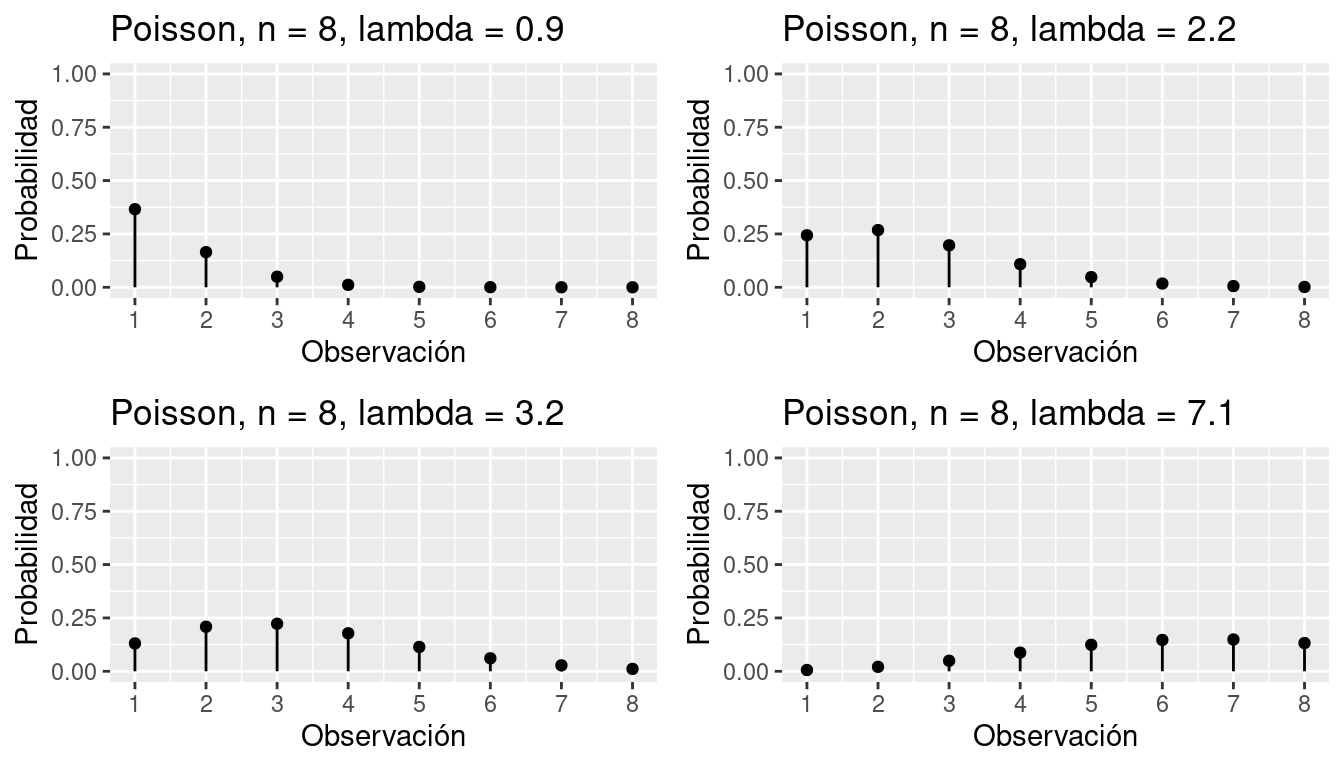
\includegraphics{estadisticas_files/figure-latex/simPois-1} 

}

\caption{Simulación de la distribución Poisson}\label{fig:simPois}
\end{figure}

\begin{example}

Considere una distribución Poisson con \(\lambda = 3\)

\begin{enumerate}
\def\labelenumi{\alph{enumi}.}
\item
  Escriba la función de probabilidad asociada.

  \begin{equation}
  \notag
  P(X=x) = \dfrac{3^xe^{-3}}{x!}
  \end{equation}
\item
  Calcule \(p(2)\).

  Considerando los comandos explicados en el ejemplo \ref{exm:ejcomandosbin}, solo es necesario modificar la abreviatura de la distribución de probabilidad, la cual, en este caso, corresponde a \emph{pois}.

  Recordemos que \(p(2) = P(X = 2)\).

\begin{Shaded}
\begin{Highlighting}[]
\FunctionTok{dpois}\NormalTok{(}
  \AttributeTok{x =} \DecValTok{2}\NormalTok{, }\CommentTok{\# Valor de X para el cual se desea calcular la probabilidad}
  \AttributeTok{lambda =} \DecValTok{3} \CommentTok{\# Tasa de ocurrencia por unidad de tiempo o espacio}
\NormalTok{  )}
\end{Highlighting}
\end{Shaded}

\begin{verbatim}
## [1] 0.2240418
\end{verbatim}

  Por lo tanto, teniendo una tasa de 3 por unidad de tiempo, la probabilidad de que ocurran dos sucesos es de 0.22.
\item
  Calcule \(P(X\leq 3)\).

\begin{Shaded}
\begin{Highlighting}[]
\FunctionTok{ppois}\NormalTok{(}
  \AttributeTok{q =} \DecValTok{3}\NormalTok{, }\CommentTok{\# Valor de X para el cual se desea calcular la probabilidad}
  \AttributeTok{lambda =} \DecValTok{3} \CommentTok{\# Tasa de ocurrencia por unidad de tiempo o espacio}
\NormalTok{  )}
\end{Highlighting}
\end{Shaded}

\begin{verbatim}
## [1] 0.6472319
\end{verbatim}

  Por lo tanto, teniendo una tasa de 3 por unidad de tiempo, la probabilidad de que ocurran a lo más tres sucesos es de 0.64.
\item
  Calcule \(P(X < 2)\).

\begin{Shaded}
\begin{Highlighting}[]
\FunctionTok{ppois}\NormalTok{(}
  \AttributeTok{q =} \DecValTok{1}\NormalTok{, }\CommentTok{\# Valor de X para el cual se desea calcular la probabilidad}
  \AttributeTok{lambda =} \DecValTok{3} \CommentTok{\# Tasa de ocurrencia por unidad de tiempo o espacio}
\NormalTok{  )}
\end{Highlighting}
\end{Shaded}

\begin{verbatim}
## [1] 0.1991483
\end{verbatim}

  Por lo tanto, teniendo una tasa de 3 por unidad de tiempo, la probabilidad de que ocurran menos de dos sucesos es de 0.19.
\item
  Calcule \(P(X > 2)\).

\begin{Shaded}
\begin{Highlighting}[]
\FunctionTok{ppois}\NormalTok{(}
  \AttributeTok{q =} \DecValTok{2}\NormalTok{, }\CommentTok{\# Valor de X para el cual se desea calcular la probabilidad}
  \AttributeTok{lambda =} \DecValTok{3}\NormalTok{, }\CommentTok{\# Tasa de ocurrencia por unidad de tiempo o espacio}
  \AttributeTok{lower.tail =} \ConstantTok{FALSE} \CommentTok{\# En caso de que se tenga el signo mayor estricto}
\NormalTok{  )}
\end{Highlighting}
\end{Shaded}

\begin{verbatim}
## [1] 0.5768099
\end{verbatim}

  Por lo tanto, teniendo una tasa de 3 por unidad de tiempo, la probabilidad de que ocurran más de dos sucesos es de 0.35.
\item
  Calcule \(P(X\geq 5)\).

\begin{Shaded}
\begin{Highlighting}[]
\FunctionTok{ppois}\NormalTok{(}
  \AttributeTok{q =} \DecValTok{4}\NormalTok{, }\CommentTok{\# Valor de X para el cual se desea calcular la probabilidad}
  \AttributeTok{lambda =} \DecValTok{3}\NormalTok{, }\CommentTok{\# Tasa de ocurrencia por unidad de tiempo o espacio}
  \AttributeTok{lower.tail =} \ConstantTok{FALSE} \CommentTok{\# En caso de que se tenga el signo mayor estricto}
\NormalTok{  )}
\end{Highlighting}
\end{Shaded}

\begin{verbatim}
## [1] 0.1847368
\end{verbatim}

  Por lo tanto, teniendo una tasa de 3 por unidad de tiempo, la probabilidad de que ocurran al menos cinco sucesos es de 0.18.
\item
  Calcule \(P(X\leq x) = 0.1\).

\begin{Shaded}
\begin{Highlighting}[]
\FunctionTok{qpois}\NormalTok{(}
  \AttributeTok{p =} \FloatTok{0.1}\NormalTok{, }\CommentTok{\# Valor resultante de la probabilidad}
  \AttributeTok{lambda =} \DecValTok{3} \CommentTok{\# Tasa de ocurrencia por unidad de tiempo o espacio}
\NormalTok{  )}
\end{Highlighting}
\end{Shaded}

\begin{verbatim}
## [1] 1
\end{verbatim}

  Por lo tanto, para \(x=1\), la probabilidad de que ocurran a los más \(x\) sucesos es de 0.1, considerando una tasa de 3 por unidad de tiempo.
\end{enumerate}

\end{example}

\begin{example}

Por un paradero pasan los buses de la línea \(A\) a una razón de 12 por hora y en forma independiente pasan los buses de la línea \(B\) a razón de 10 por hora. Un inspector observa la pasada de buses por el paradero.

\begin{enumerate}
\def\labelenumi{\arabic{enumi}.}
\item
  ¿Cuál es la probabilidad de que en los primeros 10 minutos no pasen buses de la línea \(A\)?

  La tasa de llegada de buses de la línea \(A\) es de 12 por hora, por lo tanto, la tasa de llegada en 10 minutos es de 2 buses (\(12/60\cdot 10=2\)). La probabilidad de que no pase ningún bus en esos 10 minutos esta dada por \(P(X = 0)\). En R:

\begin{Shaded}
\begin{Highlighting}[]
\FunctionTok{dpois}\NormalTok{(}
  \AttributeTok{x =} \DecValTok{0}\NormalTok{, }\CommentTok{\# Valor de X para el cual se desea calcular la probabilidad}
  \AttributeTok{lambda =} \DecValTok{2} \CommentTok{\# Tasa de ocurrencia por unidad de tiempo o espacio}
\NormalTok{)}
\end{Highlighting}
\end{Shaded}

\begin{verbatim}
## [1] 0.1353353
\end{verbatim}

  Por lo tanto, la probabilidad de que en los primeros 10 minutos no pase ningún bus de la línea \(A\) es de aproximadamente 0.13.
\item
  ¿Cuál es la probabilidad de que en los primeros 8 minutos pasen menos de 3 buses de la línea \(B\)?

  La tasa de llegada en 8 minutos es de aproximadamente 1.333 buses \((10/60\cdot 8=1.333)\). Entonces, la probabilidad de que pasen menos de 3 buses de la línea \(B\) en esos 8 minutos esta dada por \(P(X < 3) = P(X\leq 2)\). En R:

\begin{Shaded}
\begin{Highlighting}[]
\FunctionTok{ppois}\NormalTok{(}
  \AttributeTok{q =} \DecValTok{2}\NormalTok{, }\CommentTok{\# Valor de X para el cual se desea calcular la probabilidad}
  \AttributeTok{lambda =} \FloatTok{1.333} \CommentTok{\# Tasa de ocurrencia por unidad de tiempo o espacio}
\NormalTok{)}
\end{Highlighting}
\end{Shaded}

\begin{verbatim}
## [1] 0.8494467
\end{verbatim}

  La probabilidad de que en los primeros 8 minutos pasen menos de 3 buses de la línea \(B\) es de aproximadamente 0.84.
\end{enumerate}

\end{example}

\begin{exercise}

Una compañía de seguros tiene un promedio de 4 reclamaciones de seguros de automóviles por día.

\begin{enumerate}
\def\labelenumi{\arabic{enumi}.}
\tightlist
\item
  ¿Cuál es la probabilidad de que la compañía de seguros reciba menos de 3 reclamaciones en un día?
\item
  ¿Cuál es la probabilidad de que la compañía de seguros reciba como máximo 7 reclamaciones en un día?
\item
  ¿Cuál es la probabilidad de que la compañía de seguros reciba cuando menos 2 reclamaciones en un día?
\item
  ¿Cuál es la probabilidad de que la compañía de seguros reciba entre 2 y 5 reclamaciones en un día?
\item
  ¿Cuál es la probabilidad de que la compañía de seguros reciba de 1 a 3 reclamaciones en un día?
\end{enumerate}

\end{exercise}

\begin{exercise}

Un banco recibe en promedio 2 solicitudes de préstamos hipotecarios por hora.

\begin{enumerate}
\def\labelenumi{\arabic{enumi}.}
\tightlist
\item
  ¿Cuál es la probabilidad de que el banco reciba exactamente 3 solicitudes de préstamo hipotecario en un periodo de 90 minutos?
\item
  ¿Cuál es la probabilidad de que el banco reciba más de 4 solicitudes de préstamo hipotecario en un periodo de 80 minutos?
\item
  ¿Cuál es la probabilidad de que el banco reciba cuando mucho 5 solicitudes de préstamo hipotecario en un periodo de dos horas?
\end{enumerate}

\end{exercise}

\begin{exercise}

Un laboratorio farmacéutico encarga una encuesta para estimar el consumo de cierto medicamento que, elabora con el fin de controlar su producción. Se sabe que, a lo largo de un año la tasa de enfermos que necesitan este medicamento es de 5 personas en promedio.

\begin{enumerate}
\def\labelenumi{\arabic{enumi}.}
\tightlist
\item
  ¿Cuál es la probabilidad de que el número de enfermos no exceda 4 por año?
\item
  ¿Cuál es la probabilidad de que el número de enfermos sea más de 2 por año?
\item
  ¿Cuál es la probabilidad de que el número de enfermos sea de 3 a 6 por año?
\end{enumerate}

\end{exercise}

\section{Variables aleatorias continuas (v.a.c)}\label{variables-aleatorias-continuas-v.a.c}

Una diferencia fundamental entre las variables aleatorias discretas y las variables aleatorias continuas es cómo se calculan las probabilidades. En las variables aleatorias discretas la función de masa de probabilidad \(P(X=x)\) da la probabilidad de que la variable aleatoria tome un valor determinado. En las variables aleatorias continuas, la contraparte de la función de probabilidad es la \textbf{función de densidad de probabilidad}, que se denota \(f(x)\). La diferencia está en que la función de densidad de probabilidad no da probabilidades directamente. Si no que el área bajo la curva de \(f(x)\) que corresponde a un intervalo determinado proporciona la probabilidad de que la variable aleatoria tome uno de los valores de ese intervalo. De manera que cuando se calculan probabilidades de variables aleatorias continuas se calcula la probabilidad de que la variable aleatoria tome alguno de los valores dentro de un intervalo.

Como en cualquier punto determinado el área bajo la gráfica de \(f(x)\) es cero, una de las consecuencias de la definición de la probabilidad de una variable aleatoria continua es que la probabilidad de cualquier valor determinado de la variable aleatoria es cero. \citep[página 227]{anderson}

\subsection{Función de densidad de probabilidad}\label{funciuxf3n-de-densidad-de-probabilidad}

Consideremos el siguiente ejemplo, supóngase que la variable \(X\) de interés es la profundidad de un lago en un punto sobre la superficie seleccionado al azar. Sea \(M =\) la profundidad máxima (en metros), así que cualquier número en el intervalo \([0, M]\) es un valor posible de \(X\). Si se ``discretiza'' \(X\) midiéndola profundidad al metro más cercano, entonces los valores posibles son enteros no negativos menores que o iguales a \(M\). La distribución discreta resultante de profundidad se ilustra con un histograma de probabilidad. Si se traza el histograma de modo que el área del rectángulo sobre cualquier entero posible \(k\) sea la proporción del lago cuya profundidad es (al metro más cercano) \(k\), entonces el área total de todos los rectángulos es 1. En la figura \ref{fig:densidad}a) aparece un posible histograma.

Si se mide la profundidad con mucho más precisión y se utiliza el mismo eje de medición de la figura \ref{fig:densidad}a), cada rectángulo en el histograma de probabilidad resultante es mucho más angosto, aun cuando el área total de todos los rectángulos sigue siendo 1. En la figura \ref{fig:densidad}b) se ilustra un posible histograma; tiene una apariencia mucho más regular que el histograma de la figura \ref{fig:densidad}a). Si se continúa de esta manera midiendo la profundidad más y más finamente, la secuencia resultante de histogramas se aproxima a una curva más regular, tal como la ilustrada en la figura \ref{fig:densidad}c). Como en cada histograma el área total de todos los rectángulos es igual a 1, el área total bajo la curva regular también es 1. La probabilidad de que la profundidad en un punto seleccionado al azar se encuentre entre \(a\) y \(b\) es simplemente el área bajo la curva regular entre \(a\) y \(b\). Es de manera exacta una curva regular del tipo ilustrado en la figura \ref{fig:densidad}c) la que especifica un distribución de probabilidad continua.

\begin{figure}

{\centering 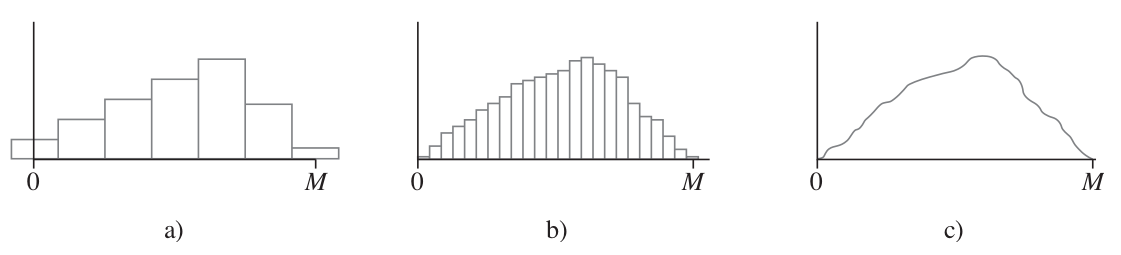
\includegraphics[width=1\linewidth]{material/img/densidad} 

}

\caption{Histogramas de profundidad.}\label{fig:densidad}
\end{figure}

En este sentido, se obtiene la siguiente definición. Sea \(X\) una variable aleatoria continua. Entonces, una \textbf{función de densidad de probabilidad} (fdp) de \(X\) es una función \(f(x)\) tal que para dos números cualesquiera \(a\) y \(b\) con \(a \leq b\),

\[
P(a\leq X\leq b) = \int_a^b f(x)dx
\]
Es decir, la probabilidad de que \(X\) asuma un valor en el intervalo \([a, b]\) es el área sobre este intervalo y bajo la gráfica de la función de densidad, como se ilustra en la figura \ref{fig:densidad2}. La gráfica de \(f(x)\) a menudo se conoce como curva de densidad.

\begin{figure}

{\centering 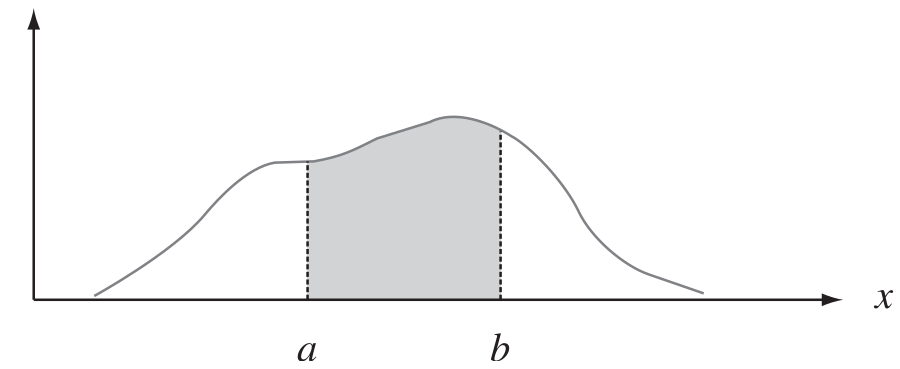
\includegraphics[width=0.7\linewidth]{material/img/densidad2} 

}

\caption{Área debajo de la curva de densidad.}\label{fig:densidad2}
\end{figure}

Al igual que una distribución de masa de probabilidad, se deben cumplir condiciones para que la función de densidad de probabilidad sea legítima. Las condiciones son:

\begin{enumerate}
\def\labelenumi{\arabic{enumi}.}
\tightlist
\item
  \(f(x) \geq 0, \forall x\)
\item
  \(\displaystyle\int_{-\infty}^{\infty} f(x)dx = 1\)
\end{enumerate}

\begin{example}
\protect\hypertarget{exm:intervalotiempo}{}\label{exm:intervalotiempo}

``Intervalo de tiempo'' en el flujo de tránsito es el tiempo transcurrido entre el tiempo en que un carro termina de pasar por un punto fijo y el instante en que el siguiente carro comienza a pasar por ese punto. Sea \(X =\) el intervalo de tiempo de dos carros consecutivos seleccionados al azar en una autopista durante un periodo de tráfico intenso. La siguiente función de densidad de probabilidad de X es en esencia el sugerido en ``The Statistical Properties of Freeway Traffic'' (\emph{Transp. Res}. vol.~11: 221-228):

\[f(x) = 0.15e^{-0.15(x-0.5)} \text{, } x \geq 0.5\]
La gráfica de \(f(x)\) se da en la figura \ref{fig:ejemplo1}; no hay ninguna densidad asociada con intervalos de tiempo de menos de 0.5 y la densidad del intervalo decrece con rapidez (exponencial) a medida que \(x\) se incrementa a partir de 0.5. Claramente, \(f(x) \geq 0\); para demostrar que la integral en todo el dominio de la función es igual a 1, se utiliza el siguiente resultado.

\[
\int_a^{\infty}e^{-kx}dx = \frac{1}{k}e^{-ka}
\]

Entonces,

\begin{equation}
\notag
\begin{split}
\int_{-\infty}^{\infty} f(x)dx &= \int_{0.5}^{\infty} 0.15e^{-0.15(x-0.5)}dx = 0.15e^{0.075}\int_{0.5}^{\infty} e^{-0.15x}dx\\
&= 0.15e^{0.075}\frac{1}{0.15}e^{-0.075} = 1
\end{split}
\end{equation}

\begin{figure}

{\centering 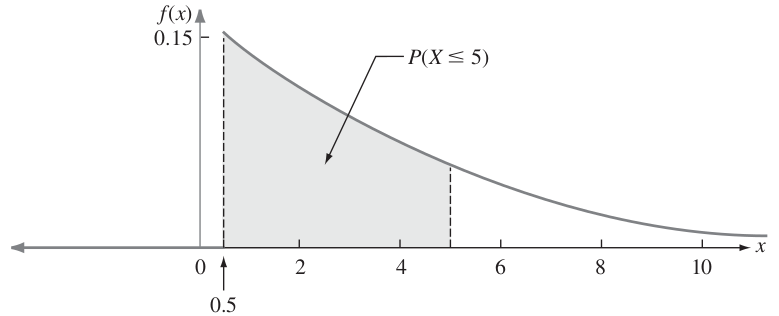
\includegraphics[width=0.7\linewidth]{material/img/ejemplo1} 

}

\caption{Curva de densidad del intervalo de tiempo del ejemplo 2.17.}\label{fig:ejemplo1}
\end{figure}

En R, la gráfica de está función de densidad puede replicarse de la siguiente manera.

\begin{Shaded}
\begin{Highlighting}[]
\NormalTok{fdp }\OtherTok{=} \ControlFlowTok{function}\NormalTok{(x)\{}
\NormalTok{  f }\OtherTok{=} \FloatTok{0.15}\SpecialCharTok{*}\FunctionTok{exp}\NormalTok{(}\SpecialCharTok{{-}}\FloatTok{0.15}\SpecialCharTok{*}\NormalTok{(x}\FloatTok{{-}0.5}\NormalTok{)) }\CommentTok{\# Expresión de la función de densidad}
  \FunctionTok{return}\NormalTok{(f)}
\NormalTok{\}}

\NormalTok{x }\OtherTok{=} \FunctionTok{seq}\NormalTok{(}\FloatTok{0.5}\NormalTok{, }\DecValTok{10}\NormalTok{, }\AttributeTok{by =} \FloatTok{0.01}\NormalTok{) }\CommentTok{\# Valores del dominio}
\NormalTok{f }\OtherTok{=} \FunctionTok{fdp}\NormalTok{(x) }\CommentTok{\# Valores del recorrido}
\NormalTok{df }\OtherTok{=} \FunctionTok{data.frame}\NormalTok{(}\StringTok{"x"} \OtherTok{=}\NormalTok{ x, }\StringTok{"f"} \OtherTok{=}\NormalTok{ f) }\CommentTok{\# Data frame para poder usar ggplot}

\FunctionTok{ggplot}\NormalTok{(}\AttributeTok{data =}\NormalTok{ df, }\FunctionTok{aes}\NormalTok{(}\AttributeTok{x =}\NormalTok{ x, }\AttributeTok{y =}\NormalTok{ f)) }\SpecialCharTok{+} \FunctionTok{geom\_line}\NormalTok{() }\SpecialCharTok{+} 
  \FunctionTok{labs}\NormalTok{(}\AttributeTok{title =} \StringTok{"Función de densidad"}\NormalTok{, }\AttributeTok{x =} \StringTok{"Valores de X"}\NormalTok{, }\AttributeTok{y =} \StringTok{"f(x)"}\NormalTok{)}
\end{Highlighting}
\end{Shaded}

\begin{center}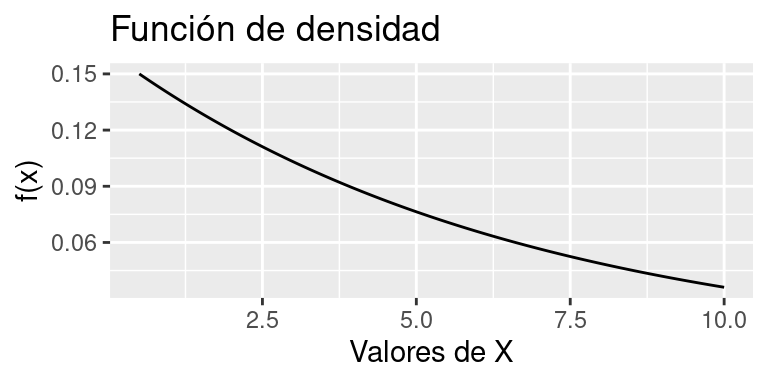
\includegraphics{estadisticas_files/figure-latex/unnamed-chunk-55-1} \end{center}

Así, la probabilidad de que el intervalo de tiempo sea cuando mucho de 5 segundos es

\begin{equation}
\notag
\begin{split}
P(X\leq 5) &= \int_{-\infty}^{5} f(x)dx = \int_{0.5}^{5} 0.15e^{-0.15(x-0.5)}dx\\
&= 0.15e^{0.075}\int_{0.5}^{5} e^{-0.15x}dx = \left. 0.15e^{0.075}\frac{-1}{0.15}e^{-0.15x}\right|_{x = 0.5}^{x = 5}\\
&= e^{0.075}\left(e^{-0.75} + e^{-0.075} \right) = 1.078(-0.472 + 0.928) = 0.491\\
\end{split}
\end{equation}

En R para hacer el cálculo de la integral es posible utilizar el comando \textbf{integrate}:

\begin{Shaded}
\begin{Highlighting}[]
\CommentTok{\# Haciendo uso de la función utilizada para el gráfico}
\FunctionTok{integrate}\NormalTok{(fdp, }\AttributeTok{lower =} \FloatTok{0.5}\NormalTok{, }\AttributeTok{upper =} \DecValTok{5}\NormalTok{)}
\end{Highlighting}
\end{Shaded}

\begin{verbatim}
## 0.4908436 with absolute error < 5.4e-15
\end{verbatim}

\end{example}

\begin{exercise}

Sea \(X\) la cantidad de tiempo durante la cual un libro puesto en reserva durante dos horas en la biblioteca de una universidad es solicitado en préstamo por un estudiante seleccionado y suponga que \(X\) tiene la función de densidad

\[f(x) = 0.5x \text{, } 0\leq x \leq 2\]
Calcule las siguientes probabilidades (manualmente y en R):

\begin{enumerate}
\def\labelenumi{\alph{enumi}.}
\item
  \(P(X \leq 1)\).
\item
  \(P(0.5 \leq X \leq 1.5)\).
\item
  \(P(1.5 < X)\).
\end{enumerate}

\end{exercise}

\begin{exercise}

El error implicado al hacer una medición geográfica computarizada es una variable aleatoria continua \(X\) con función de densidad de probabilidad

\[f(x) = 0.09375(4-x^2) \text{, } -2\leq x \leq 2\]

\begin{enumerate}
\def\labelenumi{\alph{enumi}.}
\item
  Bosqueje la gráfica de \(f(x)\).
\item
  Calcule \(P(X > 0)\).
\item
  Calcule \(P(-1 < X < 1)\).
\item
  Calcule \(P(X < 0.5 \text{ o } X > 0.5)\).
\end{enumerate}

\end{exercise}

\begin{exercise}

Un profesor universitario nunca termina su disertación antes del final de la hora y siempre termina dentro de 2 minutos después de la hora. Sea \(X =\) el tiempo que transcurre entre el final de la hora y el final de la disertación y suponga que la función de densidad de probabilidad de \(X\) es

\[f(x) = kx^2 \text{, } 0\leq x \leq 2\]

\begin{enumerate}
\def\labelenumi{\alph{enumi}.}
\item
  Determine el valor de \(k\) y trace en R la curva de densidad correspondiente.
\item
  ¿Cuál es la probabilidad de que la disertación termine dentro de un minuto del final de la hora?
\item
  ¿Cuál es la probabilidad de que la disertación continúe después de la hora durante entre 60 y 90 segundos.
\item
  ¿Cuál es la probabilidad de que la disertación continúe durante por lo menos 90 segundos después del final de la hora?
\end{enumerate}

\end{exercise}

\subsection{Función de distribución acumulada}\label{funciuxf3n-de-distribuciuxf3n-acumulada-1}

La función de distribución acumulada \(F(x)\) de una variable aleatoria discreta \(X\) da, con cualquier número especificado \(x\), la probabilidad \(P(X \leq x)\). Se obtiene sumando la función masa de probabilidad \(p(y)\) a lo largo de todos los valores posibles y que satisfacen \(y \leq x\). La función de distribución acumulada de una variable aleatoria continua da las mismas probabilidades \(P(X \leq x)\) y se obtiene integrando la función de densidad de probabilidad \(f(y)\) entre los límites \(-\infty\) y \(x\).

La función de distribución acumulada \(F(x)\) de una variable aleatoria continua \(X\) se define para todo número \(x\) como

\[
F(x) =P(X\leq x) = \int_{-\infty}^xf(y)dy
\]

Con cada \(x\), \(F(x)\) es el área bajo la curva de densidad a la izquierda de \(x\). Esto se ilustra en la figura \ref{fig:acumulada}, donde \(F(x)\) se incrementa con regularidad a medida que \(x\) se incrementa.

\begin{figure}

{\centering 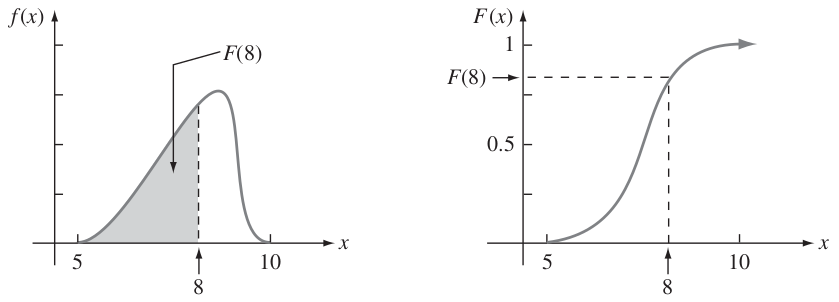
\includegraphics[width=0.7\linewidth]{material/img/acumulada} 

}

\caption{Función de densidad de probabilidad y distribución acumulada asociada}\label{fig:acumulada}
\end{figure}

\begin{example}
\protect\hypertarget{exm:densidad1}{}\label{exm:densidad1}

Suponga que la función de densidad de probabilidad de la magnitud \(X\) de una carga dinámica sobre un puente (en newtons) está dada por

\begin{equation}
  \notag
  f(x) = \left\lbrace
  \begin{matrix}
    \displaystyle\frac{1}{8} + \displaystyle\frac{3}{8}x & 0\leq x \leq 2 \\
    0 & \text{en otro caso}
  \end{matrix} \right.
\end{equation}

Para cualquier número \(x\) entre 0 y 2,

\begin{equation}
  \notag
  F(x) = \int_{-\infty}^xf(y)dy = \int_{0}^x \left(\frac{1}{8} + \frac{3}{8}y\right) dy = \frac{x}{8} + \frac{3}{16}x^2
\end{equation}

Por lo tanto

\begin{equation}
  \notag
  F(x) = \left\lbrace
  \begin{matrix}
    0 & x<0 \\
    \displaystyle\frac{x}{8} + \displaystyle\frac{3}{16}x^2 & 0\leq x \leq 2 \\
    1 & x > 2\\
  \end{matrix} \right.
\end{equation}

\end{example}

La importancia de la función de distribución acumulada en este caso, lo mismo que para variables aleatorias discretas, es que las probabilidades de varios intervalos pueden ser calculadas con una fórmula o una tabla de \(F(x)\). En el caso de una variable aleatoria continua \(X\) con función de densidad de probabilidad \(f(x)\) y función de distribución acumulada \(F(x)\), se tiene que con cualquier número \(a\),

\[
P(X>a) = 1 - F(a)
\]

y para dos números cualesquiera \(a\) y \(b\) con \(a<b\).

\[
P(a\leq X \leq b) = F(b) - F(a)
\]
La figura \ref{fig:densidad3} ilustra la probabilidad deseada es el área sombreada bajo la curva de densidad entre \(a\) y \(b\), que es igual a la diferencia entre las dos áreas sombreadas acumulativas. Esto es diferente de lo que es apropiado para una variable aleatoria discreta de valor entero.

\begin{figure}

{\centering 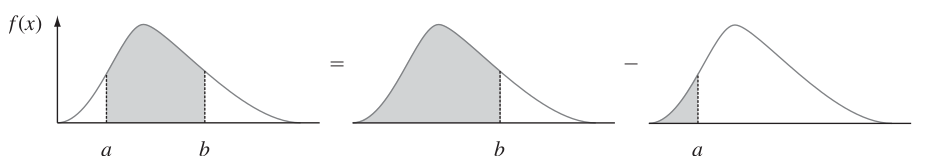
\includegraphics[width=0.8\linewidth]{material/img/densidad3} 

}

\caption{Cálculo de probabilidades acumulativas.}\label{fig:densidad3}
\end{figure}

\begin{example}
Continuando con el ejemplo \ref{exm:densidad1}. Las gráficas de \(f(x)\) y \(F(x)\) son

\begin{Shaded}
\begin{Highlighting}[]
\NormalTok{densidad }\OtherTok{=} \ControlFlowTok{function}\NormalTok{(x)\{ }\CommentTok{\# Función de densidad}
  \FunctionTok{return}\NormalTok{(}\DecValTok{1}\SpecialCharTok{/}\DecValTok{8}\SpecialCharTok{+}\DecValTok{3}\SpecialCharTok{/}\DecValTok{8}\SpecialCharTok{*}\NormalTok{x)}
\NormalTok{\}}
\NormalTok{acumulada }\OtherTok{=} \ControlFlowTok{function}\NormalTok{(x)\{ }\CommentTok{\# Función de distribución acumulada}
  \FunctionTok{return}\NormalTok{(x}\SpecialCharTok{/}\DecValTok{8}\SpecialCharTok{+}\DecValTok{3}\SpecialCharTok{/}\DecValTok{16}\SpecialCharTok{*}\NormalTok{x}\SpecialCharTok{\^{}}\DecValTok{2}\NormalTok{)}
\NormalTok{\}}

\NormalTok{df }\OtherTok{=} \FunctionTok{data.frame}\NormalTok{(}\StringTok{"x"} \OtherTok{=} \FunctionTok{seq}\NormalTok{(}\DecValTok{0}\NormalTok{,}\DecValTok{2}\NormalTok{,}\FloatTok{0.01}\NormalTok{), }\CommentTok{\# Valores de X}
                \StringTok{"fx"} \OtherTok{=} \FunctionTok{densidad}\NormalTok{(}\FunctionTok{seq}\NormalTok{(}\DecValTok{0}\NormalTok{,}\DecValTok{2}\NormalTok{,}\FloatTok{0.01}\NormalTok{)), }\CommentTok{\# Valores de la densidad}
                \StringTok{"Fx"} \OtherTok{=} \FunctionTok{acumulada}\NormalTok{(}\FunctionTok{seq}\NormalTok{(}\DecValTok{0}\NormalTok{,}\DecValTok{2}\NormalTok{,}\FloatTok{0.01}\NormalTok{))) }\CommentTok{\# Valores acumulados}

\CommentTok{\# Gráfico de línes de ambas funciones}
\FunctionTok{ggplot}\NormalTok{(}\AttributeTok{data =}\NormalTok{ df) }\SpecialCharTok{+}
  \FunctionTok{geom\_line}\NormalTok{(}\FunctionTok{aes}\NormalTok{(}\AttributeTok{x =}\NormalTok{ x, }\AttributeTok{y =}\NormalTok{ fx, }\AttributeTok{color =} \StringTok{"Densidad"}\NormalTok{)) }\SpecialCharTok{+}
  \FunctionTok{geom\_line}\NormalTok{(}\FunctionTok{aes}\NormalTok{(}\AttributeTok{x =}\NormalTok{ x, }\AttributeTok{y =}\NormalTok{ Fx, }\AttributeTok{color =} \StringTok{"Acumulada"}\NormalTok{)) }\SpecialCharTok{+}
  \FunctionTok{labs}\NormalTok{(}\AttributeTok{color =} \StringTok{"Función"}\NormalTok{, }\AttributeTok{x =} \StringTok{"Valores de X"}\NormalTok{, }\AttributeTok{y =} \StringTok{""}\NormalTok{)}
\end{Highlighting}
\end{Shaded}

\begin{center}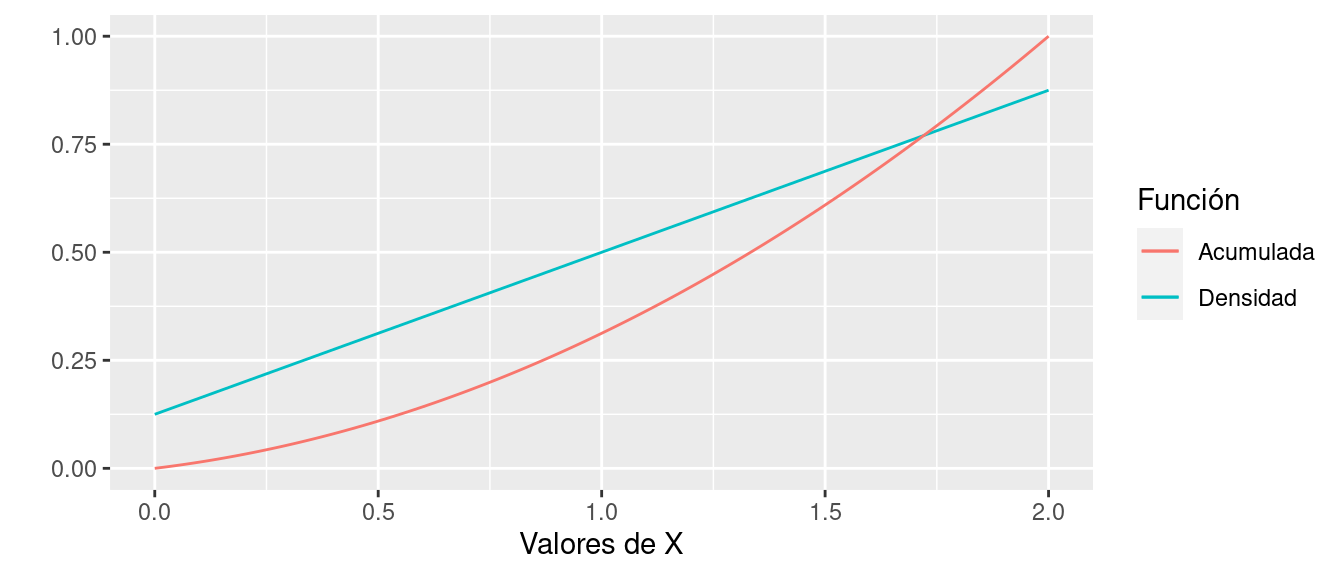
\includegraphics{estadisticas_files/figure-latex/unnamed-chunk-57-1} \end{center}

La probabilidad de que la carga esté entre 1 y 1.5 es

\[P(1 \leq X \leq 1.5) = F(1.5) - F(1)\]
Utilizando la función del gráfico para la función de distribución acumulada, el resultado es

\begin{Shaded}
\begin{Highlighting}[]
\FunctionTok{acumulada}\NormalTok{(}\FloatTok{1.5}\NormalTok{) }\SpecialCharTok{{-}} \FunctionTok{acumulada}\NormalTok{(}\DecValTok{1}\NormalTok{)}
\end{Highlighting}
\end{Shaded}

\begin{verbatim}
## [1] 0.296875
\end{verbatim}

Una vez que se obtiene la función de distribución acumulada, cualquier probabilidad que implique \(X\) es fácil de calcular sin cualquier integración adicional.
\end{example}

\begin{exercise}

Sea \(X\) la cantidad de tiempo durante la cual un libro puesto en reserva durante dos horas en la biblioteca de una universidad es solicitado en préstamo por un estudiante seleccionado. La función de distribución acumulativa del tiempo de préstamo \(X\) es

\begin{equation}
  \notag
  F(x) = \left\lbrace
  \begin{matrix}
    0 & x<0 \\
    \displaystyle\frac{x^2}{4} & 0\leq x < 2 \\
    1 & x \geq 2\\
  \end{matrix} \right.
\end{equation}

Use esta para calcular lo siguiente:

\begin{enumerate}
\def\labelenumi{\alph{enumi}.}
\tightlist
\item
  \(P(X \leq 1)\)
\item
  \(P(0.5 \leq X \leq 1)\)
\item
  \(P(X > 0.5)\)
\item
  \(f(x)\)
\item
  Grafique \(f(x)\) y \(F(x)\).
\end{enumerate}

\end{exercise}

\begin{exercise}

El error de medición de un proceso de control de gestión en la peligrosidad de residuos está dado por la siguiente función de distribución acumulada.

\begin{equation}
  \notag
  F(x) = \left\lbrace
  \begin{matrix}
    0 & x < -2 \\
    \displaystyle\frac{1}{2} + \displaystyle\frac{3}{32}\left(4x-\displaystyle\frac{x^3}{3}\right) & -2\leq x < 2 \\
    1 & x \geq 2\\
  \end{matrix} \right.
\end{equation}

\begin{enumerate}
\def\labelenumi{\alph{enumi}.}
\tightlist
\item
  Calcule \(P(X < 0)\).
\item
  Calcule \(P(-1 < X < 1)\).
\item
  Calcule \(P(0.5 < X)\).
\item
  Calcule \(f(x)\).
\item
  Grafique \(f(x)\) y \(F(x)\).
\end{enumerate}

\end{exercise}

\begin{exercise}

El ejemplo \ref{exm:intervalotiempo} introdujo el concepto de intervalo de tiempo en el flujo de tránsito y propuso una distribución particular para \(X =\) el intervalo de tiempo entre dos carros consecutivos seleccionados al azar (s). Suponga que en un entorno de tránsito diferente, la distribución del intervalo de tiempo tiene la forma

\begin{equation}
  \notag
  f(x) = \left\lbrace
  \begin{matrix}
    \displaystyle\frac{k}{x^4} & x > 1 \\
    0 & x \leq 1\\
  \end{matrix} \right.
\end{equation}

\begin{enumerate}
\def\labelenumi{\alph{enumi}.}
\tightlist
\item
  Determine el valor de \(k\) con el cual \(f(x)\) es una función de densidad de probabilidad legítima.
\item
  Obtenga la función de distribución acumulada.
\item
  Use la función de distribución acumulada de \((b)\) para determinar la probabilidad de que el intervalo de tiempo exceda de 2 segundos y también la probabilidad de que el intervalo esté entre 2 y 3 segundos.
\item
  Grafique la función de densidad de probabilidad y la función de distribución acumulada.
\end{enumerate}

\end{exercise}

\subsection{Distribuciones}\label{distribuciones-1}

A continuación, se dan a conocer algunas de las distribución de probabilidad continua más utilizadas. Cabe mencionar, que existen muchas otras distribuciones, por lo que se invita al estudiante a informarse de ellas en caso de que lo requiera.

\subsubsection{Uniforme}\label{uniforme-1}

Esta es una versión continua de la ya vista en modelos discretos, la diferencia radica en que la variable es del tipo continua valga la redundancia. La función de probabilidad asociada es:

\begin{equation}
\notag
f(x) = \left\lbrace
\begin{array}{cl}
\displaystyle\frac{1}{b-a} & \text{si } x \in (a,b)\\
0 & \text{si } x \not\in (a,b)
\end{array}
\right.
\end{equation}

\textbf{Notación}: \(U(a,b)\)

\begin{example}
Imagine que es un analista financiero encargado de analizar los rendimientos diarios de una acción en particular en el mercado de valores. Los rendimientos diarios de esta acción se distribuyen de manera uniforme continua entre \(-2\%\) y \(2\%\), es decir, \(U(a = -2, b = 2)\).

En este caso, la distribución uniforme continua significa que cada valor dentro del rango dado tiene la misma probabilidad de ocurrir. Por lo tanto, la probabilidad de que el rendimiento diario de la acción sea cualquier valor entre \(-2\%\) y \(2\%\) es igual.

Supongamos que estás interesado en calcular la probabilidad de que el rendimiento diario de la acción sea mayor o igual a \(1.2\%\). Para hacerlo, primero debemos calcular el ancho del rango en el cual el rendimiento se encuentra dentro o por encima del \(1.2\%\). En este caso, el ancho del rango es \(2\% - 1.2\% = 0.8\%\).

La probabilidad de que el rendimiento diario sea mayor o igual a \(1.2\%\) es igual al ancho del rango (\(0.8\%\)) dividido por el ancho total de la distribución (\(4\%\) en este caso), lo cual resulta en \(0.8\%/4\% = 0.2\).
\end{example}

La figura \ref{fig:simuniformecontinua}, muestra una simulación de la función de densidad de probabilidad de la distribución uniforme continua.

\begin{figure}

{\centering 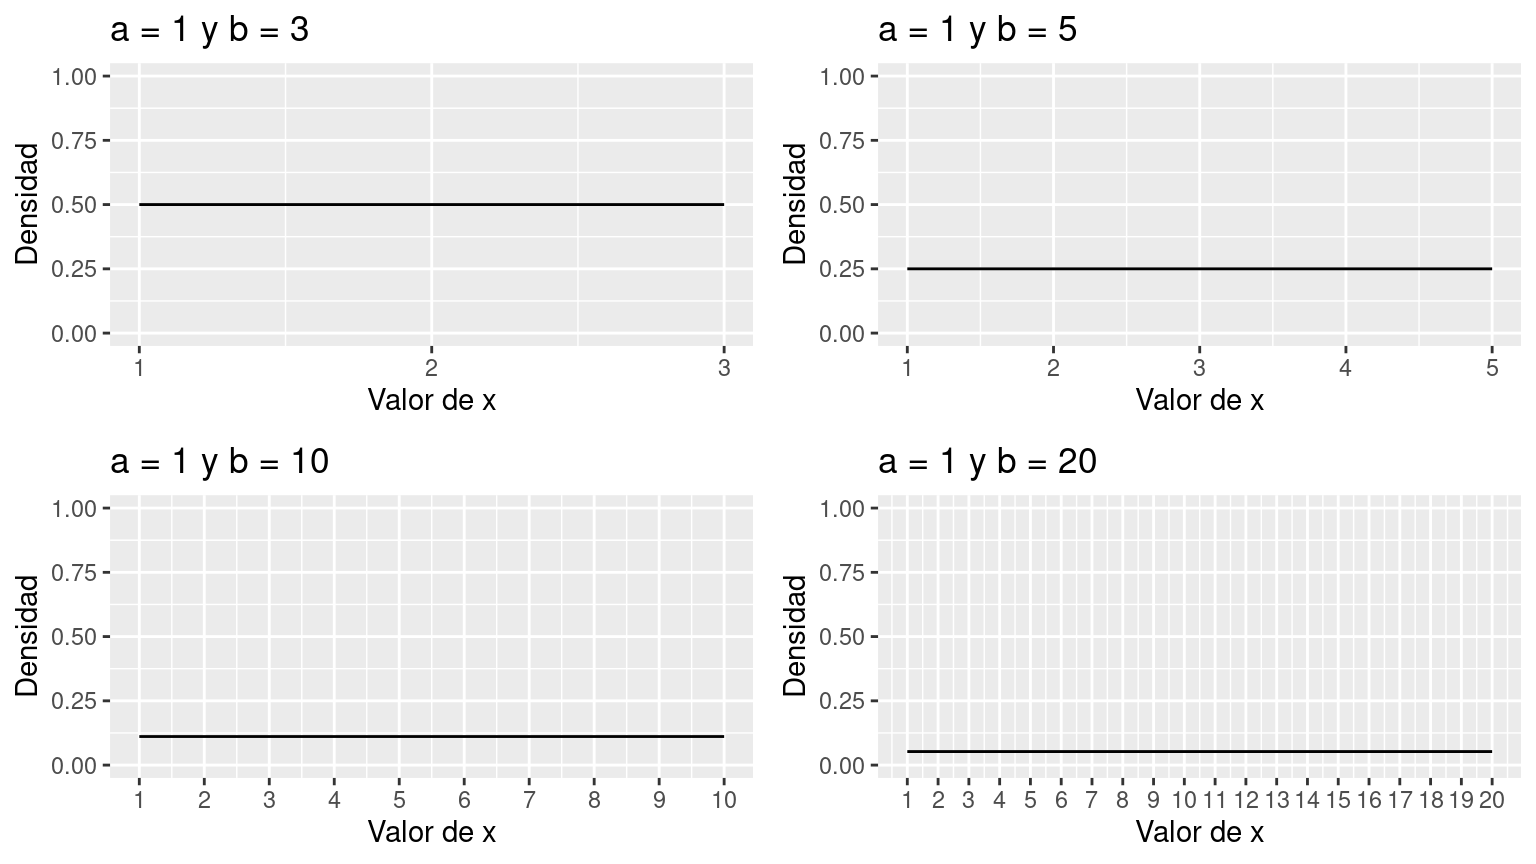
\includegraphics{estadisticas_files/figure-latex/simuniformecontinua-1} 

}

\caption{Simulación de la distribución Uniforme Continua}\label{fig:simuniformecontinua}
\end{figure}

\subsubsection{Exponencial}\label{exponencial}

Esta es una de las pocas variables aleatorias continuas que se aplica a un contexto de determinado. Se utiliza para modelar tiempos de espera para la ocurrencia de un determinado evento (éxito). \textbf{¿Qué similitudes y diferencias tiene con la variable discreta Poisson?}.

La función de densidad asociada es:

\begin{equation}
\notag
f(x)= \left\lbrace
\begin{array}{cl}
\lambda e^{ -\lambda x} & \text{si } x \geq 0\\
0 & \text{si } x < 0
\end{array}
\right.
\end{equation}

con \(\lambda > 0\). ¿Qué interpretación tiene lambda?

\textbf{Notación}: \(\text{Exp}(\lambda)\)

La figura \ref{fig:simexponencial}, muestra una simulación de la función de densidad de probabilidad de la distribución exponencial.

\begin{figure}

{\centering 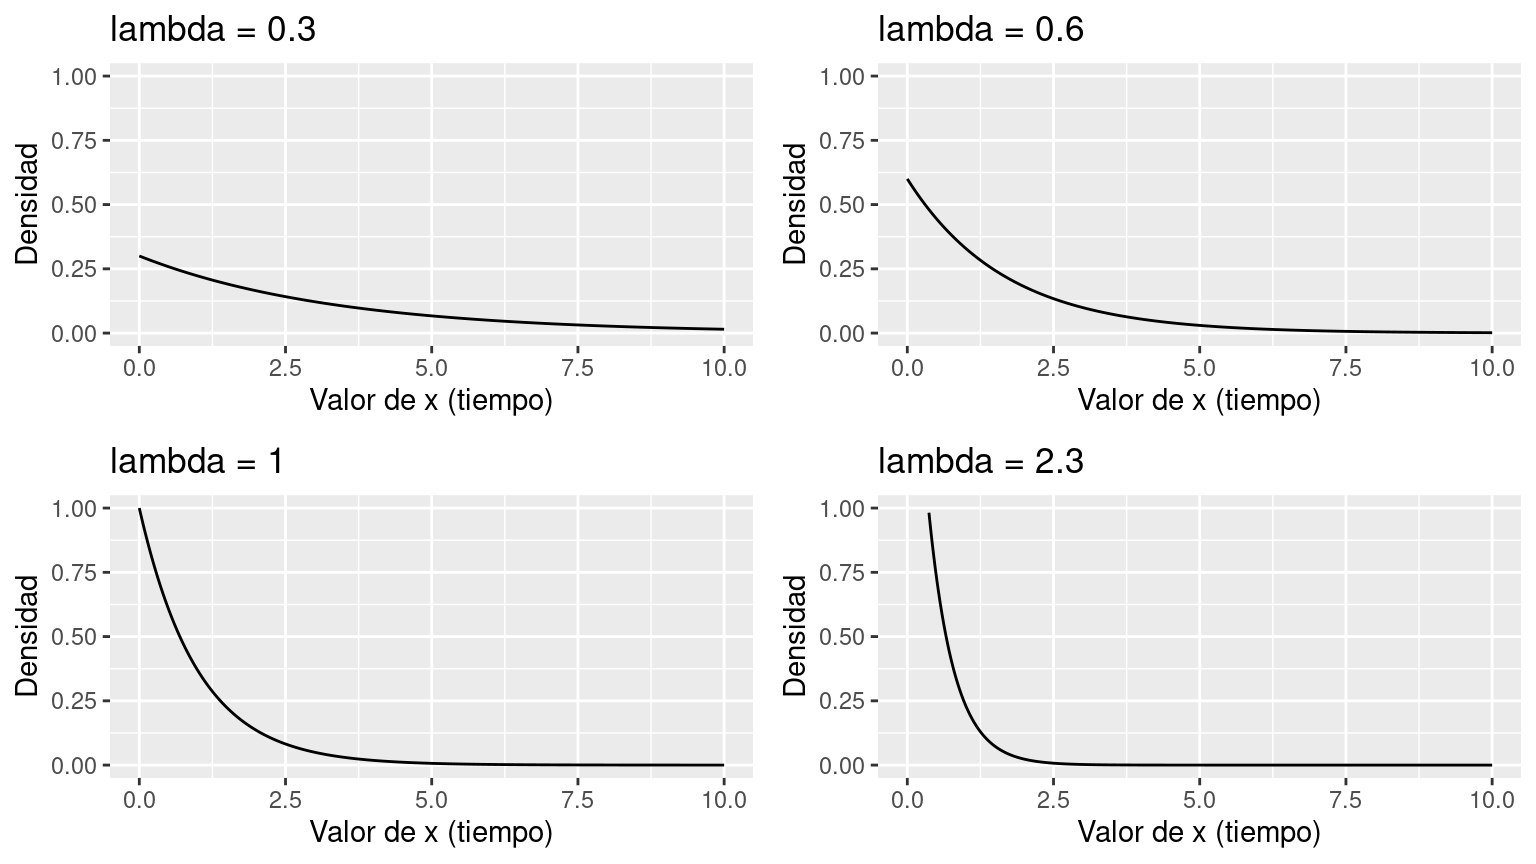
\includegraphics{estadisticas_files/figure-latex/simexponencial-1} 

}

\caption{Simulación de la distribución Exponencial}\label{fig:simexponencial}
\end{figure}

\begin{example}

Se está analizando el tiempo de espera de los clientes en una tienda y se desea calcular la probabilidad de que un cliente tenga que esperar más de 15 minutos antes de ser atendido. Suponiendo que el tiempo promedio de espera es de 10 minutos, es posible utilizar la distribución exponencial para calcular esta probabilidad.

Lambda se calcula como el el recíproco del tiempo promedio, es decir, \(\lambda = \frac{1}{10}\). Luego, se desea calcular

\[
P(X > 15)
\]

En R:

\begin{Shaded}
\begin{Highlighting}[]
\FunctionTok{pexp}\NormalTok{(}\DecValTok{15}\NormalTok{,}
     \AttributeTok{rate =} \DecValTok{1}\SpecialCharTok{/}\DecValTok{10}\NormalTok{, }\CommentTok{\# Lambda}
     \AttributeTok{lower.tail =}\NormalTok{ F)}
\end{Highlighting}
\end{Shaded}

\begin{verbatim}
## [1] 0.2231302
\end{verbatim}

\end{example}

En la tabla \ref{tab:continuaRexponencial} se muestran los comandos para calcular probabilidades asociadas a esta distribución.

\begin{table}[H]
\centering
\caption{\label{tab:continuaRexponencial}Cálculo de probabilidades de la distribución exponencial en R.}
\centering
\begin{tabular}[t]{>{\raggedright\arraybackslash}p{3cm}>{\raggedright\arraybackslash}p{8cm}}
\toprule
Probabilidad & Comando\\
\midrule
$P(X \leq x)$ o $P(X \lt x)$ & pexp(q = , rate = )\\
$P(X \geq x)$ o $P(X \gt x)$ & pexp(q = , rate = , lower.tail = F)\\
$P(X \leq q) = p$ & qexp(p = , rate = )\\
\bottomrule
\end{tabular}
\end{table}

\begin{exercise}
Un componente eléctrico tiene una vida útil media de 8 años. Si su vida útil se distribuye en forma exponencial. ¿Cuál debe ser el tiempo \(x\) de garantía que se debe otorgar, si se desea reemplazar a lo más el \(15\%\) de los componentes que fallen dentro de este período?
\end{exercise}

\begin{exercise}
Las personas que solicitan créditos en un banco son sometidas a un estudio de morosidad. En general, el tiempo promedio de una persona para volverse morosa es de 4 años después de solicitar un crédito. Si el momento en que una persona se vuelve morosa distribuye de forma exponencial con \(x\) en años, ¿cuál es la probabilidad de que una persona se vuelva morosa posterior al quinto año después de solicitar un crédito?
\end{exercise}

\begin{exercise}
Las rutas de reparto de pedidos de Amazon en Chile son modificadas en promedio cada año. Si el tiempo de actualización de las rutas distribuye de forma exponencial con \(x\) en años, ¿cuál es la probabilidad de que las rutas de reparto se actualicen al cabo de 13 meses?
\end{exercise}

\subsubsection{Normal}\label{normal}

Esta es una de la variables continuas más usadas. Lamentablemente, no existe un característica fenomenológica que permita deducir cuando es adecuado utilizar esta variable. La función de desindad de probabilidad asociada es la siguiente.

\begin{equation}
\notag
f(x)= (2\pi \sigma^2)^{-1/2}e^{\left( -\displaystyle\frac{(x-\mu)^2}{2\sigma^2} \right)} ,x \in R
\end{equation}

\textbf{Notación}: \(N(\mu, \sigma^2)\)

La figura \ref{fig:simnormal}, muestra una simulación de la función de densidad de probabilidad de la distribución normal.

\begin{figure}

{\centering 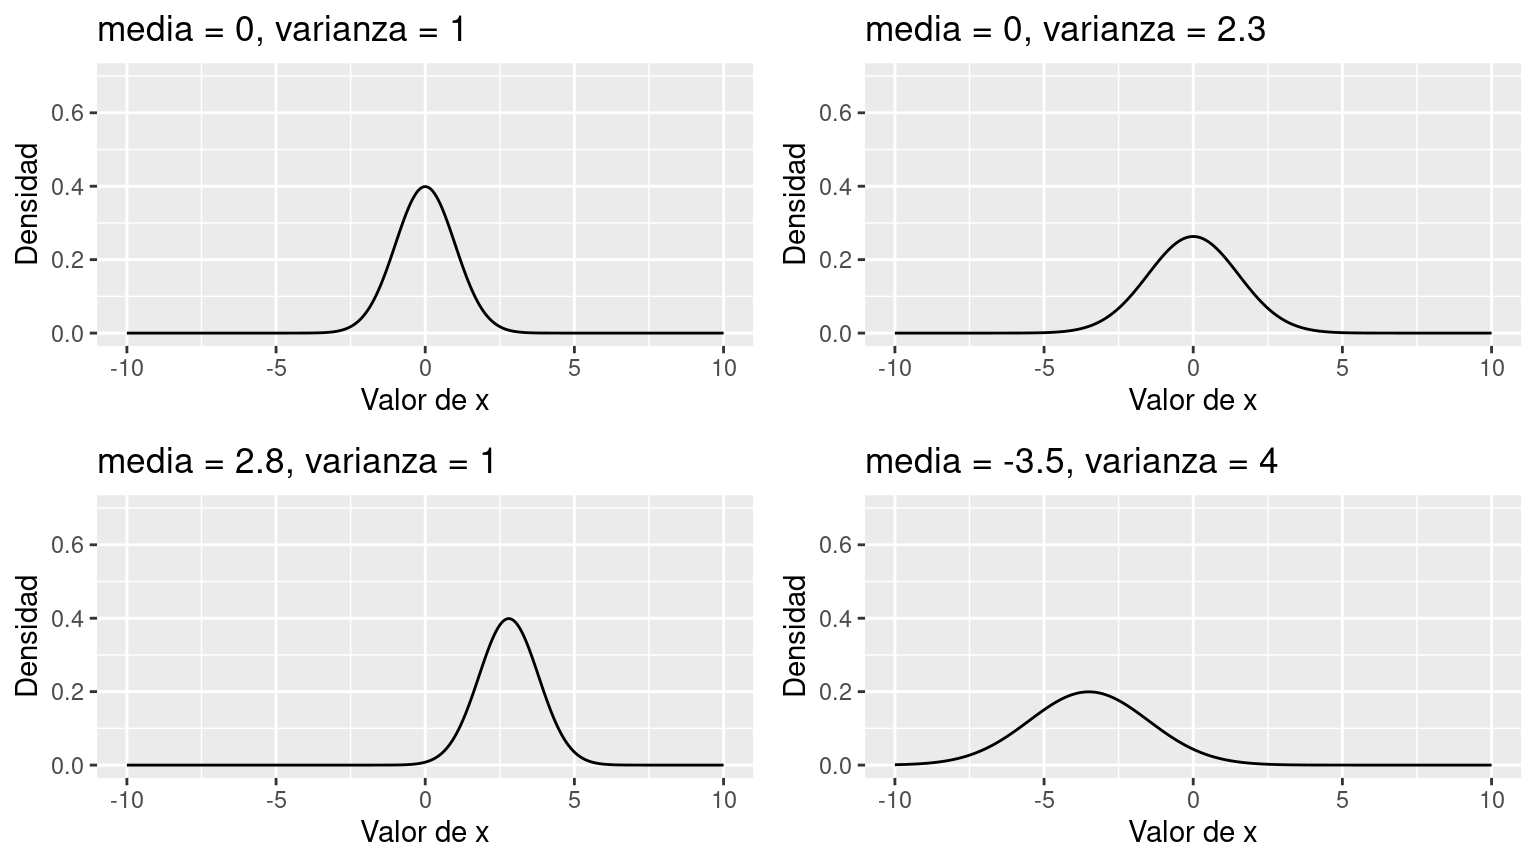
\includegraphics{estadisticas_files/figure-latex/simnormal-1} 

}

\caption{Simulación de la distribución Normal}\label{fig:simnormal}
\end{figure}

\begin{example}

Se está analizando los ingresos mensuales de una empresa y se desea calcular la probabilidad de que los ingresos estén por debajo de \(\$6000\) miles de dólares. Además, se sabe que los ingresos mensuales siguen una distribución normal con una media de \(\$5000\) (miles de dólares )y una desviación estándar de \(\$1000\) (miles de dólares).

La probabilidad a calcular es \(P(X < 6000)\). En R:

\begin{Shaded}
\begin{Highlighting}[]
\FunctionTok{pnorm}\NormalTok{(}\AttributeTok{q =} \DecValTok{6000}\NormalTok{, }\AttributeTok{mean =} \DecValTok{5000}\NormalTok{, }\AttributeTok{sd =} \DecValTok{1000}\NormalTok{)}
\end{Highlighting}
\end{Shaded}

\begin{verbatim}
## [1] 0.8413447
\end{verbatim}

\end{example}

En la tabla \ref{tab:continuaRnormal} se muestran los comandos para calcular probabilidades asociadas a esta distribución.

\begin{table}[H]
\centering
\caption{\label{tab:continuaRnormal}Cálculo de probabilidades de la distribución normal en R.}
\centering
\begin{tabular}[t]{>{\raggedright\arraybackslash}p{3cm}>{\raggedright\arraybackslash}p{8cm}}
\toprule
Probabilidad & Comando\\
\midrule
$P(X \leq x)$ o $P(X \lt x)$ & pnorm(q = , mean = , sd = )\\
$P(X \geq x)$ o $P(X \gt x)$ & pnorm(q = , mean = , sd = , lower.tail = F)\\
$P(X \leq q) = p$ & qnorm(p = , mean = , sd = )\\
\bottomrule
\end{tabular}
\end{table}

\begin{exercise}
En un bar se ha instalado una máquina automática para la venta de cerveza. La máquina puede regularse de modo que la cantidad media de cerveza por vaso sea la que se desea. Además, se sabe que el proceso de llenado sigue una distribución normal, y que independiente de la cantidad a llenar la desviación estándar es 5.9 \(ml\). Si el nivel medio se ajusta a 304.6 \(ml\) determine qué porcentaje de los vasos contendrá menos de 295.7 \(ml\).
\end{exercise}

\begin{exercise}
Cada cierto periodo de tiempo, el Banco Central de Chile realiza una inyección de capital al mercado chileno, con el fin de mermar el efecto de la inflación. El dinero que destina el banco, sigue un distribución normal con media 15 (miles de millones) y una varianza de 4 (miles de millones). ¿Cuál es probabilidad el banco inyecte más de 15.6 miles de millones de pesos?
\end{exercise}

\begin{exercise}

La mayoría de las transacciones electrónicas en Chile están a cargo de la empresa Transbank. Además, se sabe que la cantidad de transacciones realizadas por Transbank sigue un distribución normal con una media de 20 millones.

\begin{itemize}
\item
  Si la varianza de las transacciones es de 25 millones, ¿cuál es la probabilidad de que Transbank esté a cargo de más de 30 millones de transacciones?
\item
  Si la varianza de las transacciones es de 16 millones, ¿cuántas deben ser las transacciones para que la probabilidad de que Transbank se haga cargo de un número mayor sea de un 34\%?
\end{itemize}

\end{exercise}

\begin{exercise}

El tipo de cambio del euro ha fluctuado de manera similar al dólar en los últimos 4 años. Si valor observado del euro sigue un distribución normal con media \$912 y varianza \$144.

\begin{itemize}
\item
  ¿Cuál es la probabilidad de que el tipo de cambio del euro supere los \$920?
\item
  ¿A cuánto debe estar el tipo de cambio para que la probabilidad de que el euro supere ese valor sea de un 21.9\%?
\end{itemize}

\end{exercise}

\begin{exercise}

Los residuos de vuelo de una determinad aerolínea son recolectados al final de cada semana, generando en promedio 48 toneladas de residuos. Además, la cantidad de residuos generados por los vuelos sigue una distribución normal.

\begin{itemize}
\item
  Si la varianza de los residuos generados es de 100, ¿cuál es la probabilidad de que la aerolínea genere más de 50 toneladas de residuos?
\item
  Si la varianza de los residuos generados es de 120, ¿cuántos deben ser los residuos para que la probabilidad de que la aerolínea genere menos sea de un 87\%?
\end{itemize}

\end{exercise}

\begin{exercise}

El sistema logístico de lavado de autos de una determinada empresa ha optado por instalar una máquina automática para la atención de clientes. Se sabe que la cantidad de clientes que son atendidos por la máquina sigue una distribución normal con una varianza de 90 personas.

\begin{itemize}
\item
  Si el promedio de personas atendidas por la máquina es de 390, ¿cuál es la probabilidad de que la máquina atienda a menos de 385 personas?
\item
  Si el promedio de personas atendidas por la máquina son de 360, ¿cuántas personas como mínimo que deben ir a la máquina para que la posibilidad de que sean atendidas sea de un 70\%?
\end{itemize}

\end{exercise}

\subsubsection{T - Student y Ji - Cuadrado}\label{t---student-y-ji---cuadrado}

Estas dos variables, al igual que la Normal son muy utilizadas. Sin embargo, la función de densidad de cada una de ellas es más compleja y engorrosa.

Los parámetros de cada una de ellas son lo siguientes:

\begin{itemize}
\tightlist
\item
  \emph{t} - Student: \(t(v)\), donde \(v\) son los denominados grados de libertad.
\item
  \(\chi^2\): \(\chi^2(v)\), donde \(v\) son los denominados grados de libertad.
\end{itemize}

La distribución \emph{t} - Student y la Normal son muy parecidas cuando el tamaño de la muestra es grande. Además, en R se tiene que, la distribución \emph{t} - Student siempre tiene media 0 y varianza fija \(> 1\) (una especie de parámetros fijos).

La figura \ref{fig:simstudent}, muestra una simulación de la función de densidad de probabilidad de la distribución \emph{t} - Student

\begin{figure}

{\centering 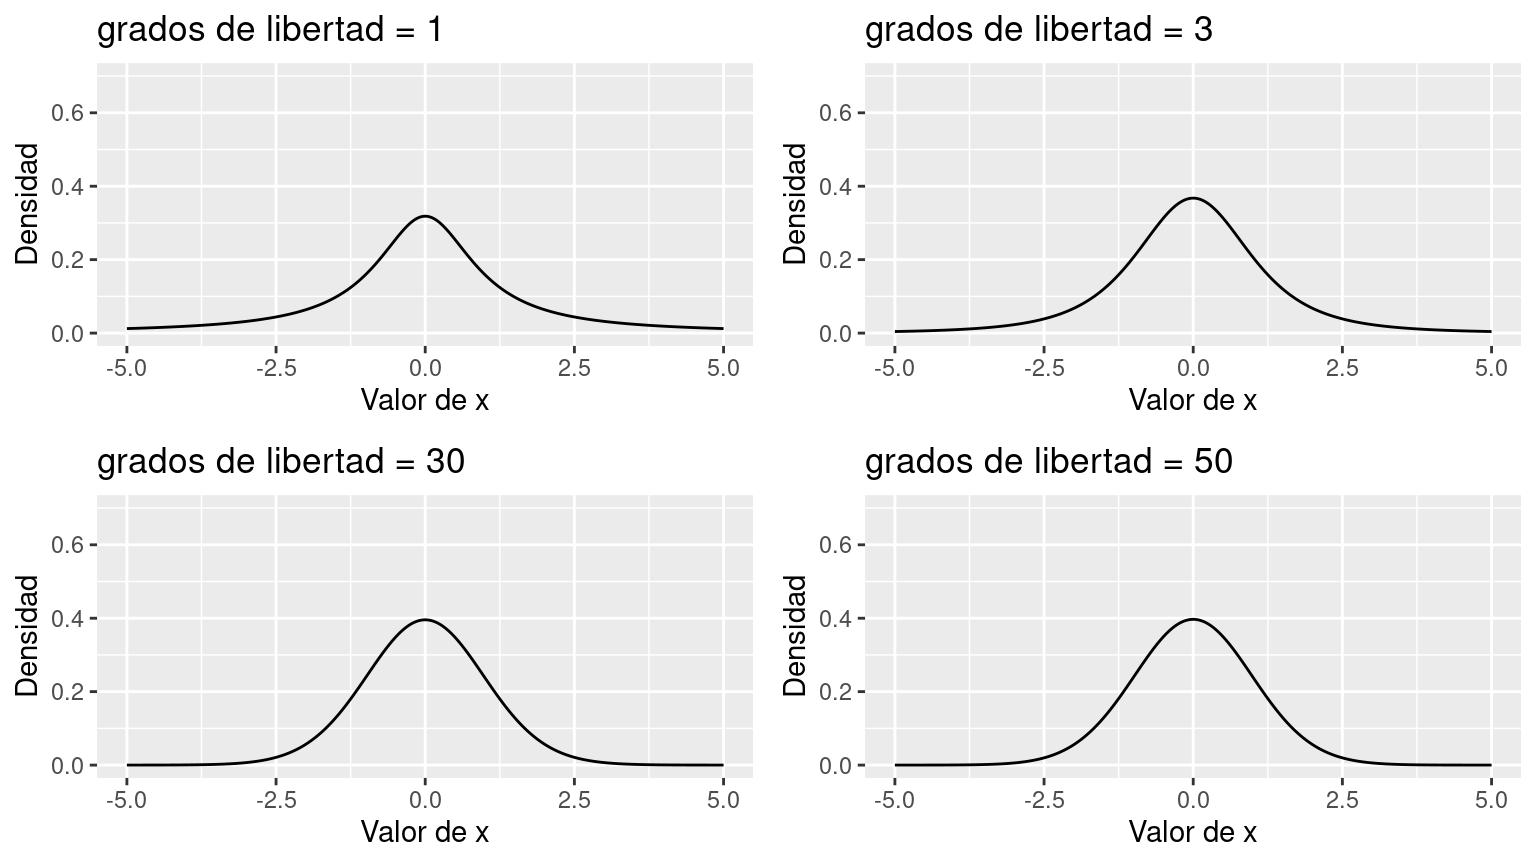
\includegraphics{estadisticas_files/figure-latex/simstudent-1} 

}

\caption{Simulación de la distribución t-Student}\label{fig:simstudent}
\end{figure}

La figura \ref{fig:simchi}, muestra una simulación de la función de densidad de probabilidad de la distribución Ji-Cuadrado

\begin{figure}

{\centering 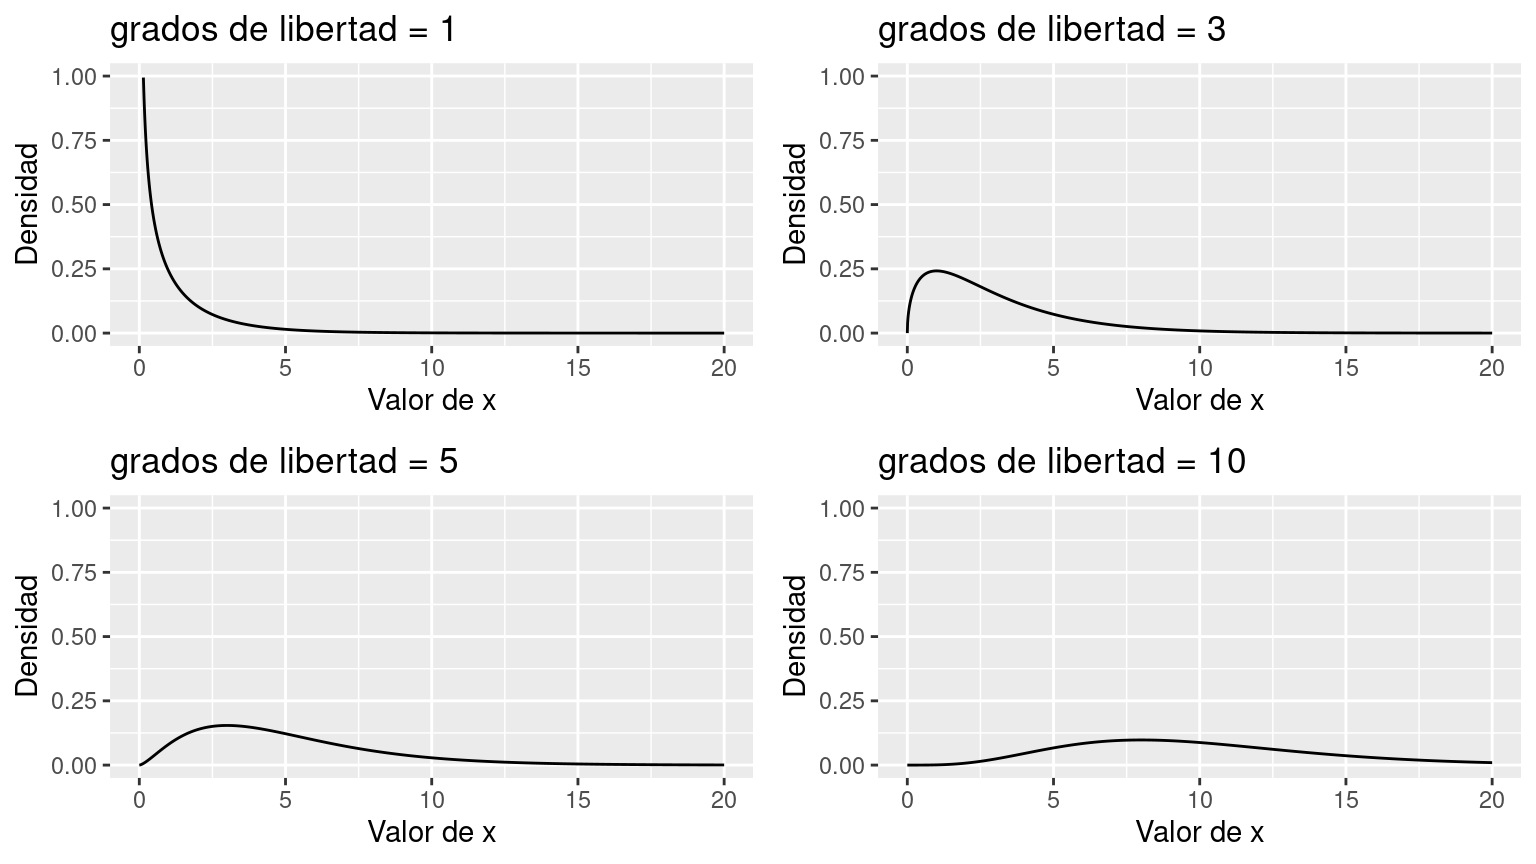
\includegraphics{estadisticas_files/figure-latex/simchi-1} 

}

\caption{Simulación de la distribución Ji-Cuadrado}\label{fig:simchi}
\end{figure}

En la tabla \ref{tab:continuaRtchisq} se muestran los comandos para calcular probabilidades asociadas a estas distribuciones.

\begin{table}[H]
\centering
\caption{\label{tab:continuaRtchisq}Cálculo de probabilidades de la distribución t-student y Ji-Cuadrado en R.}
\centering
\begin{tabular}[t]{>{\raggedright\arraybackslash}p{3cm}>{\raggedright\arraybackslash}p{4cm}>{\raggedright\arraybackslash}p{4cm}}
\toprule
Probabilidad & T-Student & Ji-Cuadrado\\
\midrule
$P(X \leq x)$ o $P(X \lt x)$ & pt(q = , df = ) & pchisq(q = , df = )\\
$P(X \geq x)$ o $P(X \gt x)$ & pt(q = , df = , lower.tail = F) & pchisq(q = , df = , lower.tail = F)\\
$P(X \leq q) = p$ & qt(p = , df = ) & qchisq(p = , df = )\\
\bottomrule
\end{tabular}
\end{table}

\begin{exercise}
Durante los últimos años, la cantidad de de personas que han solicitado avances en efectivo en cajeros automáticos ha ido en aumento. Si la cantidad de solicitudes de avances (en miles) siguen un distribución \(\chi^2\) con 34 grados de libertad, ¿cuál es probabilidad de que para este año la cantidad de avances realizados en cajero sea menor a 45 mil?
\end{exercise}

\begin{exercise}
La cantidad de fraudes financieros han ido en aumento a medida que la tecnología avanza. Si la cantidad de fraudes (en miles) sigue una distribución \emph{t} - Student con 51 grados de libertad, ¿cuál es probabilidad de que para este año la cantidad de fraudes sea mayor a 0.7 mil?
\end{exercise}

\begin{exercise}
La empresa ROSEN tiene un sistema automático para el relleno de almohadas con plumas. Si el volumen de relleno de plumas de las almohadas sigue un distribución \emph{t} - Student con 200 grados de libertad, ¿cuál es la probabilidad de que una almohada sea rellenada con menos de 0.5 mil plumas?
\end{exercise}

Por otro lado, la tabla \ref{tab:densidadcontinuasR} muestra un resumen de los comandos en R para los distintos casos de cálculo de valores en la función de densidad con distribuciones continuas.

\begin{table}[H]
\centering
\caption{\label{tab:densidadcontinuasR}Cálculo de densidades de distribuciones continuas en R.}
\centering
\resizebox{\ifdim\width>\linewidth\linewidth\else\width\fi}{!}{
\begin{tabular}[t]{>{\raggedright\arraybackslash}p{3cm}>{\raggedright\arraybackslash}p{3cm}>{\raggedright\arraybackslash}p{3cm}>{\raggedright\arraybackslash}p{3cm}l}
\toprule
Densidad & Normal & Exponencial & T-Student & Ji-Cuadrado\\
\midrule
$f(x)$ & dnorm(x = , mean = , sd = ) & dexp(x = , rate =) & dt(x = , df =) & dchisq(x = , df =)\\
\bottomrule
\end{tabular}}
\end{table}

\section{Esperanza}\label{esperanza}

La esperanza, esperanza matemática o valor medio, es un concepto que se aplica cuando un experimento es realizado muchas veces. Consideremos un dado honesto, es decir, la probabilidad de que cada una de las caras salga seleccionada en cada tiro es de 1/6. Si registramos cada uno de los resultados y luego los promediamos, ese resultado es el resultado final promedio. Sin embargo, nosotros podemos estar interesados en conocer ese valor sin la necesidad de tener que tirar el dado muchas veces, para ello, existen fórmulas que permiten calcular el valor promedio de los resultados al realizar el experimento muchas veces.

Si se trabaja con una variable aleatoria discreta, la esperanza matemática está dada por la siguiente expresión

\begin{equation}
\notag
\mu = E(X) = \sum_{i=1}^n x_iP(X = x_i)
\end{equation}
\label{eq:esperanzadiscreta}

Por otro lado, para una variable aleatoria continua la expresión es

\begin{equation}
\notag
\mu = E(X) = \int_{-\infty}^{\infty} xf(x)dx
\label{eq:esperanazacontinua}
\end{equation}

\begin{example}
Consideremos el lanzamiento del dado, del cual se habló anteriormente. La siguiente tabla, refleja la probabilidad de cada uno de los eventos

\begin{table}[H]
\centering
\begin{tabular}[t]{lc}
\toprule
$X$ & $P(X = x_i)$\\
\midrule
1 & 1/6\\
2 & 1/6\\
3 & 1/6\\
4 & 1/6\\
5 & 1/6\\
6 & 1/6\\
\bottomrule
\end{tabular}
\end{table}

Haciendo uso de la fórmula de esperanza agregamos los valores de la expresión \(x_if(x_i)\).

\begin{table}[H]
\centering
\begin{tabular}[t]{lcc}
\toprule
$X$ & $P(X = x_i)$ & $x_iP(X=x_i)$\\
\midrule
1 & 1/6 & 1/6\\
2 & 1/6 & 2/6\\
3 & 1/6 & 3/6\\
4 & 1/6 & 4/6\\
5 & 1/6 & 5/6\\
6 & 1/6 & 1\\
\bottomrule
\end{tabular}
\end{table}

Finalmente, se deben sumar los valores de la tercera columna, obteniéndose como resultado

\begin{equation}
\notag
E(X) = \sum_{i=1}^n x_iP(X=x_i) = 1/6 + 2/6 +3/6 + 4/6 + 5/6 + 6/6 = 21/6 = 3.5
\end{equation}

En base a este resultado, si una persona cobra 3 mil pesos por cada lanzamiento del dado, y devuelve 4 mil cada vez que el jugador obtiene un numero mayor a 2, ¿es rentable jugar?, ¿por qué?
\end{example}

\begin{example}

Sea \(X\) una variable aleatoria con distribución

\begin{equation}
\notag
P(X=x) = p(1-p)^{x-1}, x = 1,2,\ldots
\end{equation}

Determine \(E(X)\).

\begin{equation}
\notag
\begin{split}
E(X) &= \sum_{i=1}^{\infty}x_iP(X=x_i) = \sum_{x=1}^{\infty}xP(X=x)  = \sum_{x=1}^{\infty}xp(1-p)^{x-1}\\ 
&= p\sum_{x=1}^{\infty}x(1-p)^{x-1}  = p\sum_{x=1}^{\infty}\frac{\partial}{\partial p}\left(-(1-p)^{x}\right)\\ 
&= -p\frac{\partial}{\partial p}\left(\sum_{x=1}^{\infty}(1-p)^{x}\right)  = -p\frac{\partial}{\partial p}\left(\sum_{x=0}^{\infty}(1-p)^{x}-1\right)\\ 
&= -p\frac{\partial}{\partial p}\left(\frac{1}{1-(1-p)}-1\right) =  -p\frac{\partial}{\partial p}\left(\frac{1-p}{p}\right)\\ 
&= -p\frac{-p - (1-p)}{p^2} = \frac{1}{p}
\end{split}
\end{equation}

\end{example}

Si \(X\) es una variable aleatoria y \(a,b\) y \(c\) son valores reales constantes, entonces, se tiene las siguientes propiedades de la espranza:

\begin{enumerate}
\def\labelenumi{\arabic{enumi}.}
\tightlist
\item
  \(E(k) = k\) si \(k\) es una constante.
\item
  \(E(kX) = kE(X)\).
\item
  \(E(aX+b) = aE(X) + b\).
\item
  Sea \(X\) una v.a.d, entonces, \(E(h(X)) = \displaystyle\sum_{i=1}^n h(x_i)P(X = x_i)\).
\item
  Sea \(X\) una v.a.c, entonces, \(E(h(X)) = \displaystyle\int_{-\infty}^{\infty} h(x)f(x)dx\).
\end{enumerate}

\begin{exercise}
Un juego de azar consiste en lanzar dos dados y ganar tantos miles de pesos como valga la suma de las puntuaciones de los dados. ¿Cual es la cantidad media ganada cada vez que juego? Si me cobran 5 mil pesos por cada juego, ¿es interesante participar en este juego?
\end{exercise}

\begin{exercise}
\protect\hypertarget{exr:exesperanza1}{}\label{exr:exesperanza1}Para una variable aleatoria discreta \(X\) la distribución de probabilidad viene dada por

\begin{equation}
\notag
P(X = x) = \left\lbrace 
\begin{matrix}
kx & x = 1,2,3,4,5\\
k(10-x) & x = 6,7,8,9
\end{matrix}
\right.
\end{equation}

Hallar el valor de la constante \(k\) y \(E(X)\).
\end{exercise}

\begin{exercise}
(Verificación con R) Considere la variable aleatoria que representa el número que pudiese salir en una ruleta (del 1 al 36). Determine el valor medio del experimento asociado a jugar en la ruleta. Verifique su resultado generando 10, 20, 30, 100, 200, 500, 1000, 2000 y 5000 números aleatorios enteros (entre 1 y 36, inclusive ambos) en R, realice un gráfico de puntos con líneas entre la cantidad de números aleatorios generados y el promedio de ellos. Comente lo observado.
\end{exercise}

\begin{exercise}
\protect\hypertarget{exr:exesperanza2}{}\label{exr:exesperanza2}

Un distribuidor de enseres para el hogar vende tres modelos de congeladores verticales de 13.5, 15.9 y 19.1 pies cúbicos de espacio de almacenamiento, respectivamente. Sea
\(X =\) la cantidad de espacio de almacenamiento adquirido por el siguiente cliente que compre un congelador. Suponga que \(X\) tiene la función masa de probabilidad

\begin{table}[H]
\centering
\begin{tabular}[t]{cccc}
\toprule
$x$ & 13.5 & 15.9 & 19.2\\
$p(x)$ & 0.2 & 0.5 & 0.3\\
\bottomrule
\end{tabular}
\end{table}

\begin{enumerate}
\def\labelenumi{\arabic{enumi}.}
\tightlist
\item
  Calcule \(E(X)\).
\item
  Calcule \(E(X^2)\).
\end{enumerate}

\end{exercise}

\begin{exercise}
\protect\hypertarget{exr:exesperanza3}{}\label{exr:exesperanza3}

Se selecciona al azar un individuo que tiene asegurado su automóvil con una compañía. Sea \(Y\) el número de infracciones de tránsito por las que el individuo fue citado durante los últimos 3 años. La función masa de probabilidad de \(Y\) es

\begin{table}[H]
\centering
\begin{tabular}[t]{ccccc}
\toprule
$y$ & 0 & 1 & 2 & 3\\
$p(y)$ & 0.6 & 0.25 & 0.1 & 0.05\\
\bottomrule
\end{tabular}
\end{table}

\begin{enumerate}
\def\labelenumi{\arabic{enumi}.}
\tightlist
\item
  Calcule \(E(Y)\).
\item
  Suponga que un individuo con \(Y\) infracciones incurre en un recargo de \(\$100Y^2\). Calcule la cantidad esperada del recargo.
\end{enumerate}

\end{exercise}

\begin{exercise}
\protect\hypertarget{exr:exesperanza4}{}\label{exr:exesperanza4}Una barra de 12 pulgadas que está sujeta por ambos extremos se somete a una cantidad creciente de esfuerzo hasta que se rompe. Sea \(Y =\) la distancia del extremo izquierdo al punto donde ocurre la ruptura. Suponga que \(Y\) tiene la función de densidad de probabilidad

\begin{equation}
\notag
f(y) = \left\lbrace
\begin{matrix}
\displaystyle\frac{y}{24}\left( 1 -\displaystyle\frac{y}{12}  \right) & 0\leq y \leq 12\\
0 & \text{en otro caso}
\end{matrix}
\right.
\end{equation}

Calcule \(E(Y)\) y \(E(Y^2)\).
\end{exercise}

\begin{exercise}
\protect\hypertarget{exr:exesperanza5}{}\label{exr:exesperanza5}El tiempo \(X\) para la terminación de cierta tarea tiene una función de distribución acumulativa \(F(x)\) dada por

\begin{equation}
\notag
F(x) = \left\lbrace
\begin{matrix}
0 & x < 0\\
\displaystyle\frac{x^3}{3} & 0 \leq x < 1\\
1-\displaystyle\frac{1}{2}\left(\displaystyle\frac{7}{3}-x \right)\left(\displaystyle\frac{7}{4}-\displaystyle\frac{3x}{4}\right) & 1\leq x \leq \displaystyle\frac{7}{3}\\
1 & x \geq \displaystyle\frac{7}{3}
\end{matrix}
\right.
\end{equation}

Calcule \(E(X)\) y \(E(X^2)\).
\end{exercise}

\section{Varianza}\label{varianza}

Al igual como se abordó en la unidad 1, la varianza mide la dispersión cuadrática de una variable respecto al promedio. Sin embargo la expresión que permite calcular la varianza de cualquier tipo de variable aleatoria es

\begin{equation}
\sigma^2 = Var(X) = E[(X-\mu)^2]
\label{eq:varianzaVA}
\end{equation}

Utilizando las propiedades de la esperanza, es posible reducir la expresión \eqref{eq:varianzaVA} a una más sencilla.

\begin{equation}
\begin{split}
\sigma^2 = Var(X) &= E[(X-\mu)^2]\\
&= E[X^2-2X\mu + \mu^2]\\
&= E[X^2]-E[2X\mu] + E[\mu^2]\\
&= E[X^2]-2\mu E[X] + \mu^2\\
&= E[X^2]-2\mu \cdot \mu + \mu^2\\
&= E[X^2]-2\mu^2 + \mu^2\\
&= E[X^2]-(E[X])^2\\
\sigma^2 = Var(X) &= E[X^2]-(E[X])^2\\
\end{split}
\label{eq:varianzaSimplificada}
\end{equation}

\begin{example}
Suponga que se tiene una variable aleatoria continua \(X\) con función de densidad de probabilidad \(f(x)\) dada por:

\begin{equation}
\notag
f(x) = 2x \text{, } 0 \leq x \leq 1 \\
\end{equation}

La media de \(X\), se calcula como:

\[\mu = \int_{0}^{1} x \cdot f(x) \, dx = \int_{0}^{1} 2x^2 \, dx = \left[ \frac{2}{3} x^3 \right] \bigg|_{0}^{1} = \frac{2}{3}\]
La varianza de \(X\) se calcula como:

\[\sigma^2 = \int_{0}^{1} (x - \mu)^2 \cdot f(x) \, dx\]
Sustituyendo \(\mu= 2/3\), la fórmula se simplifica a:

\[\sigma^2 = \int_{0}^{1} \left( x - \frac{2}{3} \right)^2 \cdot 2x \, dx\]
La solución de la integral para obtener la varianza es \(1/18\).
\end{example}

\begin{example}
\protect\hypertarget{exm:falaciadeljugador}{}\label{exm:falaciadeljugador}(\emph{La falacia del jugador}) La siguiente tabla muestra el registro de distintos experimentos asociados a tirar una moneda. En cada uno de ellos, se registra la cantidad de lanzamiento de la moneda, la cantidad de caras, la cantidad de sellos, la diferencia (número de caras - número de sellos) y la proporción (número de caras/número de sellos).

\begin{table}[H]
\centering
\caption{\label{tab:unnamed-chunk-65}Primeros 10 de 1000 instancias de lanzamientos de una moneda.}
\centering
\begin{tabular}[t]{ccccc}
\toprule
Lanzamientos & Caras & Sellos & Diferencia & Proporción\\
\midrule
10 & 5 & 5 & 0 & 1.0000000\\
11 & 4 & 7 & -3 & 0.5714286\\
12 & 6 & 6 & 0 & 1.0000000\\
13 & 5 & 8 & -3 & 0.6250000\\
14 & 8 & 6 & 2 & 1.3333333\\
15 & 4 & 11 & -7 & 0.3636364\\
16 & 10 & 6 & 4 & 1.6666667\\
17 & 8 & 9 & -1 & 0.8888889\\
18 & 8 & 10 & -2 & 0.8000000\\
19 & 7 & 12 & -5 & 0.5833333\\
\bottomrule
\end{tabular}
\end{table}

Fijémonos que ocurre si graficamos las diferencias entre caras y sellos según la cantidad de veces se lanza la moneda.

\begin{center}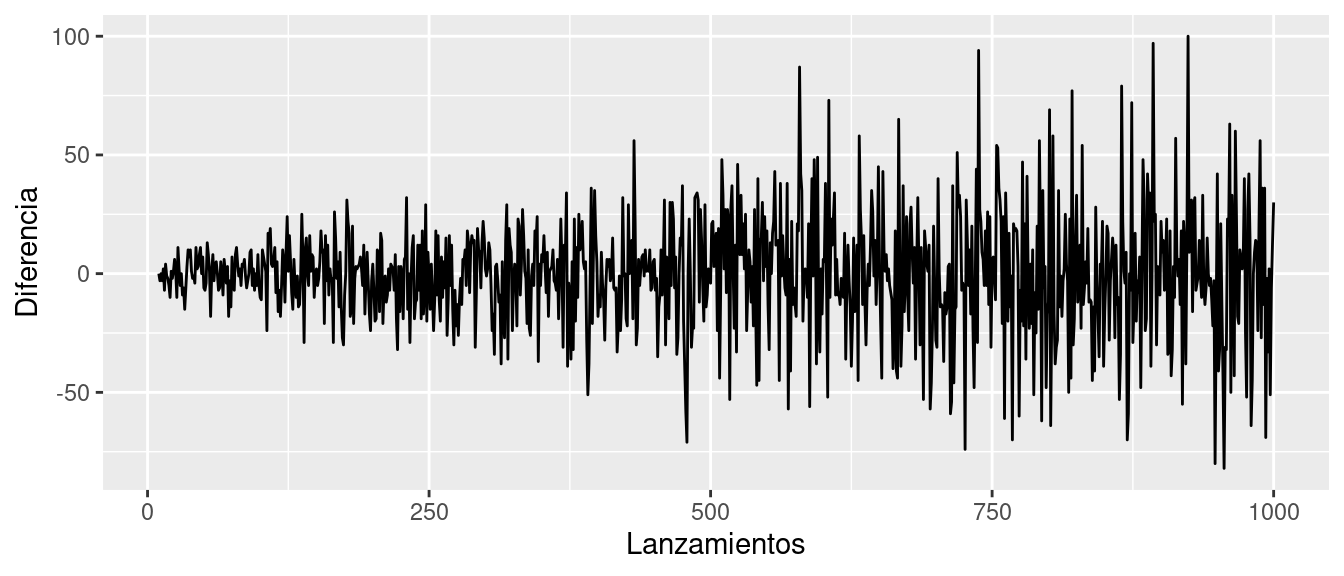
\includegraphics{estadisticas_files/figure-latex/unnamed-chunk-66-1} \end{center}

Por lo que se puede observar, la diferencia (amplitud vertical, variabilidad) aumenta a medida que también lo hace la cantidad de lanzamientos. Este resultado puede parecer extraño, ya que cuantas más veces se lanza la moneda, el números de caras y el de sellos debería tender a acercarse puesto que la cara y el sello son igual de probables. Sin embargo, para apreciar lo que realmente ocurre, se debe graficar las proporciones y no las diferencias.

\begin{center}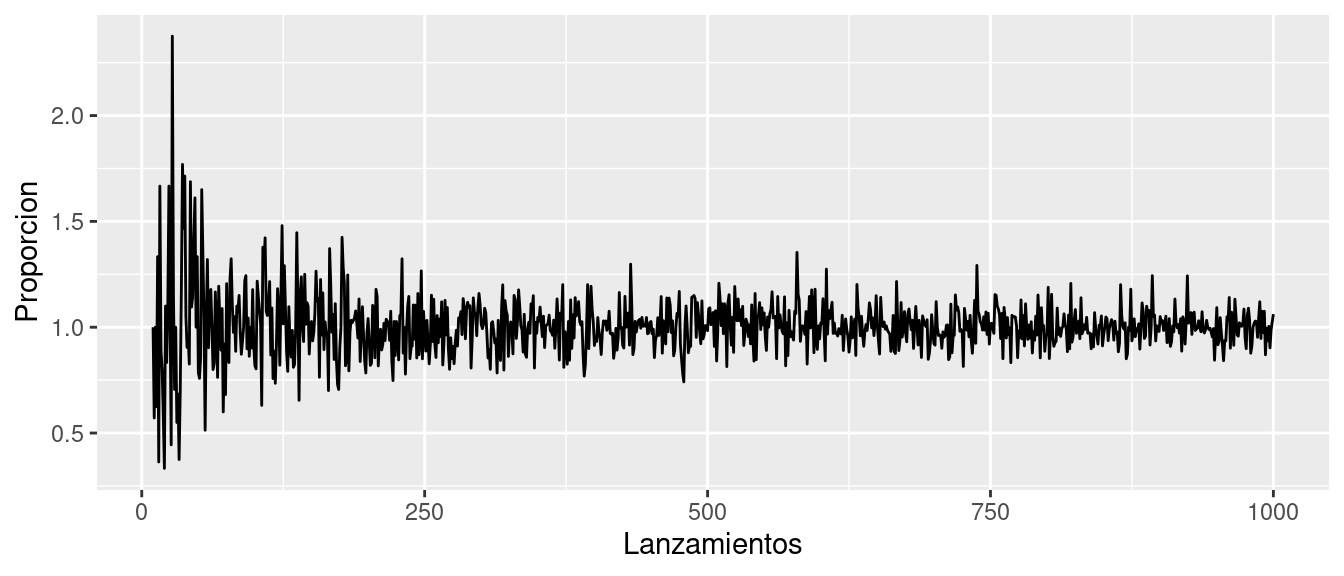
\includegraphics{estadisticas_files/figure-latex/unnamed-chunk-67-1} \end{center}

Como se observa, la proporción de caras y sellos tiene a ser 1 cuántas más veces se arroje la moneda \textbf{(la diferencia también tenderá a cero, pero se necesitan muchos más intentos)}.

La conocida como falacia del jugador consiste en creer que, porque hayan salido de forma continuada un número de caras relativamente grande, en la siguiente jugada deberá salir sello puesto que los resultados deberán compensarse. Así, en una ruleta, si han salido 3 o 4 veces seguidas números de color rojo, pensar que en el siguiente movimiento de la ruleta es más probable que salga negro es una falacia. Cada jugada es independiente de la anterior.

Otros planteamientos (incorrectos) equivalentes son: ``Un resultado aleatorio tiene más probabilidades de ocurrir, si no ha ocurrido durante cierto periodo de tiempo''; o ``Un resultado tiene menos probabilidades de ocurrir, si no ha ocurrido durante cierto periodo de tiempo''.
\end{example}

\begin{exercise}
Calcule la varianza de los siguientes ejercicios \ref{exr:exesperanza1}, \ref{exr:exesperanza2}, \ref{exr:exesperanza3}, \ref{exr:exesperanza4} y \ref{exr:exesperanza5}. Realice el cálculo manualmente y confirme el resultado mediante R.
\end{exercise}

\begin{exercise}

Los ingresos de la empresa TechSolid están definidos por una variable aleatoria \(X\) (en miles de millones de dólares). Se sabe que la la función de densidad de probabilidad está dada por:

\begin{equation}
\notag
f(x) = \frac{1}{4} e^{-x/4},  x \geq 0
\end{equation}

\begin{enumerate}
\def\labelenumi{\arabic{enumi}.}
\tightlist
\item
  Determine el ingreso medio de la empresa.
\item
  Determine la varianza del ingreso de la empresa. Utilice expresamente \(E[(X-\mu)^2]\).
\item
  Si los costos de la empresa se relacionan con los ingresos de la siguiente manera: \(0.02X^2\). Determine los costos promedio de la empresa.
\end{enumerate}

\end{exercise}

\begin{exercise}

Dada la siguiente función de densidad de probabilidad, determine la \(Var(X)\).

\begin{equation}
\notag
f(x) = 4.5 e^{-4.5x} \text{ , } x \geq 0
\end{equation}

\end{exercise}

\chapter{Distribuciones muestrales}\label{distribuciones-muestrales}

Antes de iniciar esta sección es necesario aclarar el concepto de independencia. Para ello, consideremos dos variable aleatorias, y un evento de cada una, podemos entender la independencia como ``la probabilidad de que ocurran los dos eventos al mismo tiempo es igual a la multiplicación de las probabilidades de cada evento por separado''. Además, si las variables (que definen los eventos) tienen la misma función de distribución, se dice que las variables aleatorias son \textbf{independientes idénticamente distribuidas} (iid).

\section{Distribución de muestreo de la media}\label{distribuciuxf3n-de-muestreo-de-la-media}

\subsection{Estandarización}\label{estandarizaciuxf3n}

La estandarización, es un proceso mediante el cual los datos originales de una variable se transforman en una nueva escala que tiene una media de cero y una desviación estándar de uno. Esto permite eliminar las diferencias de escala entre las variables y facilita la comparación y el análisis estadístico \citep{hair2013multivariate}.

Consideremos \(X\) una variable aleatoria normalmente distribuida con media \(E(X) = \mu\) y varianza \(Var(X) = \sigma^2\). El proceso de estandarización de la variable aleatoria es:

\begin{equation}
\frac{X-\mu}{\sigma} \sim N(0,1)
\label{eq:estandarizacion}
\end{equation}

En el gráfico \ref{fig:ejestand} se observa una ejemplificación de la estandarización. Al estandarizar el punto más alto de la curva se centra al rededor del 0, a su vez que la curva se angosta.

\begin{figure}

{\centering 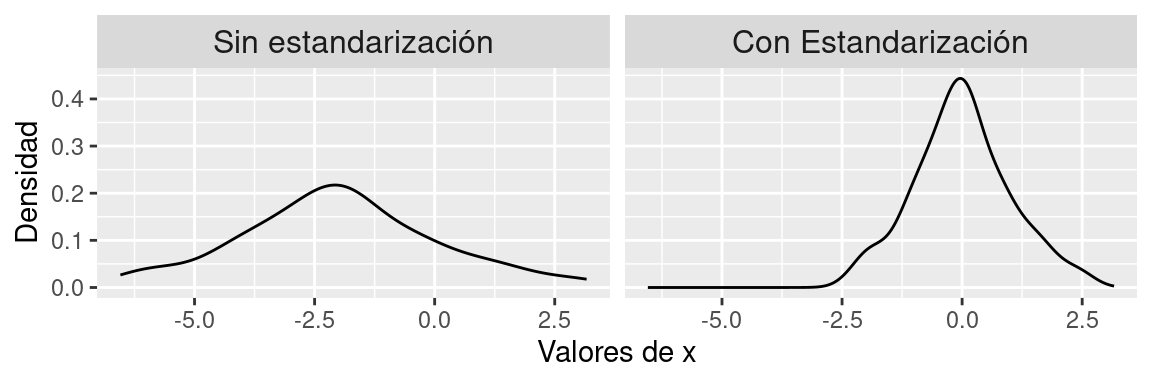
\includegraphics{estadisticas_files/figure-latex/ejestand-1} 

}

\caption{Estandarización de una variable con distribución Normal}\label{fig:ejestand}
\end{figure}

\subsection{Distribución de la media}\label{distribuciuxf3n-de-la-media}

Una de las medidas de resumen más importantes es la media (o promedio) de un conjunto de variables aleatorias independientes e idénticamente distribuidas.

Consideremos \(X_1, \ldots , X_n\) un conjunto de \(n\) variables aleatorias (\emph{iid}), tales que, \(E(X_i) = \mu\) y \(Var(X_i) = \sigma^2\).

Entonces el estadístico

\begin{equation}
\notag
\bar{X} = (X_1 + \cdots + X_n)/n,
\end{equation}

se define como la media de las \(n\) variables aleatorias \emph{iid}

\begin{equation}
\notag
\begin{split}
E(\bar{X}) &= \mu\\
Var(\bar{X}) &= \sigma^2/n
\end{split}
\end{equation}

Una extensión de lo anterior es:

Sea \(X_1, \ldots , X_n\) una conjunto de \(n\) variables aleatorias independientes normalmente distribuidas con medias \(E(X_i) = \mu_i\) y varianzas \(Var(X_i) = \sigma_i^2\) para \(i=1,\ldots,n\). Entonces la distribución de la media muestral es

\begin{equation}
\bar{X}\sim N(\mu,\sigma^2/n)
\label{eq:distMedia}
\end{equation}

Con las propiedades mencionadas, es posible determinar la probabilidad de que ocurran determinados eventos que estén asociados al promedio, siempre y cuando las variables aleatorias tengan una distribución normal.

\begin{example}
\protect\hypertarget{exm:media1}{}\label{exm:media1}El tipo de cambio del dólar a peso chileno cambia diariamente. Supóngase que este valor es una variable aleatoria distribuida normalmente con media \$720 y desviación estándar de \$10.

El gerente de finanzas de una empresa de \emph{retail} a decidido reajustar mensualmente al alza todos los precios de sus productos, cuando el valor promedio del tipo de cambio del dólar sea superior a \$724. Considerando, que se ha tomado una muestra aleatoria de 22 mediciones del dólar del mes anterior, determine la probabilidad de que el gerente aplique un alza en los precios en el próximo mes.

En primer lugar, corresponde plantear la probabilidad que se desea calcular con relación a la aplicación en el alza de precios. En este caso, la variable de estudio tiene distribución normal, por lo cual, la estandarización del promedio de la variable tiene distribución \(N(\mu = 0, \sigma^2=1)\).

\begin{equation}
\notag
\begin{split}
P(\bar{X} > 724) &= P\left(\frac{\bar{X}-\mu}{\sigma/\sqrt{n}} > \frac{724-\mu}{\sigma/\sqrt{n}}\right)\\
&= P\left(\frac{\bar{X}-\mu}{\sigma/\sqrt{n}}  > \frac{724-720}{10/\sqrt{22}}\right)\\
&= P\left(\frac{\bar{X}-\mu}{\sigma/\sqrt{n}}  > 1.876\right)\\
\end{split}
\end{equation}

Luego, el cálculo en R es el siguiente:

\begin{Shaded}
\begin{Highlighting}[]
\FunctionTok{pnorm}\NormalTok{(}\AttributeTok{q =} \FloatTok{1.876}\NormalTok{, }\AttributeTok{mean =} \DecValTok{0}\NormalTok{, }\AttributeTok{sd =} \DecValTok{1}\NormalTok{, }\AttributeTok{lower.tail =}\NormalTok{ F)}
\end{Highlighting}
\end{Shaded}

\begin{verbatim}
## [1] 0.03032764
\end{verbatim}

Finalmente, la probabilidad de que el gerente aplique un alza en los precios en el próximo mes es de 0.03.
\end{example}

\begin{exercise}
La cantidad de operaciones bancarias que ocurren durante un día distribuye normal con media 75 (millones) y varianza 144 (millones). Considerando una muestra de tamaño 22 (días), ¿cuál es la probabilidad de que la media muestral de la cantidad de transacciones sea menor a 77.3 millones?
\end{exercise}

\begin{exercise}
El tiempo que demoran en hacerse efectivas las transferencias bancarias internacionales, distribuye normal con media 15 (segundos) y desviación estándar de 4 (segundos). Considerando una muestra de tamaño 29, ¿cuál es la probabilidad de que la media muestral de los tiempos de demora de transacción sea menor a 14.1 segundos? Mencione con rigurosidad todos los pasos de su solución.
\end{exercise}

\subsection{Teorema del Límite Central}\label{teorema-del-luxedmite-central}

Considerando el ejemplo \ref{exm:media1}, \textbf{¿qué sucede cuándo la variable aleatoria del experimento no sigue una distribución normal?} Para estos casos se utiliza el Teorema del Límite Central (TLC) \citep[página 215]{Devore}.

\begin{itemize}
\tightlist
\item
  \textbf{Anteriormente:}

  \begin{itemize}
  \tightlist
  \item
    (Condición) Las variables aleatorias del problema deben distribuir normal (\emph{iid}).
  \item
    (Resultado) Al estandarizar el promedio, este se transforma en una variable aleatoria normal con media 0 y varianza 1.
  \end{itemize}
\item
  \textbf{Con TLC:}

  \begin{itemize}
  \tightlist
  \item
    Se desconoce si las variable aleatorias del problema distribuyen normal (\emph{iid}).
  \item
    (Condición) La cantidad de datos debe ser grande. Por regla general se utiliza un tamaño mayor a 30, sin embargo, no hay investigaciones o fuentes que lo confirmen \citep{johnson1994sample}.
  \item
    (Resultado) Al estandarizar el promedio, este se transforma en una variable aleatoria normal con media 0 y varianza 1.
  \end{itemize}
\end{itemize}

\begin{example}
Un accionista piensa comprar acciones de una determinada empresa chilena de tecnología. Dado los valores del mercado, se observa que el valor promedio de las acciones (iid) es de \$4000 con una desviación estándar de \$700. El accionista comprará acciones solo si una muestra aleatoria de 100 valores de acciones resulta en un valor promedio mayor a \$4100. ¿Cuál es la probabilidad de que el accionista invierta en la empresa chilena?

Si bien no se especifica que los valores de la acciones distribuyen normal, es posible usar el TLC para determinar la probabilidad.

El planteamiento de la probabilidad es el siguiente:

\begin{equation}
\notag
\begin{split}
P(\bar{X} > 4100) &= P\left(\frac{\bar{X}-\mu}{\sigma/\sqrt{n}} > \frac{4100-\mu}{\sigma/\sqrt{n}}\right)\\
&= P\left(\frac{\bar{X}-\mu}{\sigma/\sqrt{n}} > \frac{4100 - 4000}{700/\sqrt{100}}\right)\\
&= P\left(\frac{\bar{X}-\mu}{\sigma/\sqrt{n}} > 1.428\right)\\
\end{split}
\end{equation}

El cálculo en R es el siguiente:

\begin{Shaded}
\begin{Highlighting}[]
\FunctionTok{pnorm}\NormalTok{(}\AttributeTok{q =} \FloatTok{1.428}\NormalTok{, }\AttributeTok{mean =} \DecValTok{0}\NormalTok{, }\AttributeTok{sd =} \DecValTok{1}\NormalTok{, }\AttributeTok{lower.tail =}\NormalTok{ F)}
\end{Highlighting}
\end{Shaded}

\begin{verbatim}
## [1] 0.07664593
\end{verbatim}

La probabilidad de que el accionista invierta en la empresa chilena es de 0.07
\end{example}

\begin{exercise}
La cantidad de operaciones bancarias que ocurren durante un día tienen una media de 75 (millones) y varianza 144 (millones). Considerando una muestra de tamaño 71 (días), y que se desconoce la distribución de los datos, ¿cuál es la probabilidad de que la media muestral de la cantidad de transacciones sea menor a 73.16 millones? Mencione con rigurosidad todos los pasos de su solución.
\end{exercise}

\begin{exercise}
El tiempo que demoran en hacerse efectivas las transferencias bancarias internacionales tienen una media de 15 (segundos) y desviación estándar de 4 (segundos). Considerando una muestra de tamaño 56, y que se desconoce la distribución de los datos, ¿cuál es la probabilidad de que la media muestral de los tiempos de demora de transacción sea menor a 15.8 segundos? Mencione con rigurosidad todos los pasos de su solución.
\end{exercise}

\begin{exercise}
Supóngase que el número de barriles de petróleo crudo que son importados diariamente es una variable aleatoria con una distribución no especificada. Si se observa la cantidad de barriles importados en 64 días, seleccionados en forma aleatoria , y si se sabe que la desviación estándar del número de barriles por día es \(\sigma = 60\), determínese la probabilidad de que la media muestral se encuentre a no más de 700 barriles del verdadero valor de barriles importados.
\end{exercise}

\section{Distribución de muestreo de la varianza}\label{distribuciuxf3n-de-muestreo-de-la-varianza}

Si la media es una de las medidas de localización más usadas, entonces, la varianza sería aquella con más uso dentro de las medidas de escala. Y al igual que la media, también existe una distribución de muestreo asociada a la varianza muestral.

Consideremos la expresión utilizada para calcular la varianza de un conjunto de datos (muestra):

\begin{equation}
\notag
S^2 = \sum_{i=1}^n\frac{(X_i-\mu)^2}{n-1}
\end{equation}

Se obtiene la siguiente propiedad. Sean \(X_1,\ldots,X_n\) una muestra aleatoria de una distribución normal con media \(\mu\) y varianza \(\sigma^2\). Entonces,

\begin{equation}
Y=\sum_{i=1}^n\frac{(X_i-\mu)^2}{\sigma^2} = \frac{(n-1)S^2}{\sigma^2} \sim \chi^2_{n-1}
\label{eq:distVar}
\end{equation}

\begin{example}
Considere una medición del índice de pobreza (porcentual) proporcionada por un instrumento computacional, en donde el interés recae en la variabilidad de la lectura. Supóngase que, con base en la experiencia, la medición es una variable aleatoria normalmente distribuida con media 14.7 y desviación estándar igual a 1.2 unidades. Si se toma una muestra aleatoria procedente del proceso de medición computacional de tamaño 25, ¿cuál es la probabilidad de que el valor de la varianza muestral del índice de pobreza sea mayor a \(1.1\) unidades?

El planteamiento de la probabilidad es el siguiente.

\begin{equation}
\notag
\begin{split}
P(S^2 > 1.1) &= P\left(\frac{(n-1)S^2}{\sigma^2} > \frac{(n-1)\cdot 1.1}{\sigma^2}\right)\\
&= P\left(\frac{(n-1)S^2}{\sigma^2} > \frac{24\cdot 1.1}{1.2^2}\right)\\
&= P\left(\frac{(n-1)S^2}{\sigma^2} > 18.333\right)\\
\end{split}
\end{equation}

Considerando que esta nueva variable tiene distribución \(\chi^2_{n-1} = \chi^2_{25-1} = \chi^2_{24}\), el cálculo en R es el siguiente:

\begin{Shaded}
\begin{Highlighting}[]
\FunctionTok{pchisq}\NormalTok{(}\AttributeTok{q =} \FloatTok{18.333}\NormalTok{, }\AttributeTok{df =} \DecValTok{24}\NormalTok{, }\AttributeTok{lower.tail =}\NormalTok{ F)}
\end{Highlighting}
\end{Shaded}

\begin{verbatim}
## [1] 0.7865623
\end{verbatim}

Finalmente, la probabilidad de que el valor de la varianza muestral del índice de pobreza sea mayor a \(1.1\) unidades cuadradas es de 0.7865.
\end{example}

\begin{exercise}

Se toma una muestra aleatoria de tamaño 67 proveniente de una población normal con desviación estándar \(\sigma =3.05\). Calcular la probabilidad de que la varianza muestral \(s^{2}\) sea como mínimo 8.21? Utilice solo una de las siguiente tablas.

\begin{minipage}{.45\textwidth} \centering \begin{table}[H]
\centering
\caption{\label{tab:unnamed-chunk-71}Distribución Ji-Cuadrado, df = 66}
\centering
\resizebox{\ifdim\width>\linewidth\linewidth\else\width\fi}{!}{
\begin{tabular}[t]{cc}
\toprule
Cuantil & Probabilidad\\
\midrule
55.24886 & 0.1754\\
56.24816 & 0.2016\\
58.24886 & 0.2597\\
58.54886 & 0.2689\\
59.24886 & 0.2910\\
\bottomrule
\end{tabular}}
\end{table} \end{minipage}
      \begin{minipage}{.45\textwidth} \centering \begin{table}[H]
\centering
\caption{\label{tab:unnamed-chunk-72}Distribución Ji-Cuadrado, df = 65}
\centering
\resizebox{\ifdim\width>\linewidth\linewidth\else\width\fi}{!}{
\begin{tabular}[t]{cc}
\toprule
Cuantil & Probabilidad\\
\midrule
55.24886 & 0.1996\\
56.24816 & 0.2279\\
58.24886 & 0.2895\\
58.54886 & 0.2992\\
59.24886 & 0.3223\\
\bottomrule
\end{tabular}}
\end{table} \end{minipage}

\end{exercise}

\section{La distribución T-Student}\label{la-distribuciuxf3n-t-student}

Hasta el momento sabemos que:

\begin{enumerate}
\def\labelenumi{\arabic{enumi}.}
\item
  \(\displaystyle\frac{\bar{X}-\mu}{\sigma/\sqrt{n}}\sim N(0,1)\)
\item
  \(\displaystyle\frac{nS^2}{\sigma^2}\sim \chi^2_{n}\)
\end{enumerate}

Sin embargo, ¿qué sucede, cuándo no conocemos la varianza poblacional en la distribución de la media?

Para poder trabajar sobre la distribución de la media, reemplazamos la varianza poblacional por la muestral, dando origen a un nuevo estadístico:

\begin{equation}
T = \frac{\bar{X}-\mu}{S/\sqrt{n}} \sim t_{n-1},
\label{eq:distMedia2}
\end{equation}

el cual, es un estadístico \emph{t}-Student con \(n-1\) grados de libertad.

\begin{example}
El Departamento de Protección al Medio Ambiente (DPMA) asegura que, para un automóvil compacto en particular, el consumo promedio de gasolina en carretera es de 45 kilómetros por litro. Una organización independiente de consumidores adquiere uno de estos autos y lo somete a prueba con el propósito de verificar la cifra proporcionada por el DPMA. El auto recorrió una distancia de 100 kilómetros en 25 ocasiones. En cada recorrido se anotó el número de litros necesarios para realizar el viaje. Para los 25 ensayos, la desviación estándar tuvo un valor de 2.5 kilómetros por litro. Si se supone que el número de kilómetros que se recorre por litro es una variable aleatoria distribuida normalmente, ¿cuál es la probabilidad de que el promedio de kilómetros recorridos por litro sea menor al 45.2?

A diferencia de los expuesto anteriormente, no se conoce la varianza poblacional de la variable de estudio (los kilómetros por litro que rinde el automóvil), por lo tanto, corresponde utilizar el estadístico \emph{t}-Student, el cual hace uso de la varianza muestral. El planteamiento de la probabilidad es el siguiente:

\begin{equation}
\notag
\begin{split}
P(\bar{X} < 45.2) &= P\left(\frac{\bar{X}-\mu}{S/\sqrt{n}} < \frac{45.2-\mu}{S/\sqrt{n}}\right)\\
&= P\left(\frac{\bar{X}-\mu}{S/\sqrt{n}} < \frac{45.2 - 45}{2.5/\sqrt{25}}\right)\\
&= P\left(\frac{\bar{X}-\mu}{S/\sqrt{n}} < 0.4\right)\\
\end{split}
\end{equation}

Recordando que esta nueva variable distribuye \(t_{n-1}=t_{25-1}=t_{24}\), el cálculo en R es el siguiente:

\begin{Shaded}
\begin{Highlighting}[]
\FunctionTok{pt}\NormalTok{(}\AttributeTok{q =} \FloatTok{0.4}\NormalTok{, }\AttributeTok{df =} \DecValTok{24}\NormalTok{)}
\end{Highlighting}
\end{Shaded}

\begin{verbatim}
## [1] 0.6536528
\end{verbatim}

la probabilidad de que el promedio de kilómetros recorridos por litro sea menor al 45.2 es de 0.6536.
\end{example}

\begin{exercise}

La base de datos \href{https://raw.githubusercontent.com/Dfranzani/Bases-de-datos-para-cursos/main/2022-2/Estad\%C3\%ADstica\%201/dolar.csv}{\emph{dolar.csv}} contiene el valor del dólar observado de algunos de los días de los meses de junio y julio, tomados por el el SII. A continuación:

\begin{enumerate}
\def\labelenumi{\arabic{enumi}.}
\tightlist
\item
  Suponga que el valor del dólar distribuye \(N(\mu = 880,\sigma^2 = 50^2)\). Determine probabilidad de que el valor promedio del dólar muestral supere los \$900.
\item
  Considerando los supuestos de la pregunta 2, ¿cuál es la probabilidad de que la varianza muestral no supere los \(\$43^2\)? Obtenga el valor de la varianza muestral en R y comente los resultados.
\item
  Si el valor del dólar distribuye \(N(880,\sigma^2)\). Determine probabilidad de que el valor promedio del dólar muestral supere los \$900. Compare con lo obtenido en la pregunta 1, y comente.
\item
  Con los mismos supuestos de la pregunta 3, determine por separado la probabilidad de que en cada mes, el valor promedio de valor del dólar muestral no supere los \$890. Compare y comente.
\end{enumerate}

\end{exercise}

\begin{exercise}

El conjunto de datos \href{https://raw.githubusercontent.com/Dfranzani/Bases-de-datos-para-cursos/main/2022-2/Estad\%C3\%ADstica\%201/diabetes.csv}{\emph{diabetes.csv}} proviene originalmente del Instituto Nacional de Diabetes y Enfermedades Digestivas y Renales. El objetivo del conjunto de datos es estudiar de forma diagnóstica si un paciente tiene diabetes, en función de ciertas medidas de diagnóstico incluidas en el conjunto de datos. Se impusieron varias restricciones a la selección de estas instancias de una base de datos más grande. En particular, todos los pacientes aquí son mujeres de al menos 21 años de ascendencia indígena Pima. Las columnas de la base de datos con las siguientes:

\begin{itemize}
\tightlist
\item
  Pregnancies: Para expresar el número de embarazos.
\item
  Glucose: Para expresar el nivel de Glucosa en sangre (mg/dL).
\item
  BloodPressure: para expresar la medida de la presión arterial distólica (mm Hg).
\item
  SkinThickness: Para expresar el grosor de la piel (mm).
\item
  Insulin: para expresar el nivel de insulina en sangre (mg/dL).
\item
  BMI: Para expresar el índice de masa corporal.
\item
  DiabetesPedigreeFunction: Para expresar el porcentaje de Diabetes.
\item
  Age: Para expresar la edad en años.
\item
  Outcome: Para expresar el resultado final de tener diabetes, 1 es Sí y 0 es No.
\end{itemize}

A continuación,

\begin{enumerate}
\def\labelenumi{\arabic{enumi}.}
\tightlist
\item
  Suponiendo que la edad sigue una distribución normal con media 70 y varianza 830. ¿Cuál es la probabilidad de que una persona de la base de datos tenga más de 73 años?
\item
  Suponiendo que el grosor de la piel sigue un distribución normal con varianza 414. ¿Cuál es la probabilidad de que la varianza de la muestra sea mayor a 406?
\item
  Suponiendo que la presión arterial sigue un distribución normal con media 69 y varianza 880. ¿Cuál es la probabilidad de que el promedio muestral de la presión arterial sea mayor a 70?
\item
  Responda la pregunta 3 suponiendo que desconoce la varianza poblacional.
\item
  Responda la pregunta 3 suponiendo que desconoce la distribución de los datos.
\end{enumerate}

\end{exercise}

\backmatter

  \bibliography{refs.bib}
\addcontentsline{toc}{chapter}{\bibname}

\end{document}
